% ENSy manuscript — IEEEtran conference, A4.
% Build:   python docs/build_pdf.py          (Tectonic; writes docs/DOCS.pdf)
% Results: python docs/update_results.py     (rewrites every % BEGIN:<name> ... % END:<name> region
%          from results/*.json; never edit those regions by hand)
% Claims:  python docs/check_claims.py       (checks the numbers stated in the prose)
\documentclass[conference,a4paper]{IEEEtran}
\usepackage{amsmath}
\usepackage{fontspec}
\usepackage{unicode-math}
% TeX Gyre Termes and Cursor: free Times and Courier, as the IEEE template requires
\setmainfont{texgyretermes}[Extension=.otf,UprightFont=*-regular,BoldFont=*-bold,ItalicFont=*-italic,BoldItalicFont=*-bolditalic]
\setmathfont{texgyretermes-math.otf}
\setmonofont{texgyrecursor}[Extension=.otf,UprightFont=*-regular,BoldFont=*-bold,ItalicFont=*-italic,BoldItalicFont=*-bolditalic]
\usepackage{graphicx}
\usepackage{booktabs}
\usepackage{tabularx}
\usepackage{array}
\usepackage{url}
% frame: a thin black border around every figure, set apart from the white page
\usepackage[export]{adjustbox}
\setlength{\fboxrule}{0.5pt}
\setlength{\fboxsep}{0pt}
\usepackage{newunicodechar}
% ∈ is missing from TeX Gyre Termes text; unicode-math's \setminus (U+29F5) from Termes Math
\newunicodechar{∈}{\ensuremath{\in}}
\AtBeginDocument{\let\setminus\smallsetminus}
\usepackage[hidelinks]{hyperref}
\graphicspath{{./}}
\providecommand{\tightlist}{\setlength{\itemsep}{0pt}\setlength{\parskip}{0pt}}
\renewcommand{\arraystretch}{1.12}
% one full-width float may share a page with text; runs of them get float pages
\renewcommand{\dbltopfraction}{0.7}
\renewcommand{\dblfloatpagefraction}{0.6}
\renewcommand{\floatpagefraction}{0.6}
\sloppy

\begin{document}

\title{ENSy: An Interactive Instrument for Measuring How Dimensionality
Reduction Distorts the Input-Embedding Geometry of Language Models}
\author{\IEEEauthorblockN{Alexandre da Silva Santos}
\IEEEauthorblockA{B.Sc. in Science and Technology -- Computer
Engineering\\
Federal University of Maranhão\\
October 2026 · Version 2.1.3}}
\maketitle

\begin{abstract}
Dimensionality reduction is the usual way to inspect the embedding
spaces of language models, but every projection to two or three
dimensions distorts the neighbourhood structure it is meant to reveal.
This work presents \textbf{ENSy (Embedding Navigation System)}, a
browser-based instrument that projects the static input-embedding
matrices of Qwen 2.5 0.5B-Instruct, Gemma 2 2B, GPT-2 and BERT base
uncased with PCA, t-SNE, UMAP and Isomap, and quantifies each
projection's distortion with the rank-based co-ranking framework:
trustworthiness, continuity, \(Q_{NX}(K)\), the behaviour indicator
\(B_{NX}(K)\) and a per-token decomposition \(B_{NX,i}(K)\) shown in an
interactive 3D viewer. The sample is a frozen, hashed set of \(N=438\)
English word types from the Penn Treebank, balanced across nouns, verbs
and function words and restricted to single-token forms in all four
tokenizers. The implementation is validated against an independent
library and synthetic rank permutations, and all results are regenerated
by a pinned pipeline. The results indicate three patterns. First, the
sign of t-SNE's behaviour indicator follows the perplexity: mildly
intrusive or neutral at perplexity 5, extrusive at 30 in all four
models, by margins well beyond the seed-to-seed variation. Second, every
projection inflates the separation of the linguistic categories relative
to the original space. Third, faithfulness differs between models
independently of dimension: GPT-2 has the most faithful t-SNE and UMAP
projections and BERT, with the same 768 dimensions, the least. The
findings are descriptive and do not attribute causes to model
architecture.
\end{abstract}
\begin{IEEEkeywords}
word embeddings, dimensionality reduction, co-ranking matrix,
trustworthiness, continuity, \(B_{NX}\), t-SNE perplexity, UMAP, Isomap,
PCA, visual analytics, reproducibility
\end{IEEEkeywords}

\section{Introduction}\label{sec:introduction}

The input-embedding matrix of a language model maps each token of its
vocabulary to a vector in \(\mathbb{R}^d\), with \(d\) in the hundreds
or thousands, continuing the line of learned dense word representations
\cite{r2}. Because such spaces cannot be inspected directly, analyses of
their geometry routinely rely on two- or three-dimensional projections,
whose characteristic distortions are well documented in visual analytics
\cite{r3}. A projection, however, cannot preserve every neighbourhood
relation of the original space; points that are far apart may be drawn
together (\emph{intrusions}) and genuine neighbours may be pulled apart
(\emph{extrusions}). Without measuring these distortions, a reader
cannot tell which visual clusters belong to the model and which were
created by the projection.

ENSy addresses this gap. It is not the object of study of the thesis but
the instrument that produces its evidence: a reproducible pipeline that
projects embedding matrices with four standard algorithms and reports,
for every projection, how faithfully it preserves \(K\)-ary
neighbourhoods, together with an interactive 3D viewer in which those
distortions can be inspected token by token.

The guiding question is: \emph{how do PCA, t-SNE, UMAP and Isomap
preserve or distort the neighbourhood structure of the input-embedding
spaces of language models?} The contributions are:

\begin{enumerate}
\def\labelenumi{\arabic{enumi}.}
\tightlist
\item
  \textbf{A validated co-ranking implementation} ---
  trustworthiness/continuity identical to an independent implementation,
  the behaviour indicator \(B_{NX}(K)\) checked against the primary
  source and anchored empirically, and an exact per-token decomposition
  \(B_{NX,i}(K)\) (Section~\ref{sec:validation-implementation}).
\item
  \textbf{A frozen experimental protocol} --- a hashed
  Penn-Treebank-derived lexical dataset, pinned model revisions, a fully
  explicit parameter table and a continuous-integration run that
  rebuilds the dataset and reproduces the results (Section~\ref{sec:materials-methods}).
\item
  \textbf{An interactive instrument} --- a WebGL viewer with a
  reference-partition colouring, a behaviour map of \(B_{NX,i}(K)\) and
  neighbourhood probing (Section~\ref{sec:ensy-instrument}).
\item
  \textbf{Empirical results} for 4 models × 5 projection configurations,
  a seed/perplexity sensitivity analysis and a PCA centring ablation
  (Section~\ref{sec:results}).
\end{enumerate}

\section{Background}\label{sec:background}

\subsection{Input embeddings and cosine geometry}\label{sec:input-embeddings-cosine}

ENSy studies exclusively the static input-embedding matrix of each
model: the lookup table applied before any contextual layer. This
representation is directly comparable across decoder-only and
encoder-only architectures, whereas contextual hidden states would
require choices of layer, context and pooling that change what is being
measured. Similarity between two embeddings \(u, v \in \mathbb{R}^d\) is
measured by the cosine of the angle \(\theta\) between them,

\begin{equation}
\cos\theta = \frac{u^\top v}{\|u\|\,\|v\|},
\end{equation}

and cosine distance is \(1 - \cos\theta\). All vectors are
\(L_2\)-normalised, \(\hat u = \frac{u}{\|u\|}\), so that

\begin{equation}
\|\hat u - \hat v\|^2 = 2\,(1 - \cos\theta),
\end{equation}

that is, Euclidean distance on the unit sphere is a monotone function of
cosine distance. Normalisation does not remove the anisotropy of
embedding spaces \cite{r4}, \cite{r5}; it only makes cosine and
Euclidean neighbourhoods coincide. As a consequence, the neighbour ranks
used by every metric below are identical whichever of the two metrics is
used in the original space.

\subsection{Projection algorithms}\label{sec:projection-algorithms}

\textbf{PCA} projects onto the directions of maximum variance of the
centred data, computed by a singular value decomposition
\(X_c = U\Sigma V^\top\), \(Y = X_c V_{1:3}\) \cite{r6}, \cite{r7}. A
non-centred variant (PCA-NC) is used only as an ablation.

\textbf{t-SNE} matches neighbour distributions with a Gaussian kernel in
the original space and a Student-t kernel in the projection by
minimising \(\mathrm{KL}(P\,\|\,Q)\) \cite{r8}. Its \emph{perplexity} is
``a smooth measure of the effective number of neighbors'', with
``typical values between 5 and 50'' \cite[p. 2582]{r8}.

\textbf{UMAP} builds a fuzzy neighbourhood graph and optimises a
low-dimensional layout by cross-entropy \cite{r9}; its number of
neighbours sets ``the local scale at which to approximate the
manifold''.

\textbf{Isomap} estimates geodesic distances as shortest paths in a
\(k\)-nearest-neighbour graph and embeds them with classical MDS
\cite{r10}. Points disconnected from the graph's giant component have no
finite geodesic distance; the original authors note they ``can be
deleted from further analysis'' \cite[note 19]{r10}.

\subsection{The co-ranking framework}\label{sec:co-ranking-framework}

Let \(\rho_{ij}\) be the rank of \(j\) among the neighbours of \(i\) in
the original space and \(r_{ij}\) its rank in the projection (reflexive
ranks are 0; ties are broken by index). The co-ranking matrix \cite{r1}
is the joint histogram of the two ranks,

\begin{equation}
Q = [q_{kl}]_{1 \le k,l \le N-1},
\end{equation}

\begin{equation}
q_{kl} = \big|\{(i,j) : \rho_{ij}=k \text{ and } r_{ij}=l\}\big|,
\end{equation}

with rows indexed by the original rank. For a neighbourhood size \(K\),
\(Q\) splits into the blocks \(UL_K\), \(UR_K\), \(LL_K\), \(LR_K\), and
\(UL_K\) into its diagonal \(D_K\) and lower/upper triangles \(LT_K\),
\(UT_K\). \emph{Mild} \(K\)-intrusions (items promoted inside the
neighbourhood) fall in \(LT_K\), mild \(K\)-extrusions (items demoted
inside it) in \(UT_K\), and \emph{hard} intrusions and extrusions ---
pairs that cross the \(K\) boundary --- in \(LL_K\) and \(UR_K\).

\textbf{Trustworthiness and continuity} \cite{r11} penalise hard
intrusions and hard extrusions, weighted by how far they cross the
boundary:

\begin{equation}
M_T(K) = 1 - \frac{2}{G_K}\sum_{(k,l)\in LL_K}(k-K)\,q_{kl},
\end{equation}

\begin{equation}
M_C(K) = 1 - \frac{2}{G_K}\sum_{(k,l)\in UR_K}(l-K)\,q_{kl},
\end{equation}

with \(G_K = NK(2N-3K-1)\) for \(K < \frac{N}{2}\).

\textbf{Overall quality and behaviour.} Following Lee and Verleysen
\cite[Eqs. 22–25]{r1},

\begin{equation}
U_N(K) = \frac{1}{KN}\sum_{LT_K} q_{kl},\qquad U_X(K) = \frac{1}{KN}\sum_{UT_K} q_{kl},
\end{equation}

\begin{equation}
U_P(K) = \frac{1}{KN}\sum_{D_K} q_{kl},\qquad Q_{NX}(K) = U_P + U_N + U_X,
\end{equation}

\begin{equation}
B_{NX}(K) = U_X(K) - U_N(K).
\end{equation}

\(Q_{NX}(K)\) is the average fraction of shared \(K\)-neighbours and
equals the local continuity meta-criterion of Chen and Buja \cite{r12}
up to the baseline \(\frac{K}{N-1}\). An earlier conference version of
the framework \cite{r13} attaches the names \(U_N\) and \(U_X\) to the
opposite triangles while yielding the same value of \(B_{NX}\); the
definitions above follow the journal version. \(B_{NX}(K)\) is, in the
authors' words, ``positive for intrusive embeddings and negative for
extrusive ones'' \cite[p. 1434]{r1}. The sign looks inverted only at
first sight: a single hard intrusion pushes every subsequent genuine
neighbour one rank down, producing \((K - r_{ij})\) mild extrusions, so
the number of mild extrusions measures the severity of the intrusions
\cite[Fig. 2]{r1}. The same paper defines a second behaviour indicator,
\(B_{TC}(K) = M_C(K) - M_T(K)\) (Eq. 27), which weights hard events
instead of counting mild ones; both are reported.

\textbf{Per-token decomposition.} Since
\(q_{kl} = \sum_i q_{kl}^{(i)}\), applying the same masks to the counts
of a single point \(i\) gives

\begin{equation}
B_{NX,i}(K) = \frac{1}{K}\Big(\sum_{UT_K} q_{kl}^{(i)} - \sum_{LT_K} q_{kl}^{(i)}\Big),
\end{equation}

\begin{equation}
B_{NX}(K) = \frac{1}{N}\sum_{i=1}^{N} B_{NX,i}(K),
\end{equation}

with \(|B_{NX,i}(K)| \le \frac{K-1}{K}\). ENSy's behaviour map displays
this quantity, which is the token's net contribution to intrusive or
extrusive behaviour, not a general ``local distortion''.

\subsection{Silhouette}\label{sec:silhouette}

For the reference partition (Section~\ref{sec:lexical-dataset-derived}), the Silhouette
\(s(i) = \frac{b(i)-a(i)}{\max(a(i),b(i))}\) \cite{r14} measures how
well the categories are separated. It is computed in the
three-dimensional projected space and --- as a reference --- in the
original space with the cosine metric. It measures separation, not its
cause.

\section{Materials and methods}\label{sec:materials-methods}

\subsection{Models}\label{sec:models}

Four pre-trained checkpoints are used --- Qwen 2.5 \cite{r15}, Gemma 2
\cite{r16}, GPT-2 \cite{r17} and BERT \cite{r18} --- pinned to the
Hugging Face revisions recorded in the dataset file; tokenizers are
loaded with the Transformers library \cite{r19}:

\begin{table*}[tp]
\centering
\caption{Model Checkpoints}\label{tab:model-checkpoints}
\footnotesize
\begin{tabular*}{\textwidth}{@{\extracolsep{\fill}}lllll@{}}
\toprule
Model & Repository & Type & \(d\) & Vocabulary \\
\midrule
Qwen 2.5 0.5B-Instruct & \path|Qwen/Qwen2.5-0.5B-Instruct| & decoder & 896 & 151,665 \\
Gemma 2 2B & \path|google/gemma-2-2b| & decoder & 2,304 & 256,000 \\
GPT-2 (124M) & \path|openai-community/gpt2| & decoder & 768 & 50,257 \\
BERT base uncased & \path|bert-base-uncased| & encoder & 768 & 30,522 \\
\bottomrule
\end{tabular*}
\end{table*}

GPT-2 \cite{r17} is included as a model trained differently from the
other three: an earlier generation, trained on a different corpus
(WebText) with a different recipe, and the model most studied in earlier
work on embedding geometry \cite{r4}. The models differ simultaneously
in architecture, dimension, vocabulary, objective, corpus and training
recipe; the design allows observing whether distortion patterns hold
across models, not attributing them to architecture.

\subsection{Extraction protocol}\label{sec:extraction-protocol}

For each word \(w\), the token looked up is the word-initial surface
form --- \texttt{"\ "\ +\ w} for the byte-level BPE (Qwen, GPT-2) and
SentencePiece (Gemma) tokenizers, \(w\) for WordPiece (BERT). The
distinction matters: in Qwen, \texttt{run} and \texttt{run} are
different rows (ids 6108 and 1598). A word is included only if, in every
tokenizer, it encodes to exactly one id without special tokens, the id
is not the unknown or a special token, the id is a valid row of the
embedding matrix, and it decodes back to the word.

The selected rows are read directly from the checkpoint's safetensors
file with HTTP range requests: only the file header and the required
rows are transferred (kilobytes to a few megabytes instead of
multi-gigabyte checkpoints). The rows are bit-identical to
\texttt{model.get\_input\_embeddings().weight} and to a full download
(tested for Qwen and BERT). They are cast to \texttt{float32} and
\(L_2\)-normalised.

\subsection{Lexical dataset derived from the Penn
Treebank}\label{sec:lexical-dataset-derived}

The dataset is built from the freely distributed sample of the Penn
Treebank \cite{r20} in NLTK \cite{r21} (the full treebank is licensed by
the LDC). Tokens are lower-cased; non-alphabetic tokens and proper nouns
(\texttt{NNP/NNPS}) are discarded. Tags map to a \emph{reference
linguistic partition}: \texttt{NN,\ NNS} → \texttt{content\_noun};
\texttt{VB*} → \texttt{content\_verb}, except the auxiliary forms of
\emph{be}, \emph{have} and \emph{do}, which count as
\texttt{function\_word};
\texttt{DT,\ PDT,\ IN,\ CC,\ TO,\ MD,\ PRP,\ PRP\$,\ WDT,\ WP,\ WP\$,\ WRB,\ EX,\ RP}
→ \texttt{function\_word}. Two fixed rules remove tokenisation
artefacts: clitic stems (\texttt{ca}, \texttt{wo}, \texttt{ai} from
\texttt{ca\ n\textquotesingle{}t}) and function-word forms internal to
foreign names (\texttt{de}, \texttt{la}, \texttt{le}, \texttt{del}).
Each form receives its majority category over all its occurrences; ties
and forms whose majority lies outside the partition are excluded. After
the single-token filter, each category is cut to the size of the
smallest one, keeping its most frequent forms.

% BEGIN:dataset
\begin{table*}[tp]
\centering
\caption{Construction of the Lexical Dataset}\label{tab:dataset}
\footnotesize
\begin{tabular*}{\textwidth}{@{\extracolsep{\fill}}ll@{}}
\toprule
Stage & Count \\
\midrule
PTB tokens (NLTK sample) & 100,676 \\
Lexical types (lower-cased, alphabetic, no proper nouns) & 7,295 \\
Excluded artefacts (clitic stems, name-internal forms) & 7 \\
Excluded: category tie / majority outside the partition & 78 / 1,418 \\
After disambiguation & 5,792 \\
Dropped as multi-token (first failing tokenizer) & Qwen 2.5 0.5B 932, GPT-2 61, Gemma 2 2B 4, BERT base 267 \\
Single-token in all four tokenizers: noun / verb / function & 2,672 / 1,710 / 146 \\
\textbf{Balanced dataset $N$} & \textbf{438} (146 per category) \\
\bottomrule
\end{tabular*}
\par\vspace{3pt}\parbox{\textwidth}{\scriptsize \emph{Dataset hash \texttt{c2416895b599}.}}
\end{table*}
% END:dataset

The function words are the binding category; the final \(N\) is reported
as obtained, not adjusted to a target. The file
\texttt{data/dataset.json} records the rules, the model revisions and a
SHA-256 hash of the items.

\subsection{Projection parameters}\label{sec:projection-parameters}

PCA, t-SNE and Isomap use scikit-learn \cite{r22} and UMAP its reference
implementation \cite{r9}. All parameters were fixed before collection;
library defaults are written out so that results do not depend on the
installed version's defaults.

\begin{table*}[tp]
\centering
\caption{Projection Parameters}\label{tab:projection-parameters}
\footnotesize
\begin{tabularx}{\textwidth}{l>{\raggedright\arraybackslash}X}
\toprule
Algorithm & Parameters \\
\midrule
PCA & 3 components, centred, full SVD; component sign fixed (largest loading
positive) \\
PCA-NC (ablation) & as PCA, without centring \\
t-SNE & perplexity 5 (frozen) \textbf{and} 30 (library default); cosine; seed
42; PCA initialisation; learning rate ``auto''; 1000 iterations;
Barnes--Hut, \(\theta=0.5\) \\
UMAP & 15 neighbours, min. distance 0.1 (library defaults); cosine; seed 42 \\
Isomap & 15 neighbours; cosine; giant component of the \(k\)-NN graph only \\
\bottomrule
\end{tabularx}
\end{table*}

t-SNE is reported at both perplexities because the sensitivity analysis
(Section~\ref{sec:sensitivity-seed-perplexity}) shows that the sign of its behaviour indicator
depends on this choice.

\subsection{Evaluation protocol}\label{sec:evaluation-protocol}

For each of the 4 × 5 configurations, \(M_T\), \(M_C\), \(Q_{NX}\),
\(B_{NX}\) and \(B_{TC}\) are computed for \(K \in \{5, 10, 15, 20\}\)
and presented as curves; \(K=10\) is the reference value, following the
observation that ``a human analyst usually looks at a handful (say 10)
data points around'' a point of interest \cite[p. 894]{r23}. Ranks in
the original space use the cosine distance; ranks in the projection use
the Euclidean distance. Two analyses are kept separate from the main
matrix: a \textbf{sensitivity analysis} (seeds 0, 1, 2, 3 and 42 for
t-SNE at both perplexities and for UMAP) and a \textbf{PCA-NC ablation}.

\textbf{Reproducibility.} The canonical run is a GitHub Actions workflow
on a clean checkout with pinned dependencies (CPU-only PyTorch). It runs
the validation suite, rebuilds the dataset and checks that its hash
matches the committed one, runs the main matrix, the ablation and the
sensitivity analysis, and compares its numbers with the committed
results.

\subsection{Validation of the implementation}\label{sec:validation-implementation}

Before any result was produced, the metric code was validated by an
automated suite:

\begin{itemize}
\tightlist
\item
  \(M_T\) and \(M_C\) coincide with
  \texttt{sklearn.manifold.trustworthiness} \cite{r22} (applied in both
  directions) to \(10^{-12}\) for every \(K\);
\item
  every row and column of \(Q\) sums to \(N\), and hard intrusions equal
  hard extrusions;
\item
  \textbf{synthetic rank permutations}: identity gives \(B_{NX}=0\) and
  \(M_T=M_C=Q_{NX}=1\); promoting one item from rank \(m\) to rank 1
  gives exactly \(B_{NX,i} = \frac{m-2}{K} > 0\); demoting rank 1 to
  \(m\) gives \(-\frac{m-2}{K}\); a single swap gives
  \(U_N = U_X = \frac{1}{KN}\);
\item
  \textbf{sign anchor}: a sphere crushed by orthographic projection (a
  textbook intrusive map) yields \(B_{TC} > 0\) and \(B_{NX} > 0\); a
  sphere torn open yields both negative;
\item
  the mean of \(B_{NX,i}(K)\) equals \(B_{NX}(K)\) to \(10^{-12}\), and
  \(|B_{NX,i}| \le \frac{K-1}{K}\).
\end{itemize}

\section{The ENSy instrument}\label{sec:ensy-instrument}

\subsection{Architecture}\label{sec:architecture}

A FastAPI server loads the frozen dataset, extracts and caches the
normalised rows per model, and serves, for each (model, algorithm) pair,
the projected coordinates, the metric curves and \(B_{NX,i}(K)\) for
every token and every \(K\) from 1 to 50, the 50 nearest neighbours of
every token in both spaces, and the Silhouette score. With every \(K\)
precomputed (about 0.25 s per projection), the viewer's \(K\) slider
updates the behaviour map, the probe and the metrics panel while it is
dragged; it snaps to the reported values 5, 10, 15 and 20, and all
results in this paper use those values. A React/TypeScript client renders
the projection with Three.js. No placeholder data is ever displayed:
when a projection is being computed the viewer says so, and when data
are unavailable it shows the reason. The screenshots in this manuscript
were captured from a local (Windows) server; the t-SNE and UMAP values
visible in their panels can therefore differ slightly from the canonical
values of Section~\ref{sec:results} (see Section~\ref{sec:limitations}).

\begin{figure*}[tp]
\centering
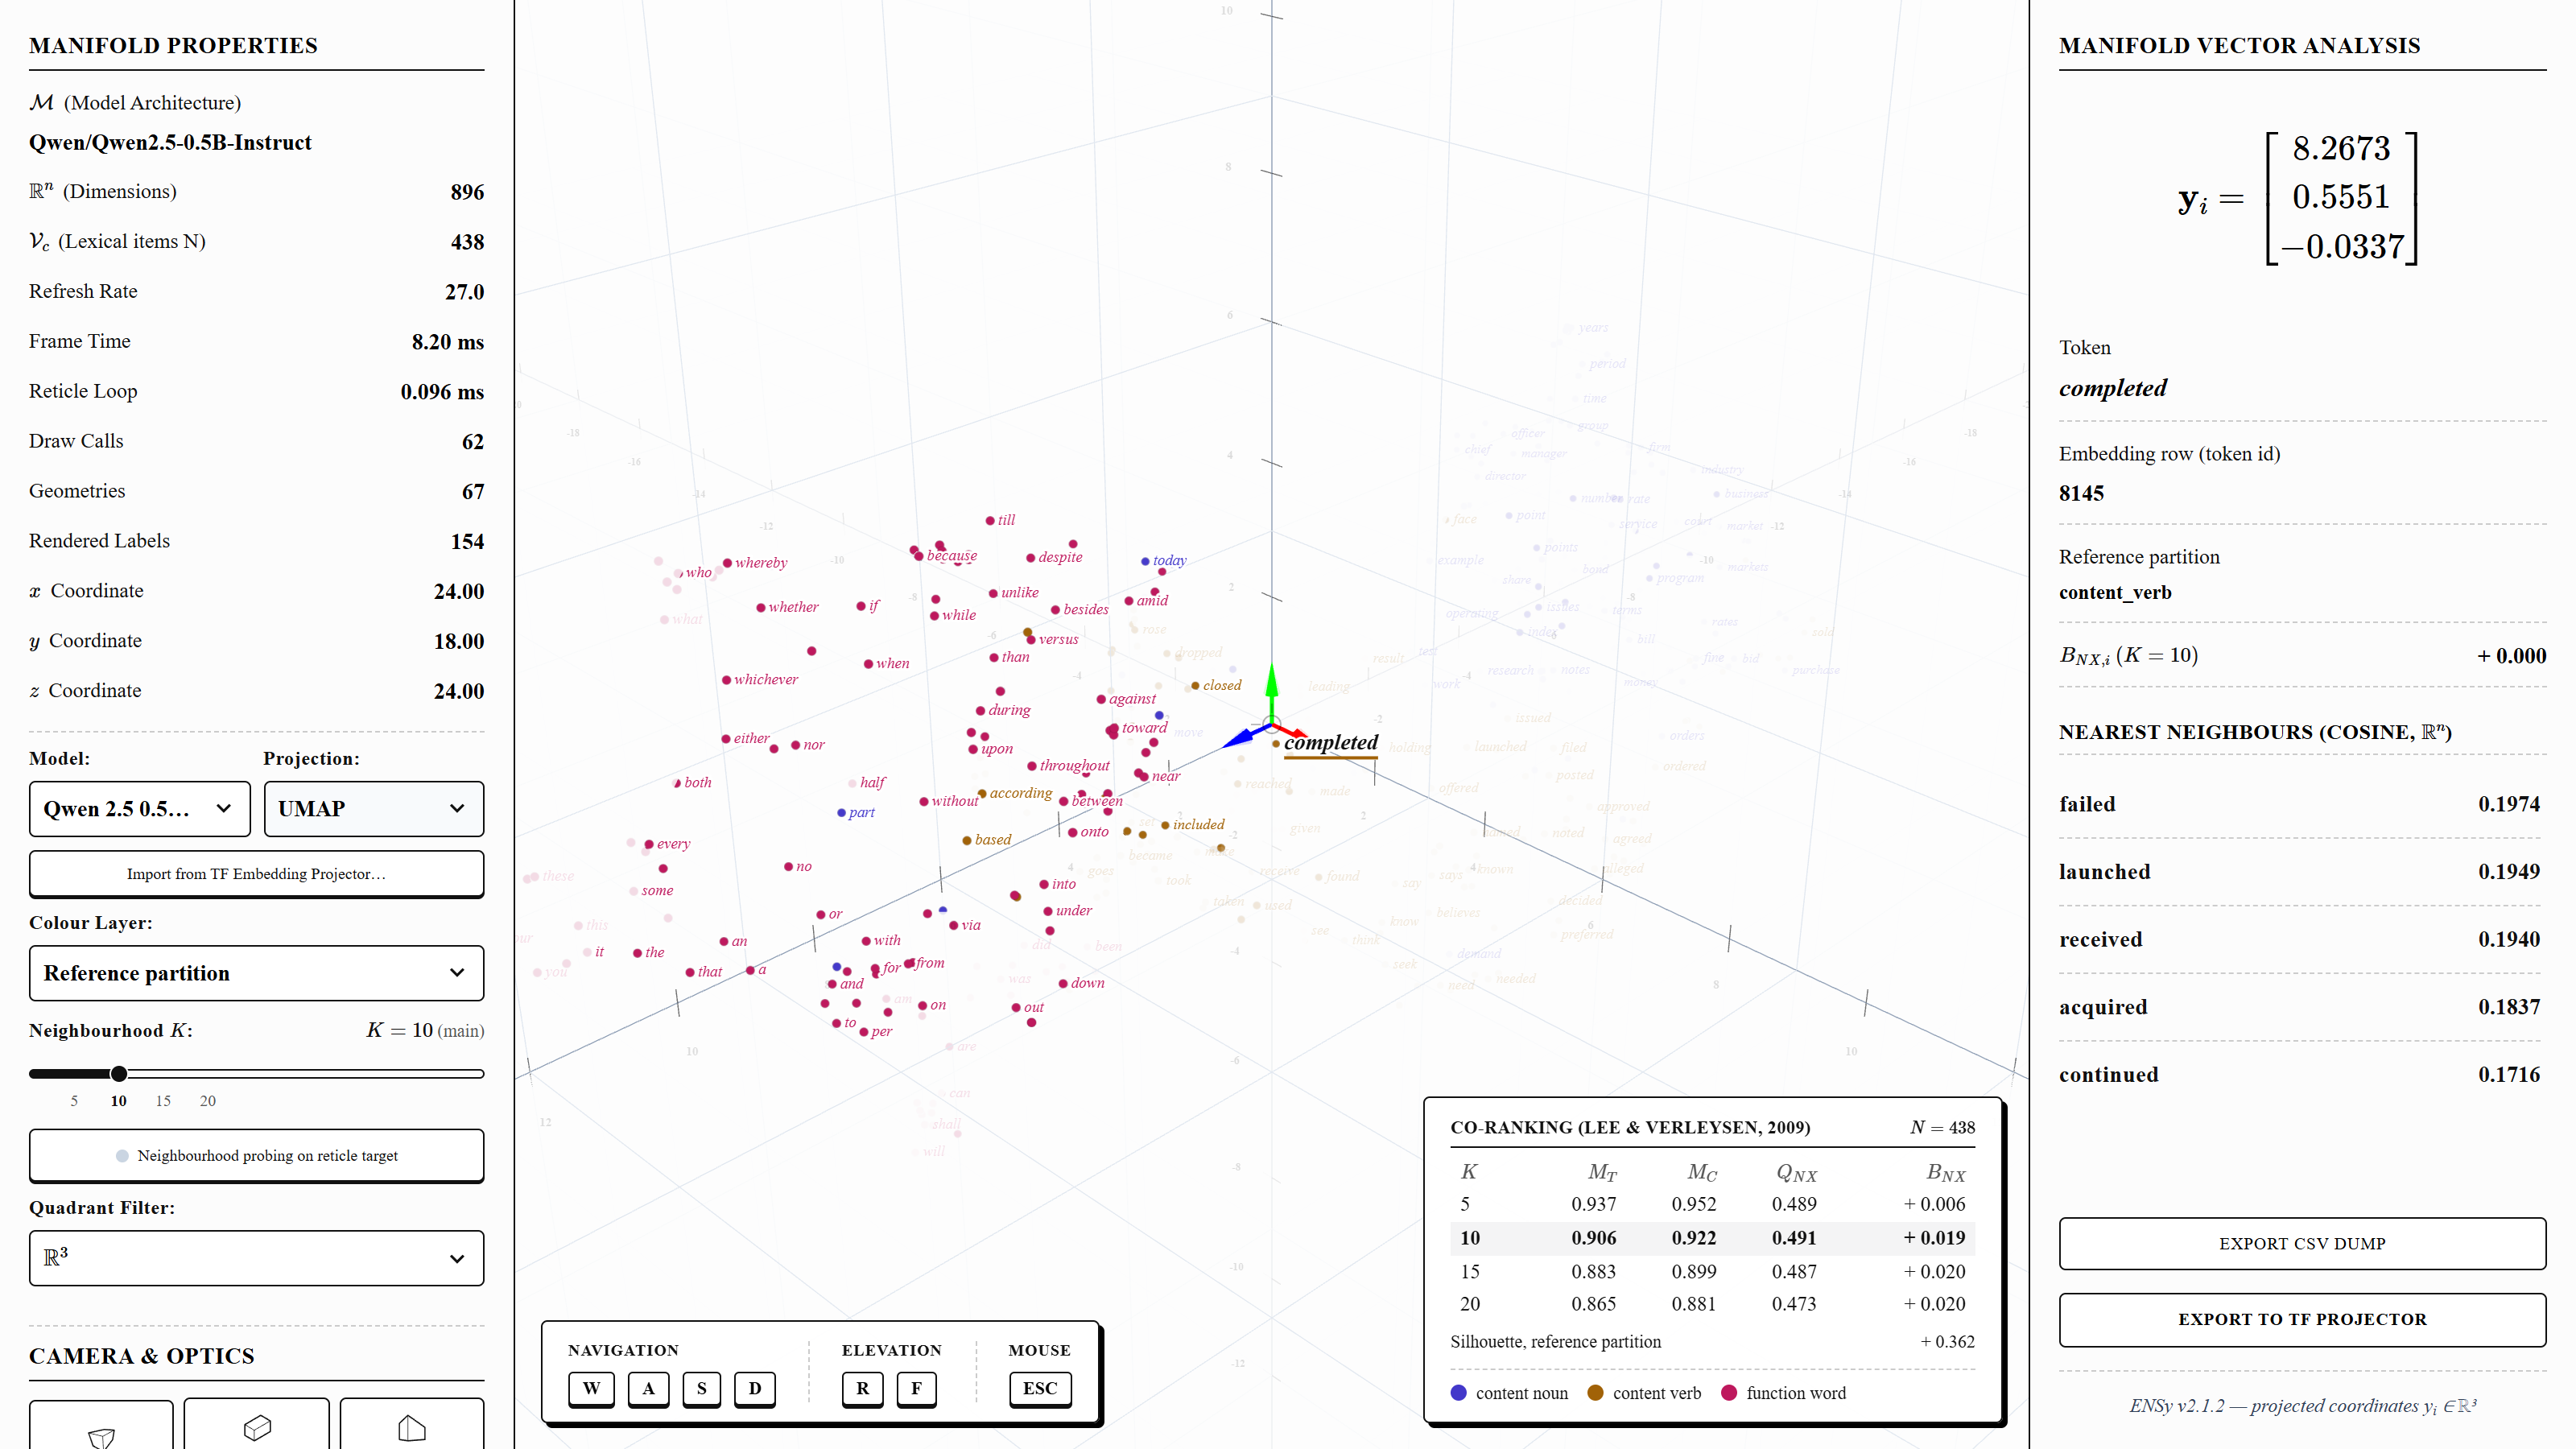
\includegraphics[width=\dimexpr\textwidth-2\fboxrule\relax,frame]{screenshots/fig01_workspace.png}
\caption{The ENSy workspace (Qwen 2.5, UMAP, isometric view). Left: model,
projection and colour layer selectors, the \(K\) slider, camera optics
and live profiling. Centre: the 438 tokens, coloured by the reference partition.
Bottom right: the co-ranking curves of the current projection. Right:
the inspector for the token under the reticle, with its true, false and
missing neighbours.}
\label{fig:workspace}
\end{figure*}

\subsection{Faithful rendering}\label{sec:faithful-rendering}

The rendered cloud is the projection itself: coordinates are placed with
a single isotropic similarity transform (median centre, one scale for
all axes, set by the 99th-percentile radius), which preserves all ratios
of distances. All tokens live in one \texttt{BufferGeometry} with
per-vertex RGBA colour (one draw call for the cloud regardless of
\(N\)). The dots write depth and are drawn before the semi-opaque grid
planes, so a plane dims the dots behind it but never hides those in
front. Every token is drawn as a dot, and a fog in the background colour
from the nearest to the farthest dot gives a depth cue, as in the
TensorFlow Embedding Projector. Words follow the same tool's strategy:
each frame they are drawn on one 2D canvas over the 3D view, to the
right of their dots, nearest tokens first, wherever they do not overlap
a word already placed, each with a white outline that separates it from
the dots behind it. A token whose word does not fit keeps only its dot,
and flying closer spreads the points so that more words fit.

\subsection{Colour layers and probing}\label{sec:colour-layers-probing}

Three layers share the colour channel with a fixed precedence ---
probing \textgreater{} behaviour map \textgreater{} reference partition
--- and never mix on one token. The \textbf{reference partition} colours
nouns, verbs and function words. The \textbf{behaviour map} rounds
\(B_{NX,i}(K)\) to the nearest multiple of 0.1, capped at \(\pm 0.3\),
and draws each of the seven steps in a colour-blind-safe diverging
palette (blue: extrusive; mid-grey: neutral; red: intrusive), with dots
up to 1.6 times larger as \(|B_{NX,i}|\) grows. The scale is fixed, never
normalised per frame, so equal values receive equal colours across
projections; it covers \(\pm 0.3\) rather than the theoretical range
\(\pm 1\) because the local values concentrate there: over the 20
configurations and \(K \in \{5, 10, 15, 20\}\), a median of 98\% of the
tokens (at least 86\%, at \(K = 5\)) have \(|B_{NX,i}(K)| \le 0.3\), and
a continuous ramp over \(\pm 1\) left almost every token pale. In this layer the colour is carried by the dot and the word
stays dark for legibility. \textbf{Probing} colours, for the token under the
reticle, its true (\(N_K \cap n_K\), green), false
(\(n_K \setminus N_K\), red) and missing (\(N_K \setminus n_K\),
translucent blue) neighbours.

\begin{figure*}[tp]
\centering
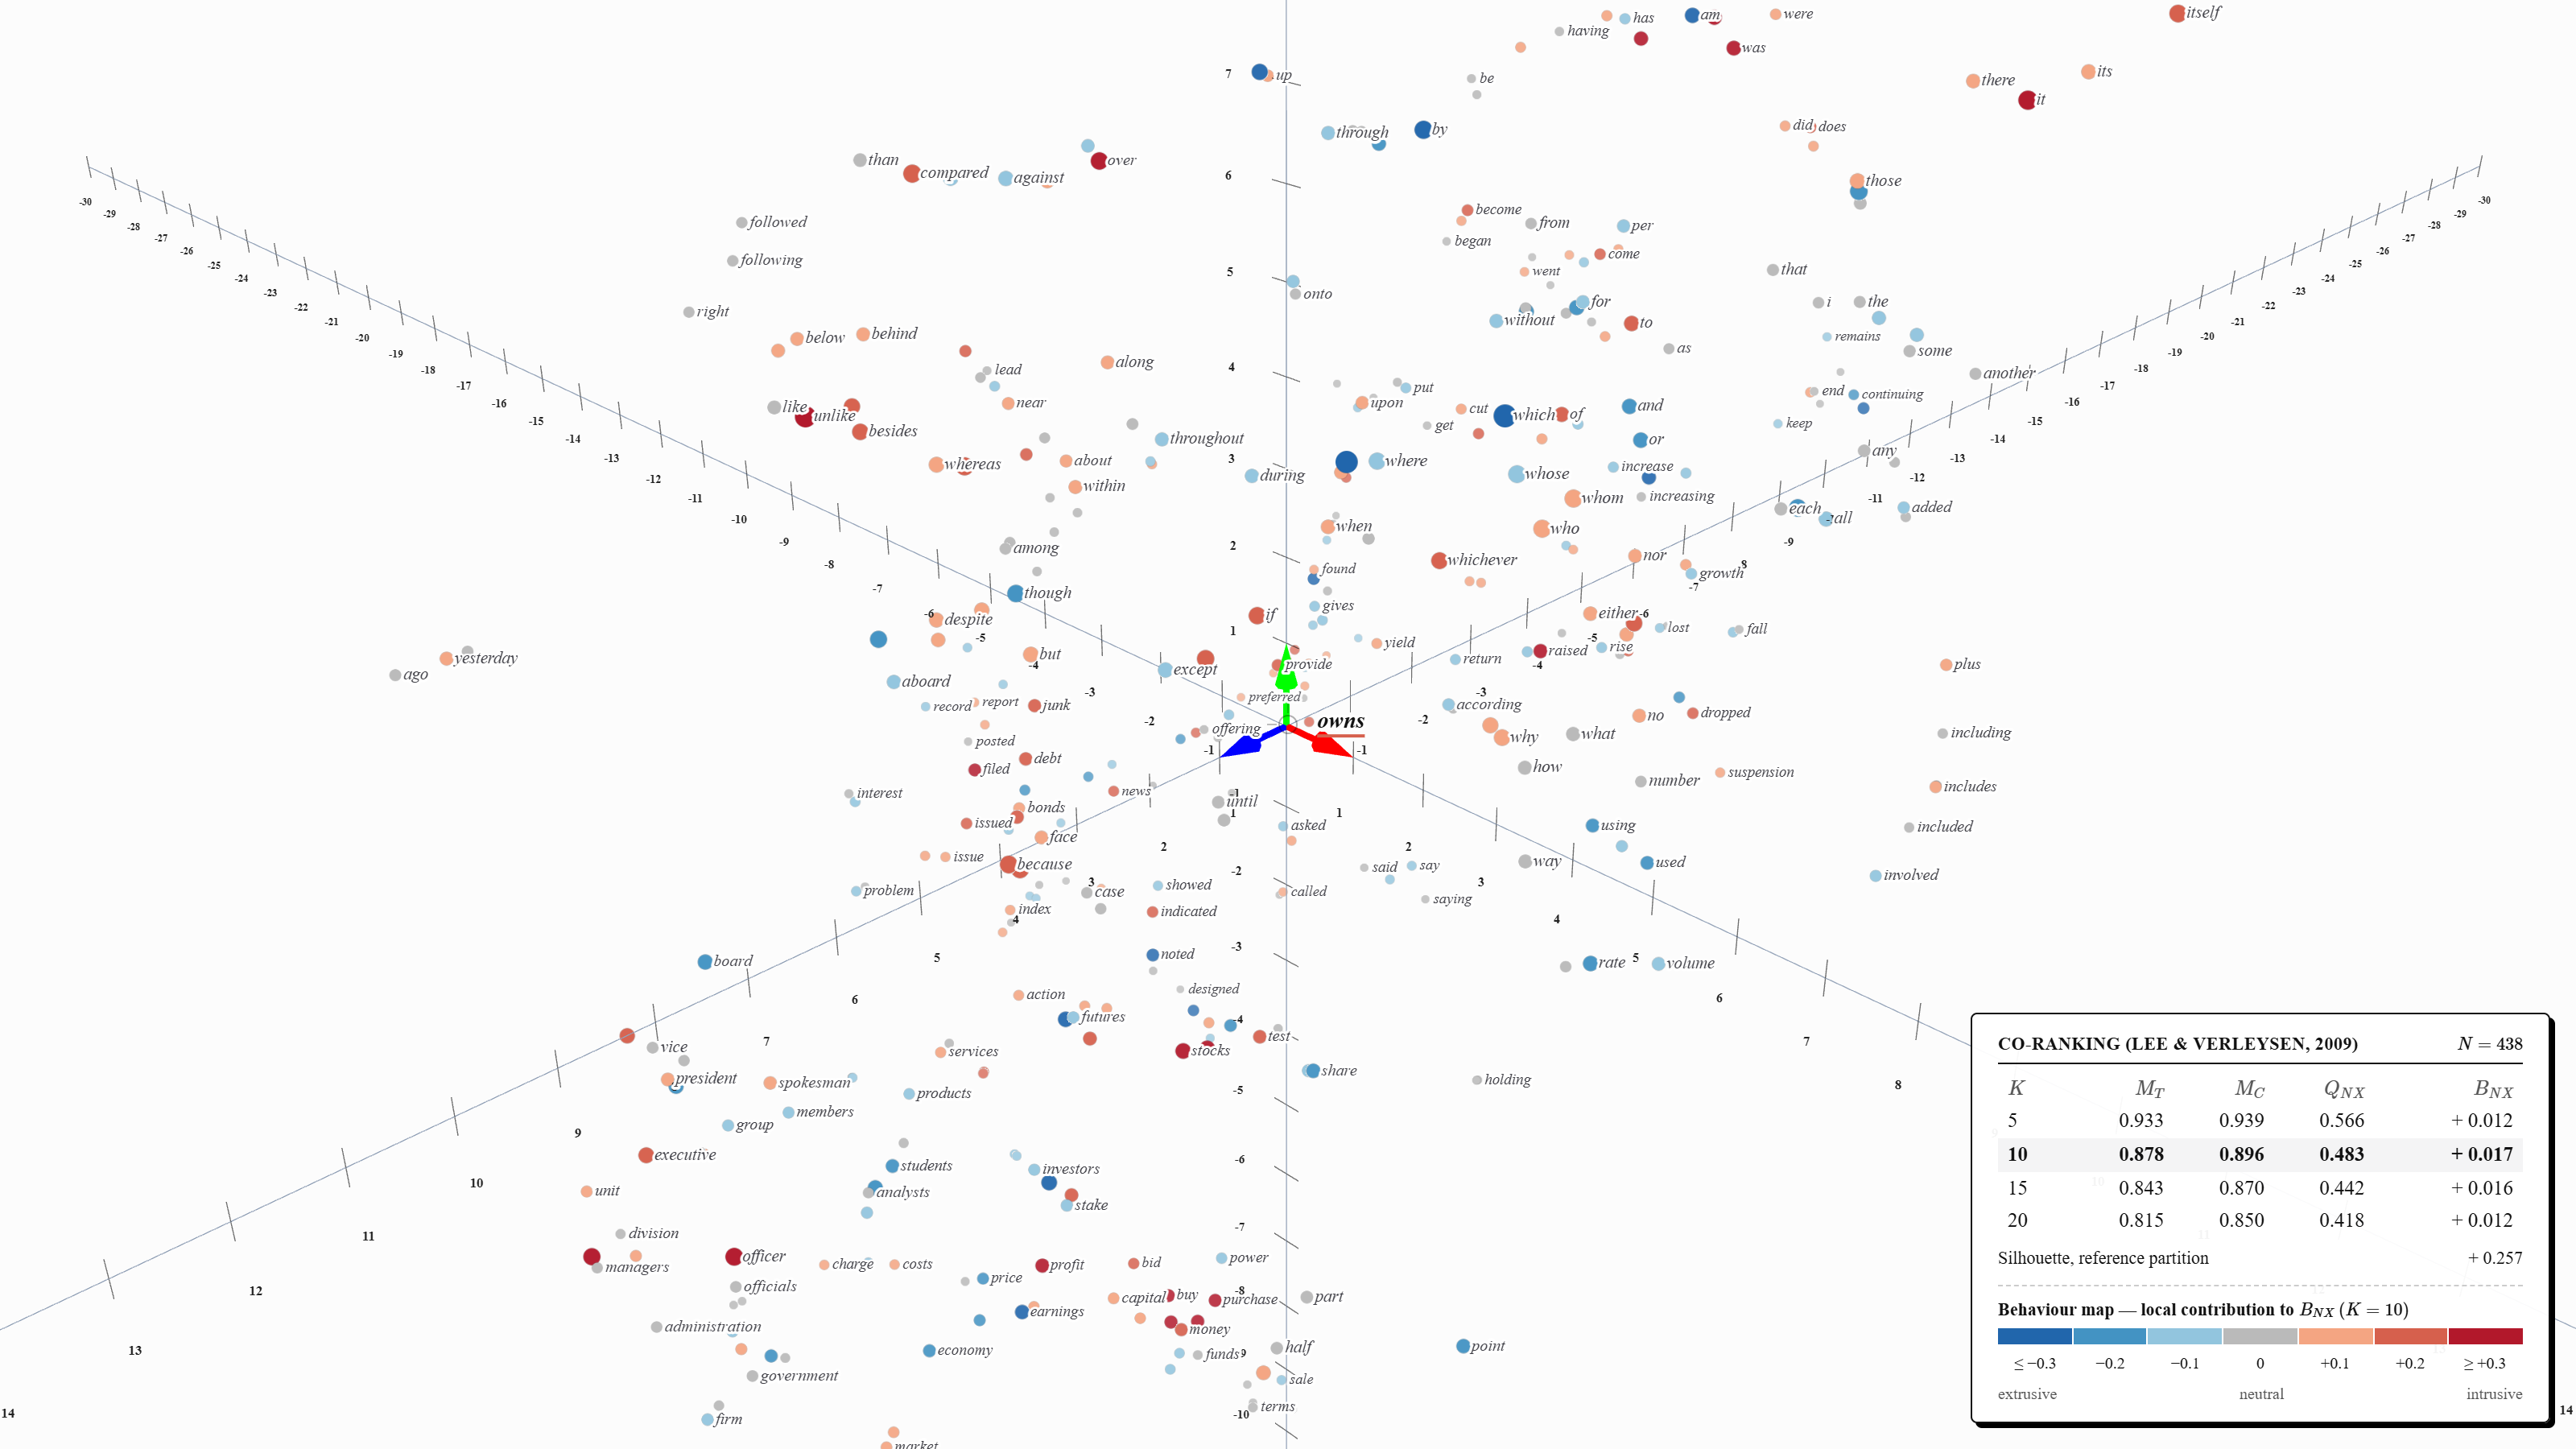
\includegraphics[width=\dimexpr\textwidth-2\fboxrule\relax,frame]{screenshots/fig04_behaviour_k10.png}
\caption{Behaviour map on Qwen 2.5 with t-SNE (perplexity 5), \(K = 10\)
(viewport only, grid planes off): each token's local contribution to
\(B_{NX}(10)\) on the fixed seven-step scale; larger dots mark larger
\(|B_{NX,i}|\).}
\label{fig:behaviour-k10}
\end{figure*}

\begin{figure*}[tp]
\centering
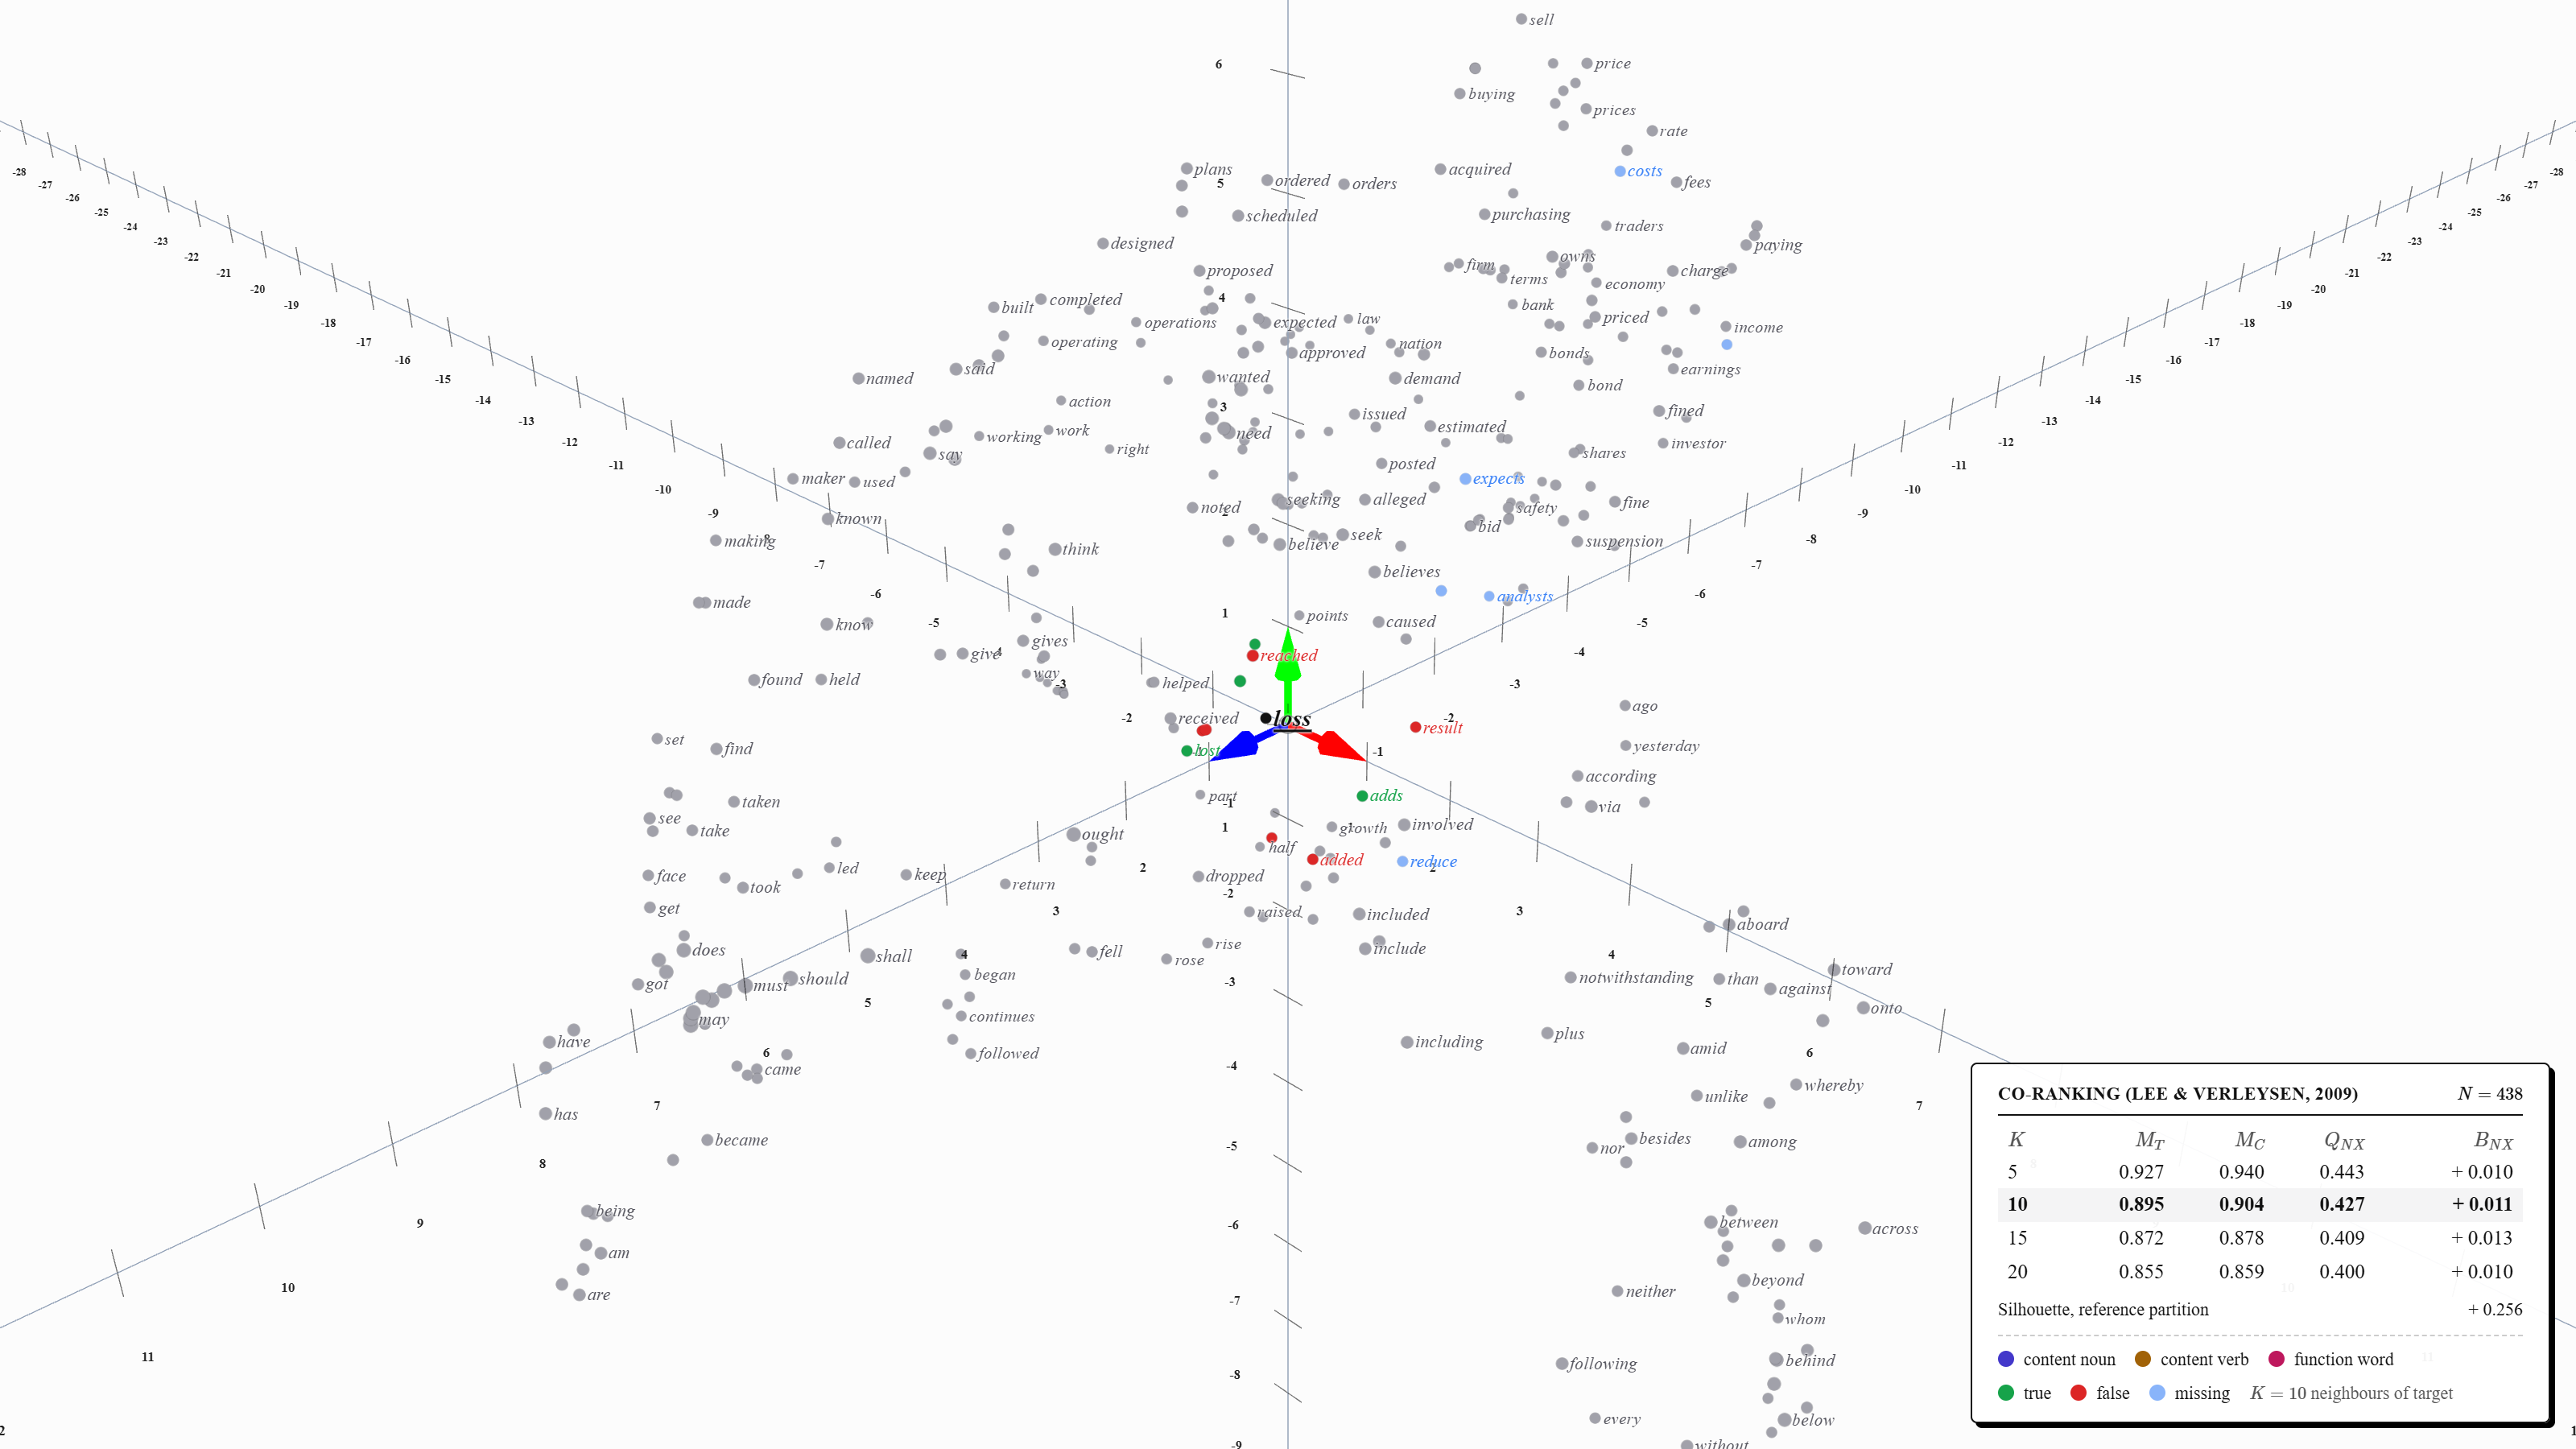
\includegraphics[width=\dimexpr\textwidth-2\fboxrule\relax,frame]{screenshots/fig06_probing.png}
\caption{Neighbourhood probing after flying towards a token (BERT, UMAP,
\(K = 10\); viewport only, grid planes off). Green: genuine neighbours
kept by the projection; red: false neighbours introduced by it;
translucent blue: genuine neighbours it pushed away; all other tokens
stay opaque in neutral grey.}
\label{fig:probing}
\end{figure*}

\subsection{Navigation and interface}\label{sec:navigation-interface}

The viewer offers first-person 6-DOF flight (W/A/S/D, R/F, mouse look
under pointer lock), perspective, parallel and two-point perspective
cameras with LERP/SLERP transitions between front, top, side and
isometric presets, an octant filter and a minimap. A central reticle
selects the nearest token in screen space within 25 px; the selected
word is drawn larger, in dark type, and underlined in the colour of its
dot, so it stays legible whatever its layer colour. The minimap is
omitted from the figures of this paper.

\begin{figure*}[tp]
\centering
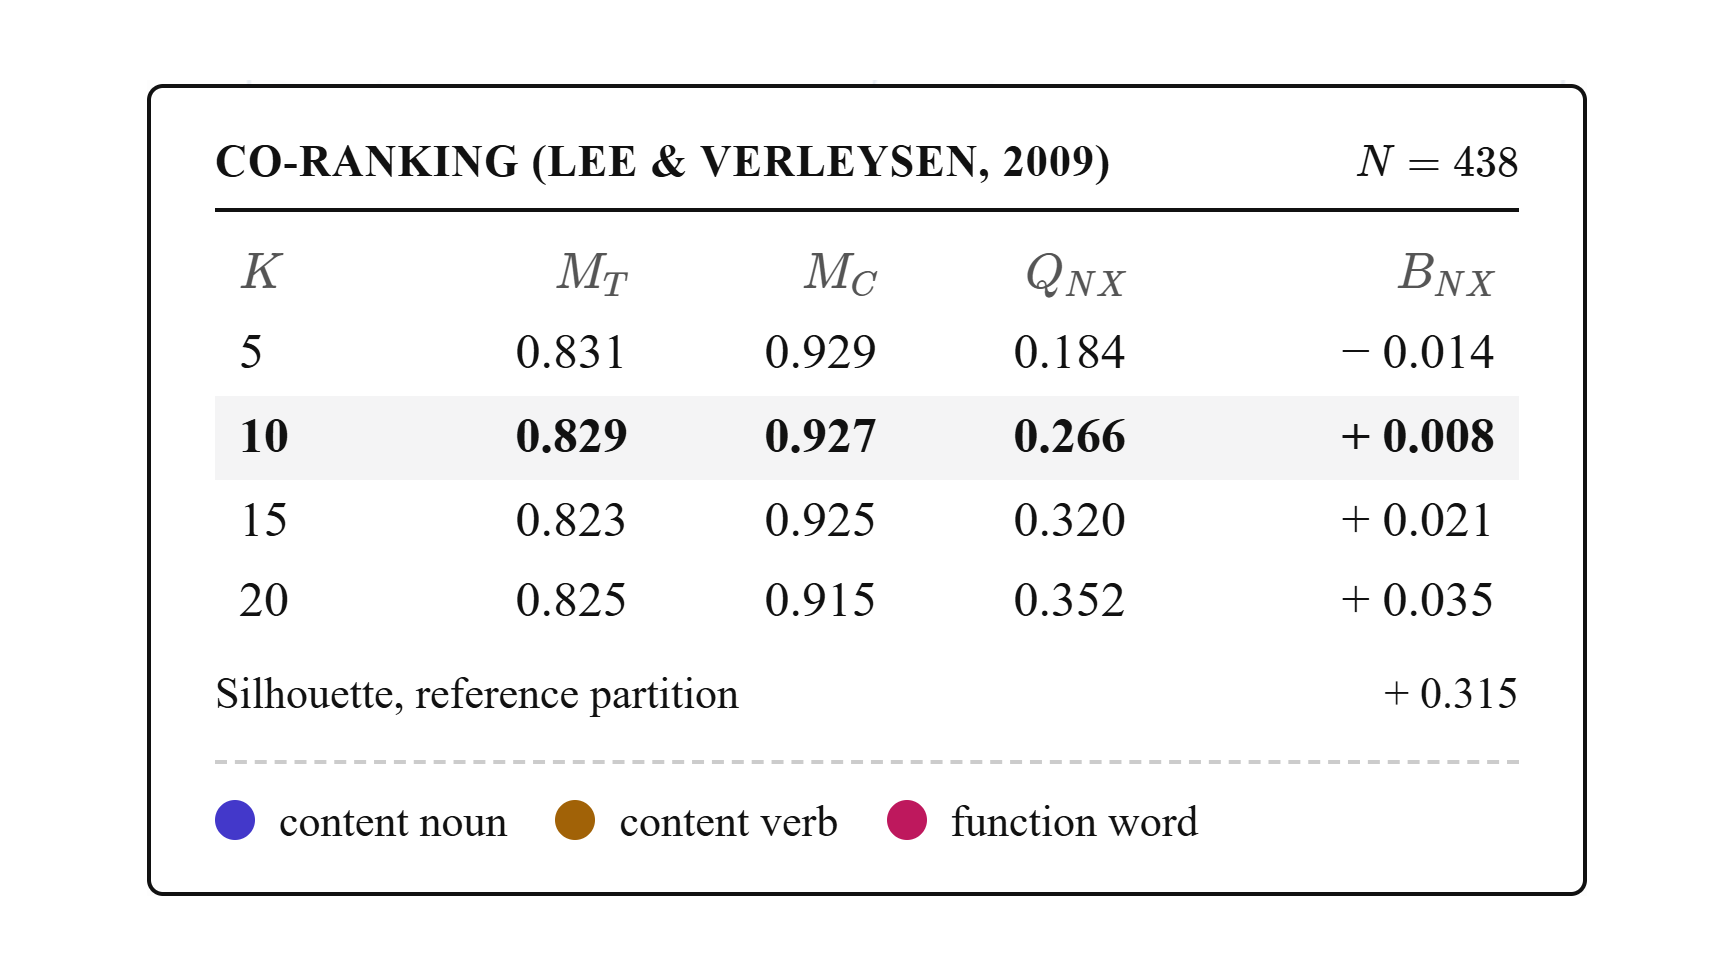
\includegraphics[width=\dimexpr\textwidth-2\fboxrule\relax,frame]{screenshots/fig08_metrics_panel.png}
\caption{Co-ranking panel for GPT-2 with Isomap: \(M_T\), \(M_C\), \(Q_{NX}\) and
\(B_{NX}\) over \(K\), and the Silhouette of the reference partition.}
\label{fig:metrics-panel}
\end{figure*}

\section{Results}\label{sec:results}

\subsection{Dataset}\label{sec:dataset}

The pipeline yields \(N = 438\) word types (146 per category); the
function words are the binding category. In the table, each multi-token
rejection is attributed to the first tokenizer that rejected it, in the
order Qwen, GPT-2, Gemma 2, BERT.

\subsection{Neighbourhood preservation}\label{sec:neighbourhood-preservation}

% BEGIN:main
\begin{table*}[tp]
\centering
\caption{Co-Ranking Metrics at $K = 10$ for Every Model and Projection}\label{tab:main}
\footnotesize
\begin{tabular*}{\textwidth}{@{\extracolsep{\fill}}llllllll@{}}
\toprule
Model & Algorithm & $M_T$ & $M_C$ & $Q_{NX}$ & $B_{NX}$ & $B_{TC}$ & $s$ \\
\midrule
Qwen 2.5 0.5B & PCA & 0.830 & 0.828 & 0.205 & $-0.007$ & $-0.001$ & $+0.161$ \\
Qwen 2.5 0.5B & t-SNE ($p=5$) & 0.875 & 0.891 & 0.477 & $+0.016$ & $+0.016$ & $+0.243$ \\
Qwen 2.5 0.5B & t-SNE ($p=30$) & 0.890 & 0.883 & 0.479 & $-0.041$ & $-0.008$ & $+0.153$ \\
Qwen 2.5 0.5B & UMAP & 0.899 & 0.923 & 0.486 & $+0.032$ & $+0.025$ & $+0.370$ \\
Qwen 2.5 0.5B & Isomap & 0.792 & 0.910 & 0.248 & $+0.028$ & $+0.117$ & $+0.281$ \\
GPT-2 & PCA & 0.827 & 0.846 & 0.216 & $-0.015$ & $+0.019$ & $+0.236$ \\
GPT-2 & t-SNE ($p=5$) & 0.896 & 0.914 & 0.457 & $+0.027$ & $+0.017$ & $+0.254$ \\
GPT-2 & t-SNE ($p=30$) & 0.912 & 0.912 & 0.495 & $-0.024$ & $+0.000$ & $+0.205$ \\
GPT-2 & UMAP & 0.917 & 0.938 & 0.474 & $+0.012$ & $+0.021$ & $+0.363$ \\
GPT-2 & Isomap & 0.829 & 0.927 & 0.266 & $+0.008$ & $+0.098$ & $+0.315$ \\
Gemma 2 2B & PCA & 0.867 & 0.802 & 0.189 & $-0.010$ & $-0.065$ & $+0.240$ \\
Gemma 2 2B & t-SNE ($p=5$) & 0.884 & 0.879 & 0.438 & $+0.013$ & $-0.005$ & $+0.234$ \\
Gemma 2 2B & t-SNE ($p=30$) & 0.901 & 0.909 & 0.432 & $-0.027$ & $+0.008$ & $+0.238$ \\
Gemma 2 2B & UMAP & 0.911 & 0.934 & 0.428 & $+0.005$ & $+0.022$ & $+0.345$ \\
Gemma 2 2B & Isomap & 0.864 & 0.920 & 0.238 & $+0.012$ & $+0.057$ & $+0.298$ \\
BERT base & PCA & 0.819 & 0.810 & 0.182 & $-0.005$ & $-0.008$ & $+0.159$ \\
BERT base & t-SNE ($p=5$) & 0.876 & 0.853 & 0.429 & $+0.001$ & $-0.023$ & $+0.201$ \\
BERT base & t-SNE ($p=30$) & 0.874 & 0.847 & 0.405 & $-0.039$ & $-0.027$ & $+0.181$ \\
BERT base & UMAP & 0.895 & 0.903 & 0.425 & $+0.014$ & $+0.008$ & $+0.261$ \\
BERT base & Isomap & 0.794 & 0.860 & 0.201 & $+0.012$ & $+0.066$ & $+0.166$ \\
\bottomrule
\end{tabular*}
\par\vspace{3pt}\parbox{\textwidth}{\scriptsize \emph{Source: \texttt{results/main\_c2416895b599.json} --- commit \texttt{e7f5a91f} (clean working tree), Python 3.12.14, scikit-learn 1.6.1, umap-learn 0.5.7, seed 42, extraction: HTTP Range rows.}}
\end{table*}
% END:main

\(s\): Silhouette of the reference partition in the 3D projection. For
reference, the Silhouette in the original space and the variance
captured by three principal components:

% BEGIN:highdim
\begin{table*}[tp]
\centering
\caption{Original-Space Silhouette and PCA Variance}\label{tab:highdim}
\footnotesize
\begin{tabular*}{\textwidth}{@{\extracolsep{\fill}}llll@{}}
\toprule
Model & $d$ & $s$ in $\mathbb{R}^d$ (cosine) & PCA variance, 3 components \\
\midrule
Qwen 2.5 0.5B & 896 & $+0.031$ & 7.8\% \\
GPT-2 & 768 & $+0.048$ & 10.7\% \\
Gemma 2 2B & 2304 & $+0.044$ & 10.9\% \\
BERT base & 768 & $+0.025$ & 11.0\% \\
\bottomrule
\end{tabular*}
\end{table*}
% END:highdim

% BEGIN:curves_mt
\begin{figure*}[tp]
\centering
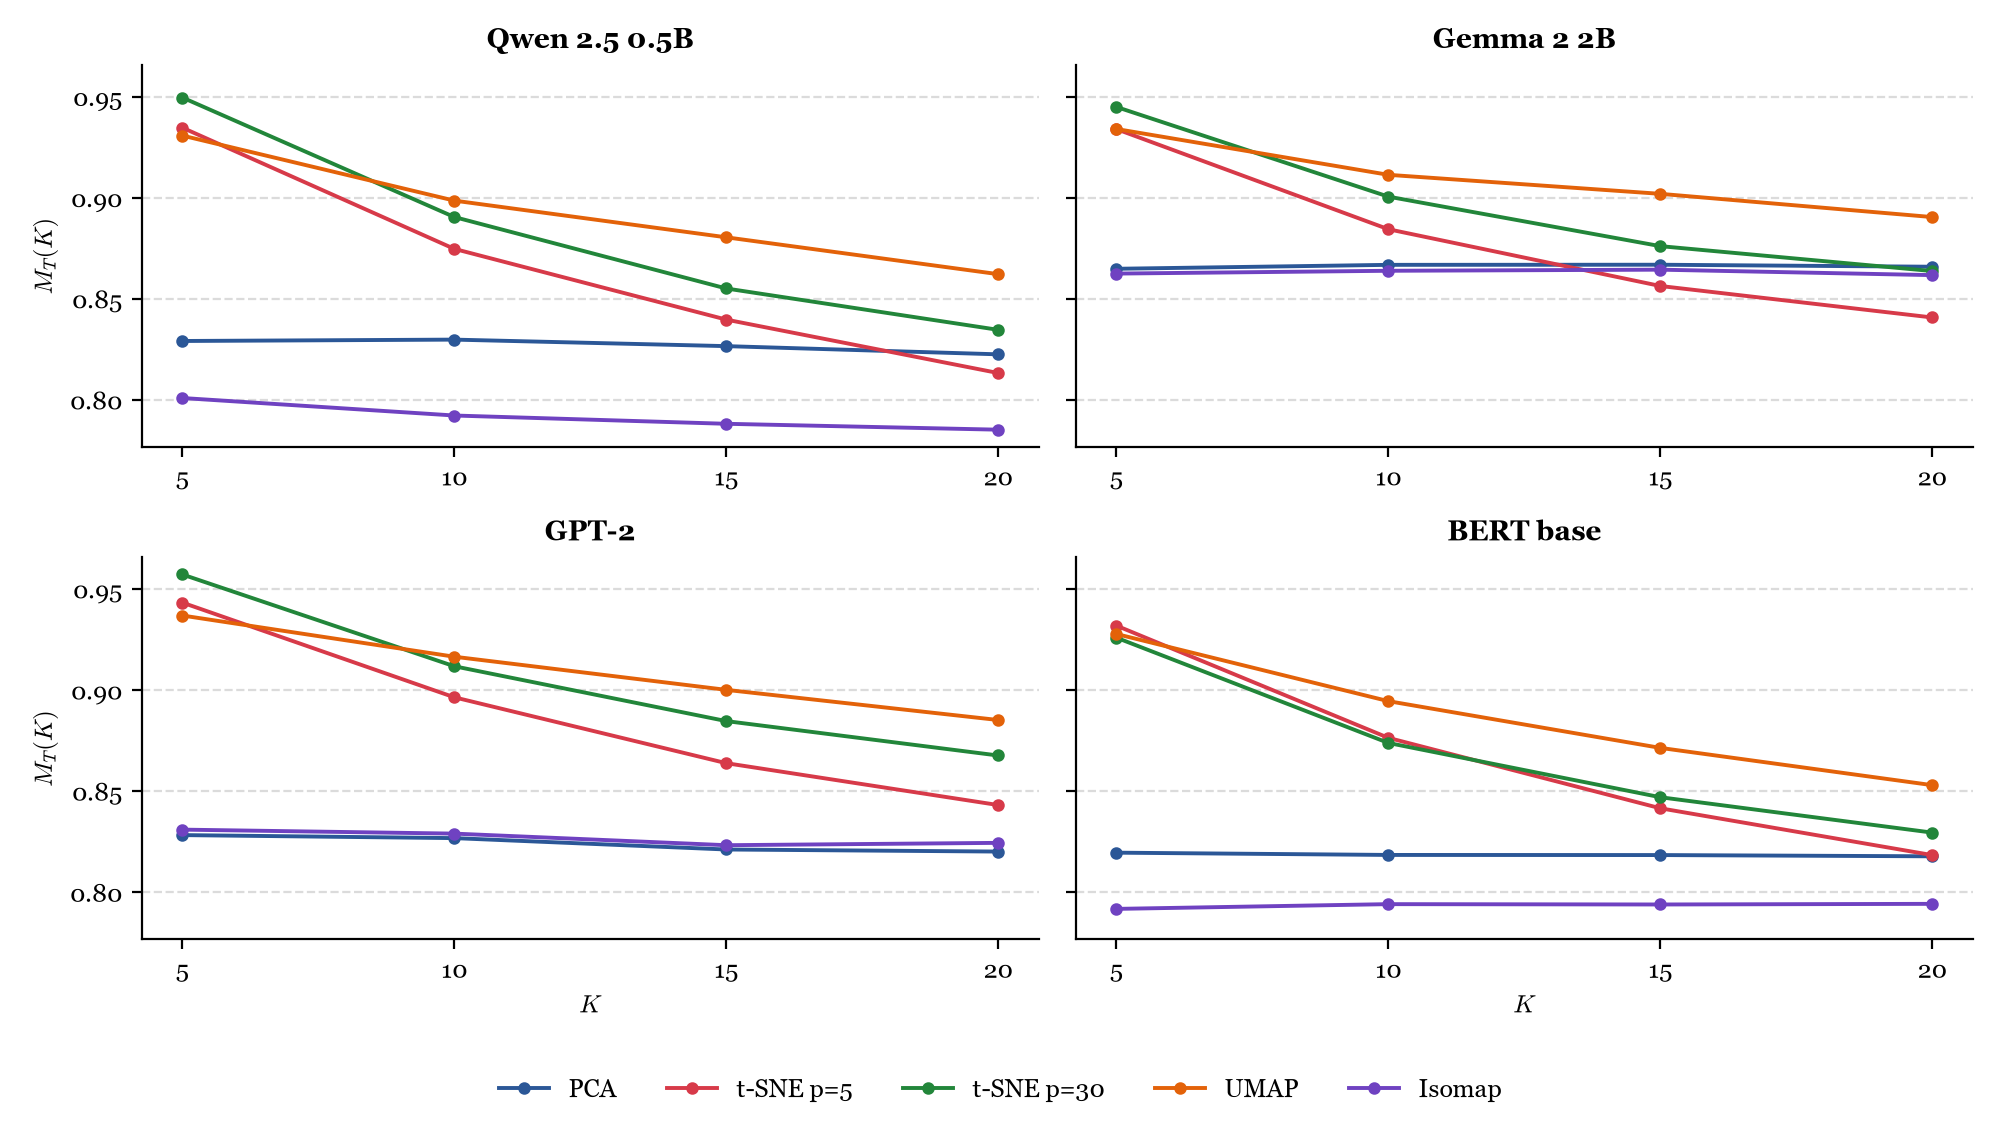
\includegraphics[width=\dimexpr\textwidth-2\fboxrule\relax,frame]{figures/curves_trustworthiness.png}
\caption{Trustworthiness $M_T(K)$ over $K$ for every model and projection configuration.}\label{fig:curves-trustworthiness}
\end{figure*}
% END:curves_mt

% BEGIN:curves_bnx
\begin{figure*}[tp]
\centering
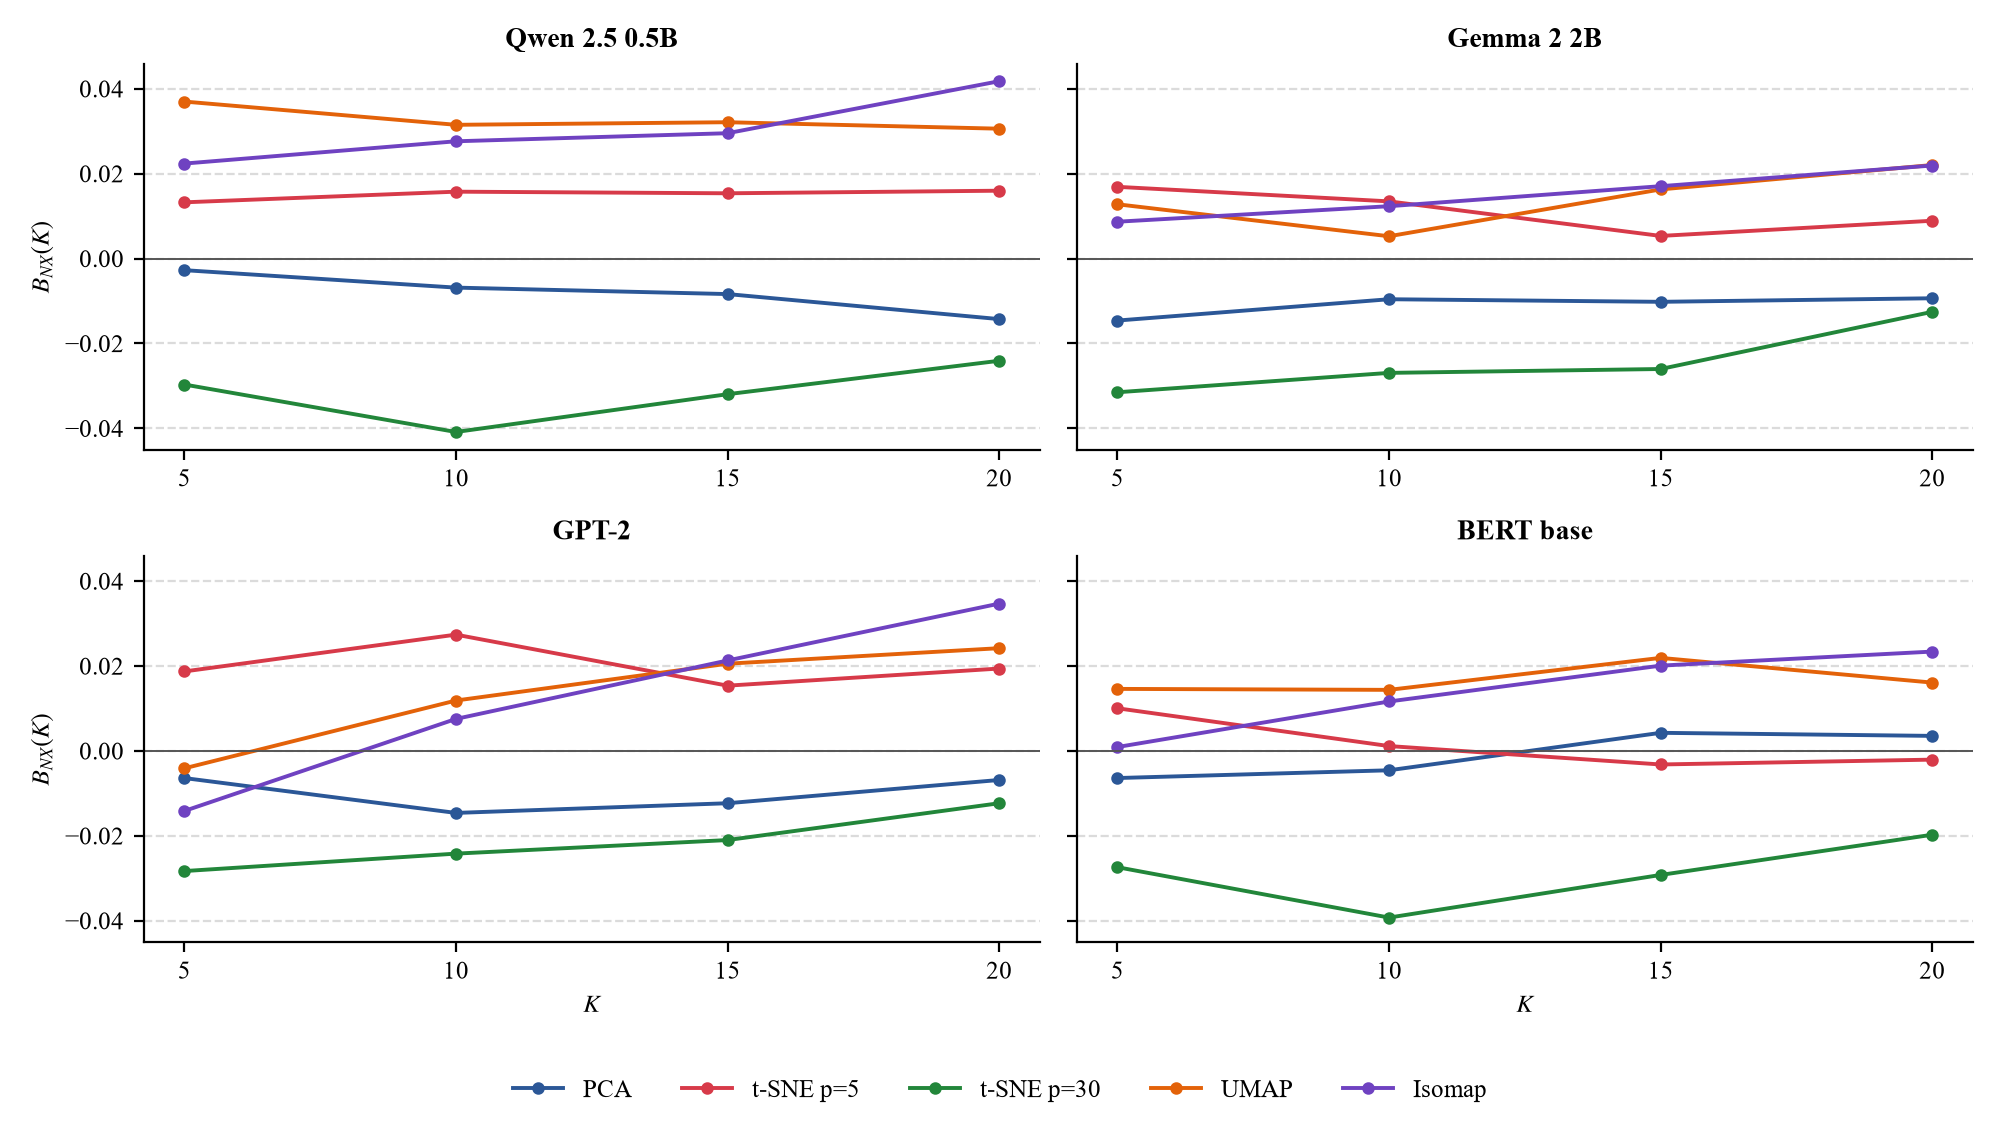
\includegraphics[width=\dimexpr\textwidth-2\fboxrule\relax,frame]{figures/curves_bnx.png}
\caption{Behaviour indicator $B_{NX}(K)$ over $K$ (positive: intrusive; negative: extrusive). With perplexity 30, t-SNE is below zero at every $K$ in all four models; with perplexity 5 it is above zero for Qwen, Gemma 2 and GPT-2 and close to zero for BERT.}\label{fig:curves-bnx}
\end{figure*}
% END:curves_bnx

\subsection{Visual comparison}\label{sec:visual-comparison}

Figs.~\ref{fig:pca}--\ref{fig:isomap} show the five projection configurations of the same model,
and Figs.~\ref{fig:qwen}--\ref{fig:bert} the same algorithm (UMAP) across the four models. All
are seen from the same camera (isometric preset, then a one-second
forward flight along the aim), with the grid planes switched off.
Colours: indigo nouns, ochre verbs, magenta function words.

\begin{figure*}[tp]
\centering
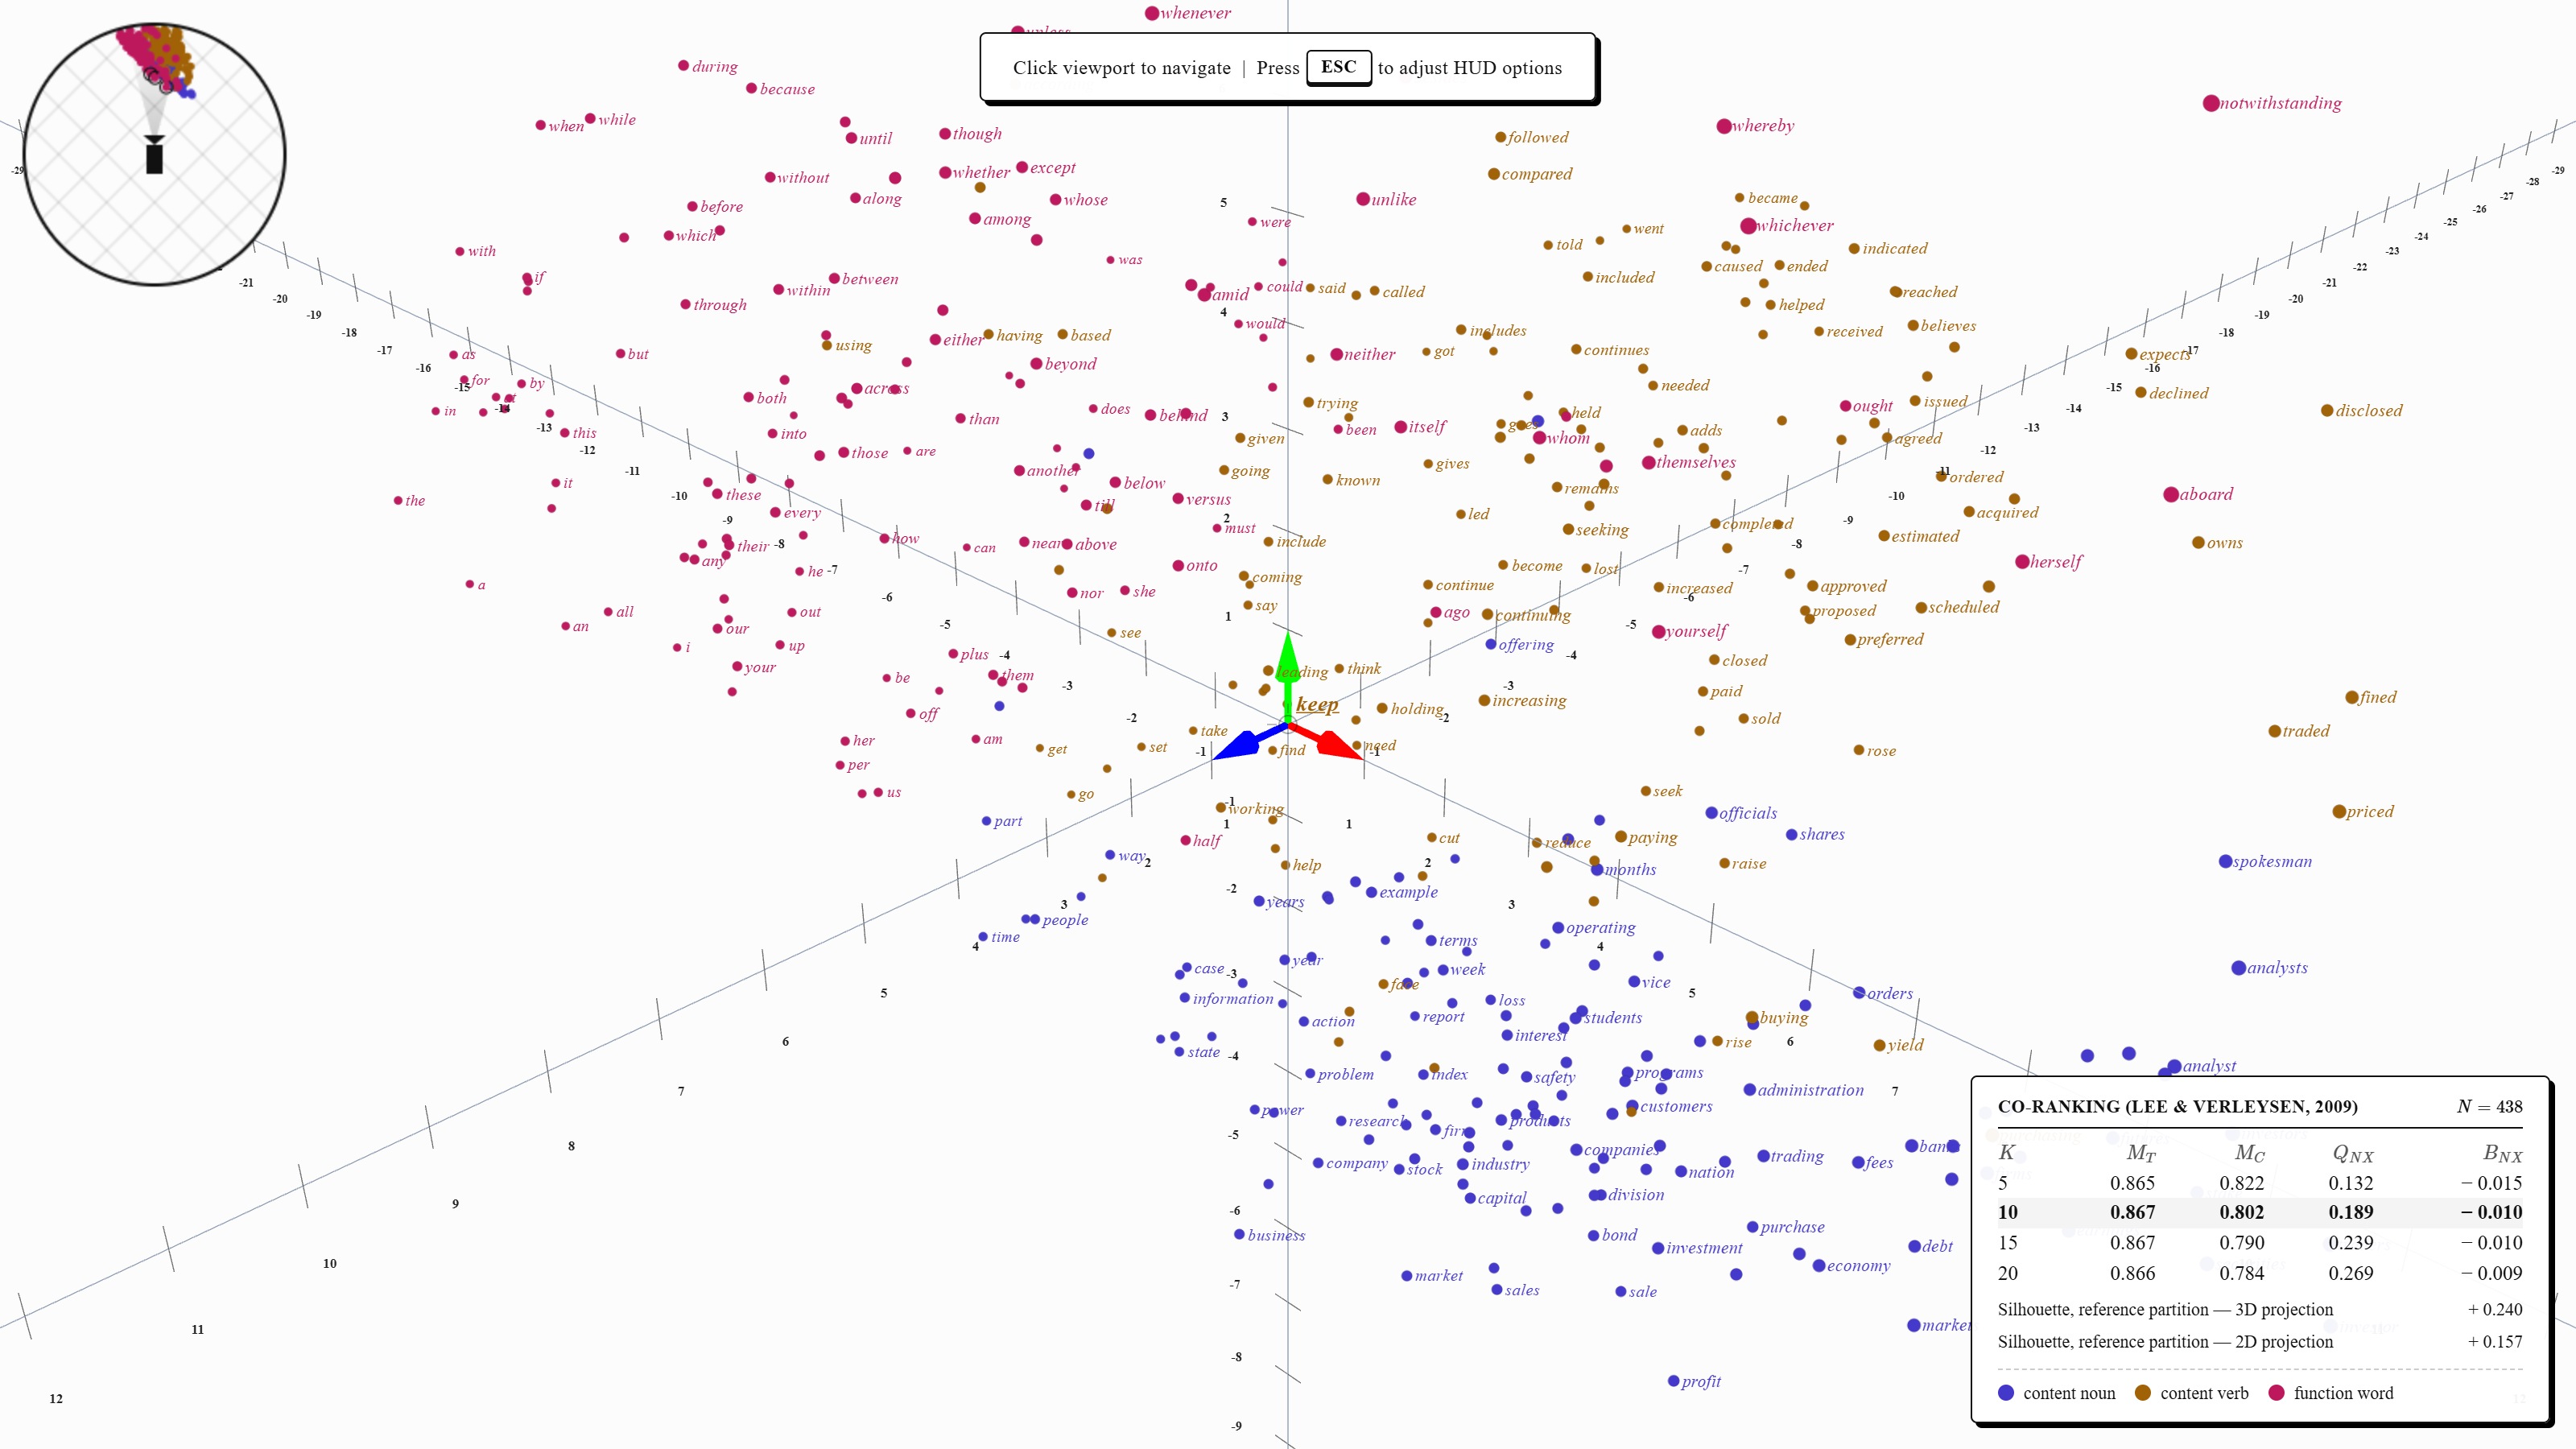
\includegraphics[width=\dimexpr\textwidth-2\fboxrule\relax,frame]{screenshots/fig02_pca.png}
\caption{Gemma 2 2B --- PCA (centred).}
\label{fig:pca}
\end{figure*}

\begin{figure*}[tp]
\centering
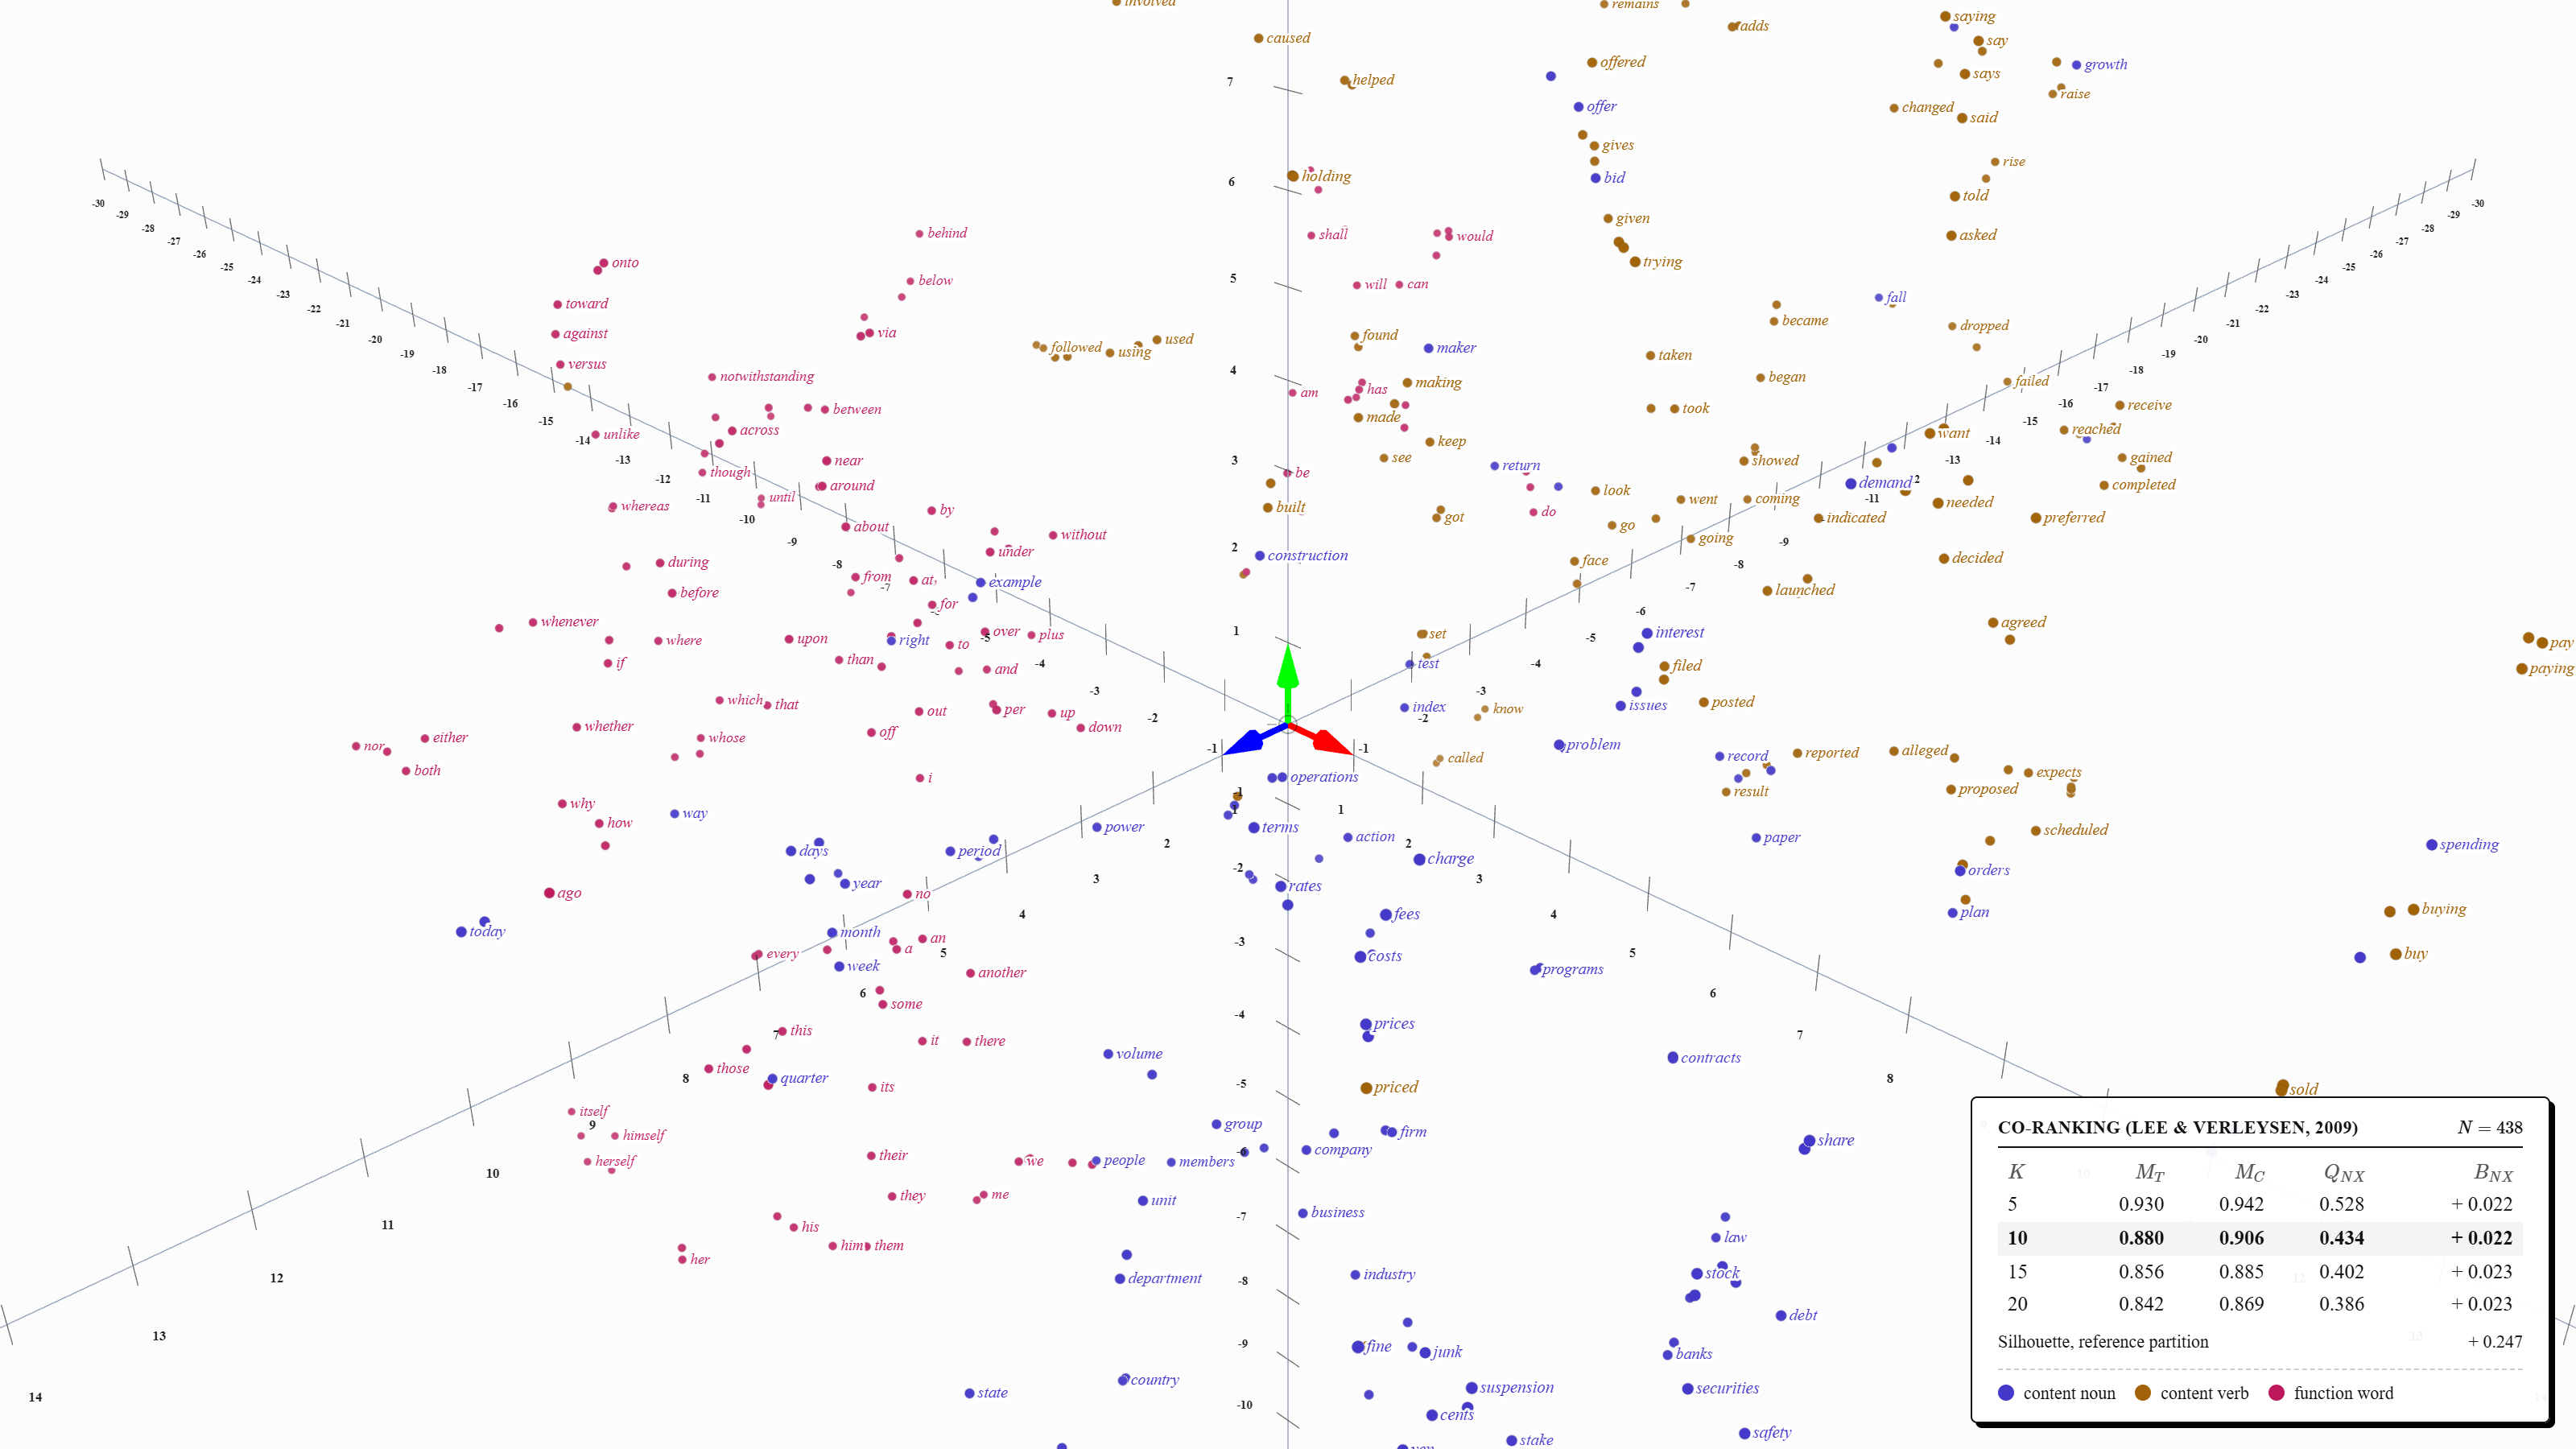
\includegraphics[width=\dimexpr\textwidth-2\fboxrule\relax,frame]{screenshots/fig02_tsne.png}
\caption{Gemma 2 2B --- t-SNE, perplexity 5.}
\label{fig:tsne}
\end{figure*}

\begin{figure*}[tp]
\centering
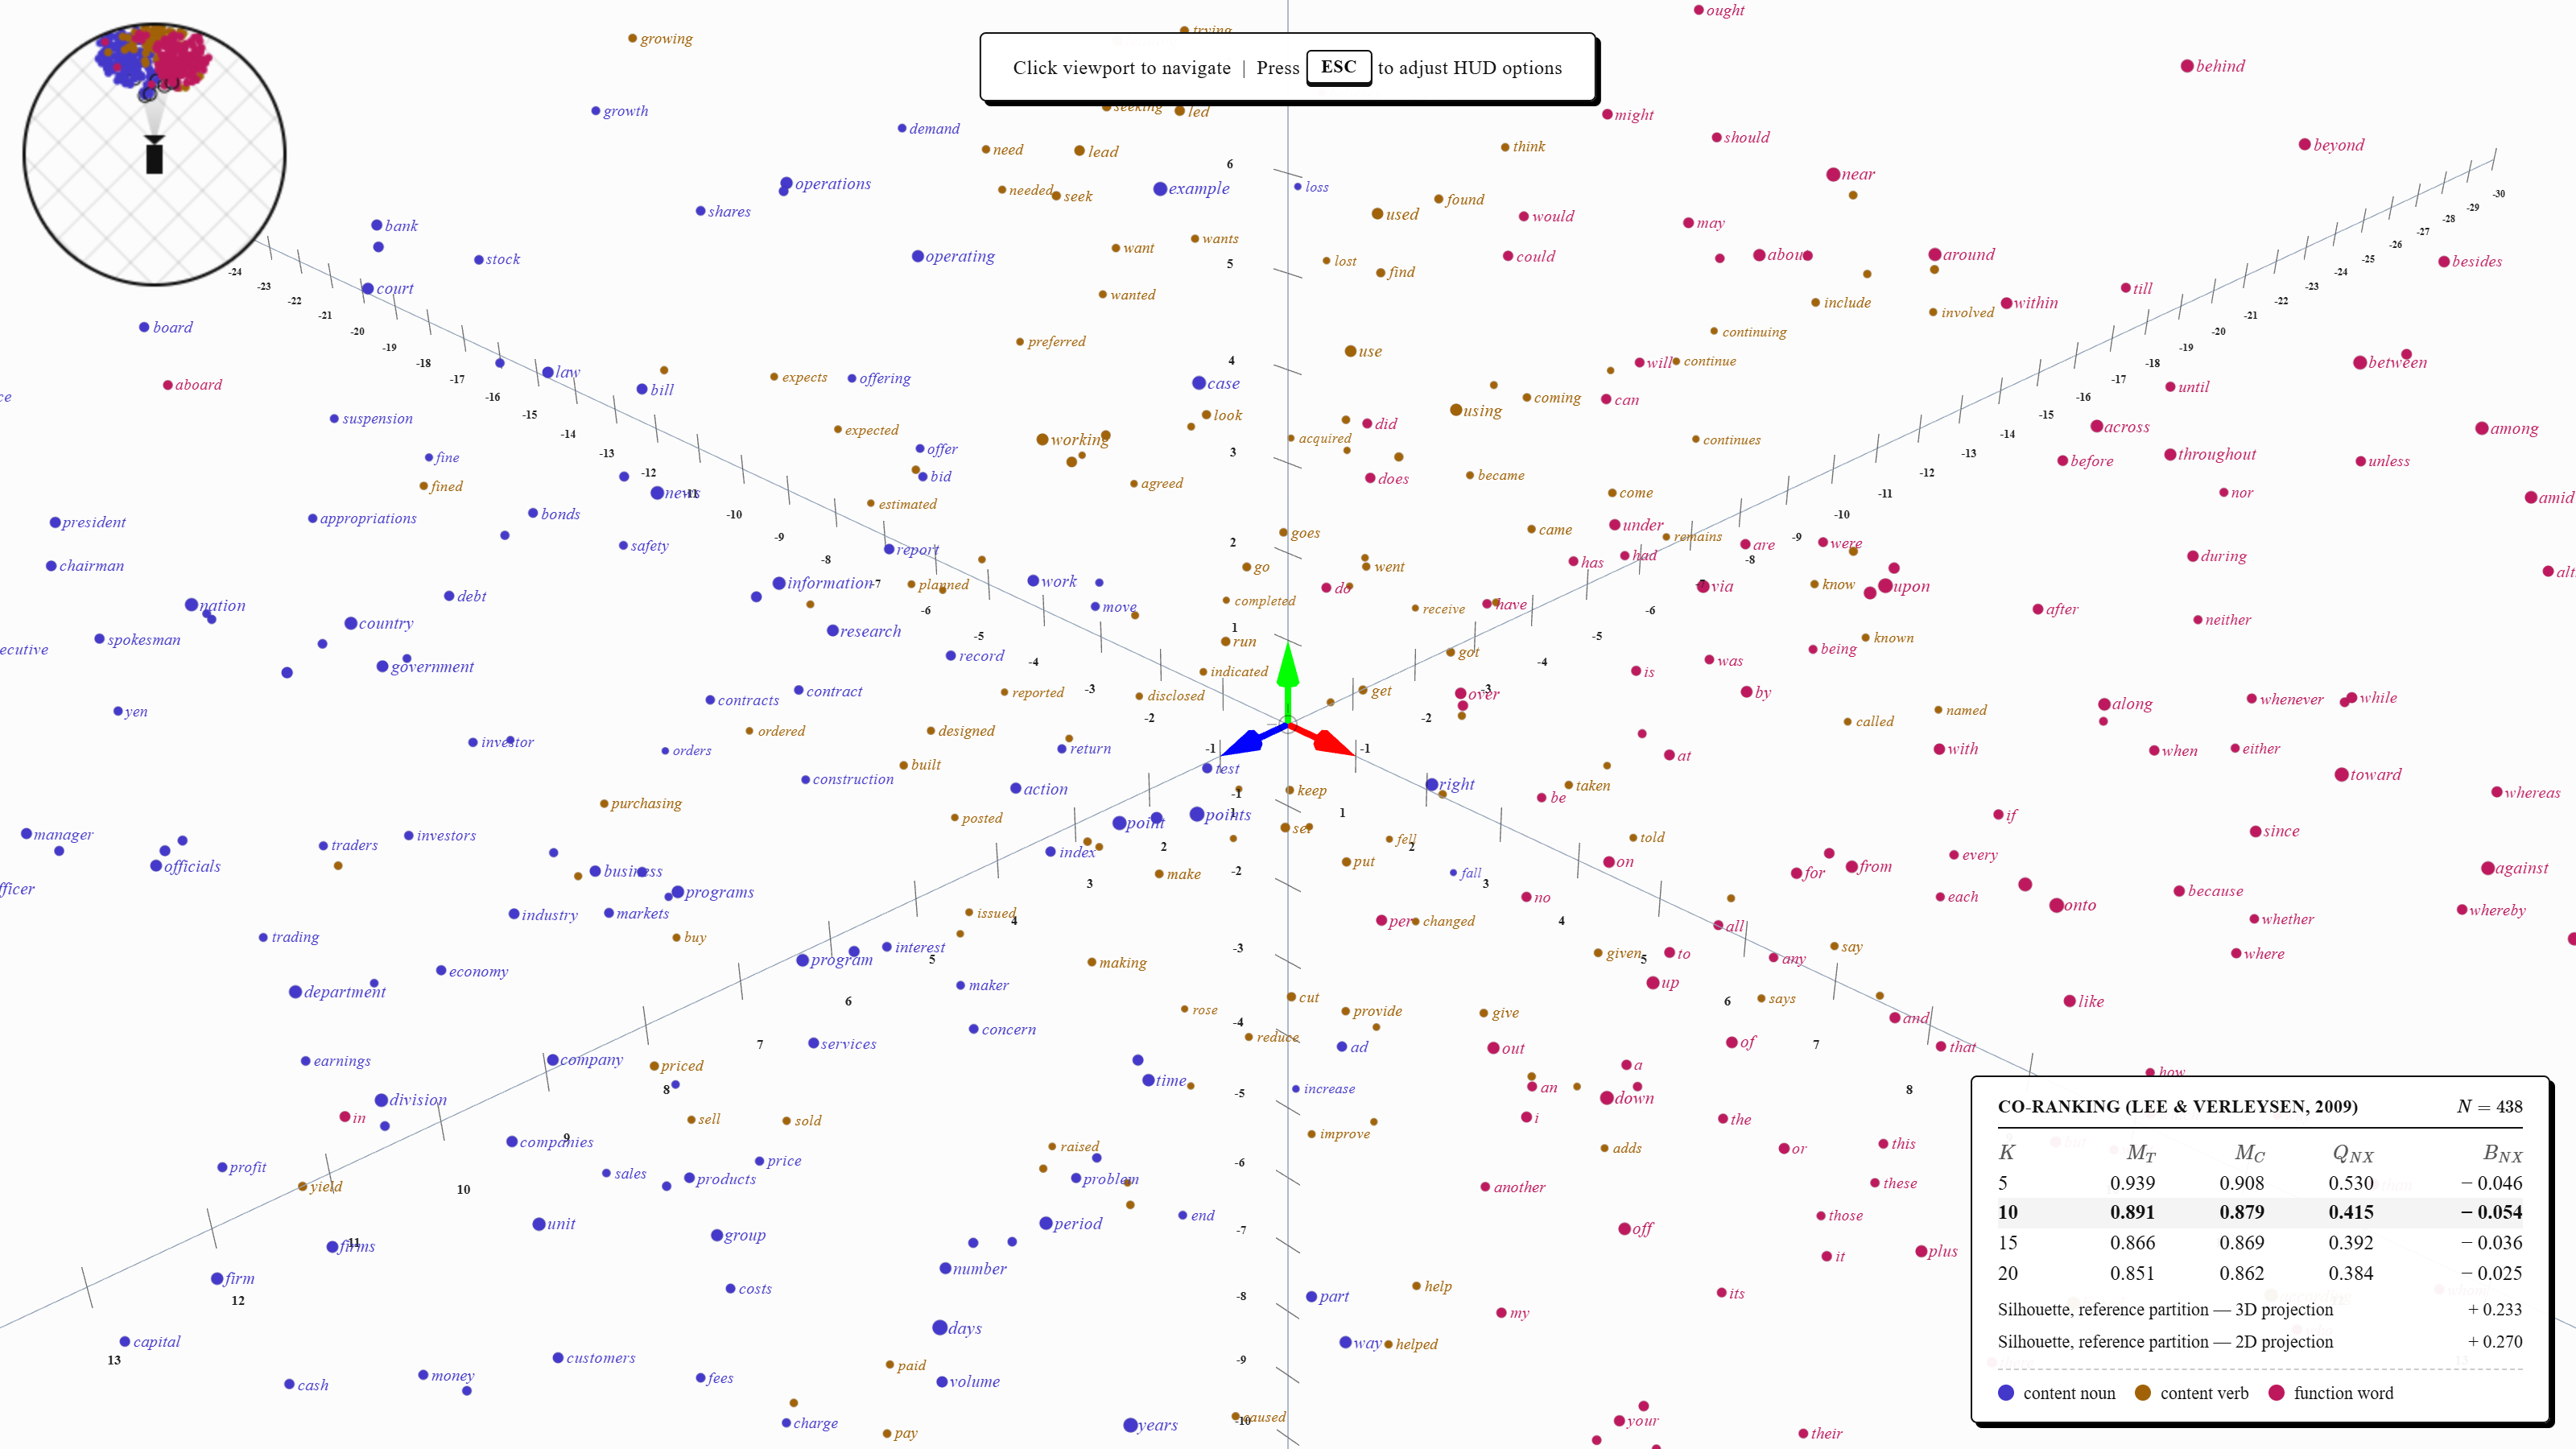
\includegraphics[width=\dimexpr\textwidth-2\fboxrule\relax,frame]{screenshots/fig02_tsne_p30.png}
\caption{Gemma 2 2B --- t-SNE, perplexity 30.}
\label{fig:tsne-p30}
\end{figure*}

\begin{figure*}[tp]
\centering
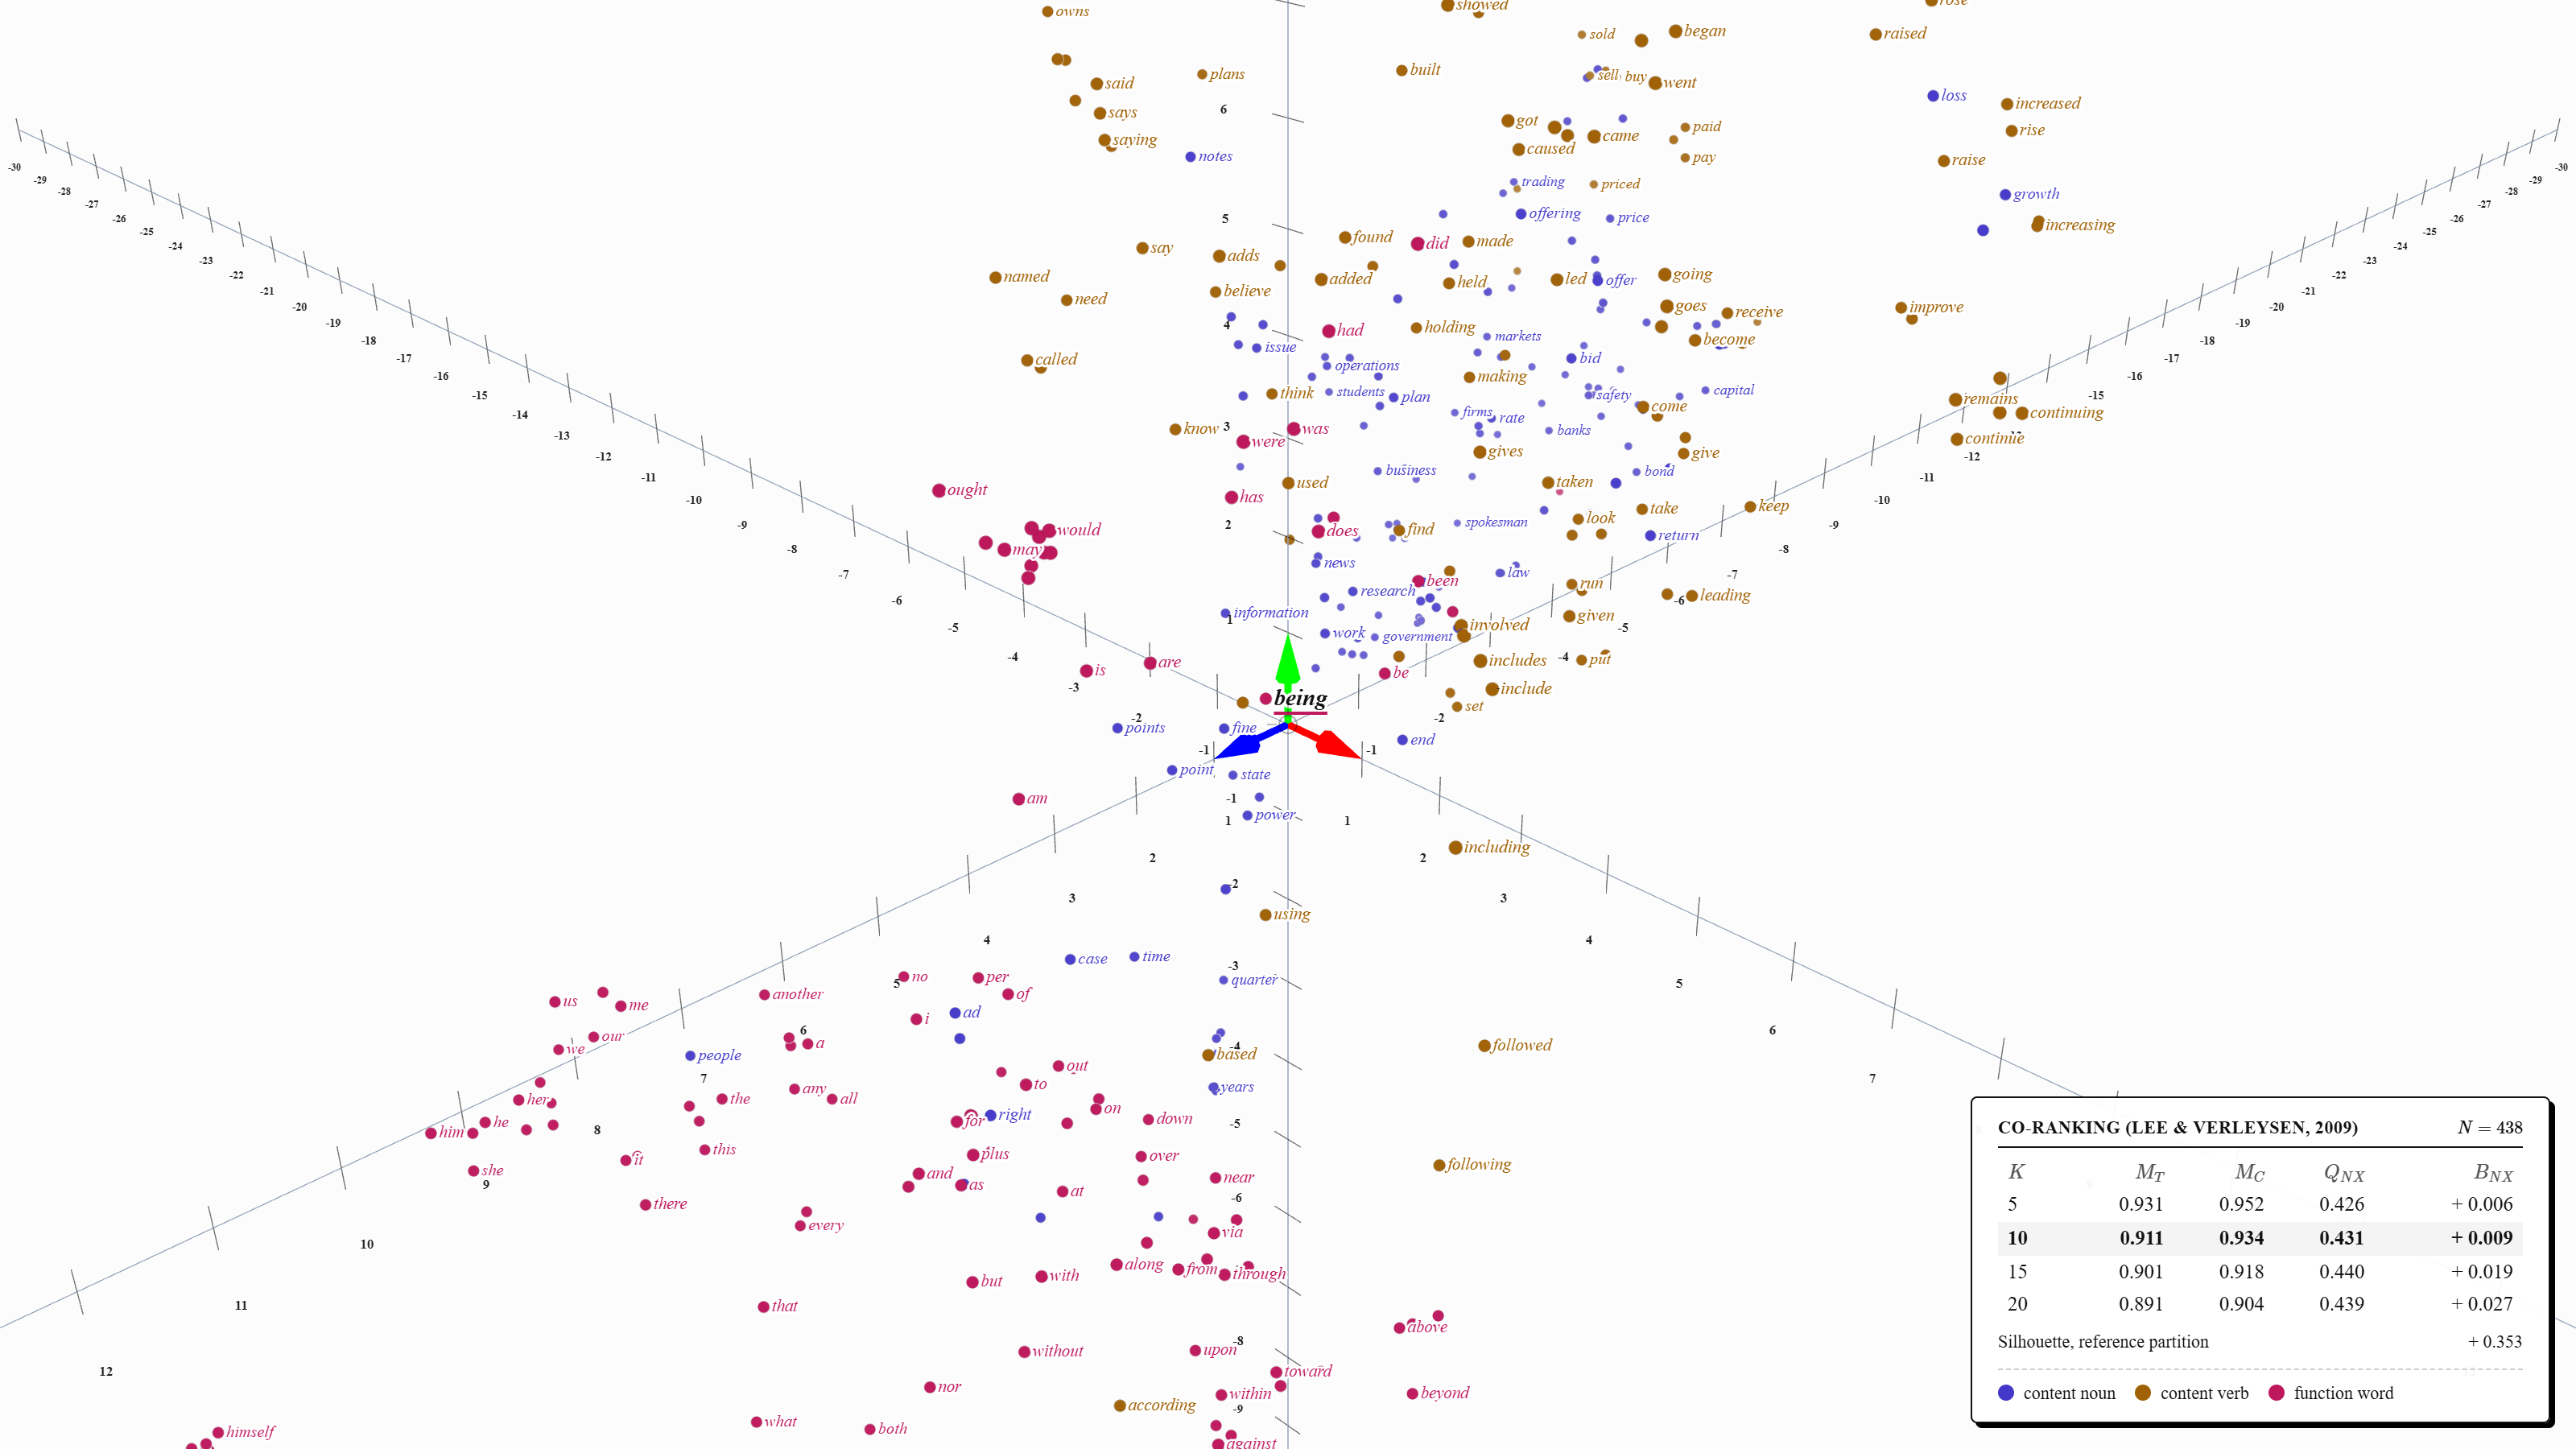
\includegraphics[width=\dimexpr\textwidth-2\fboxrule\relax,frame]{screenshots/fig02_umap.png}
\caption{Gemma 2 2B --- UMAP.}
\label{fig:umap}
\end{figure*}

\begin{figure*}[tp]
\centering
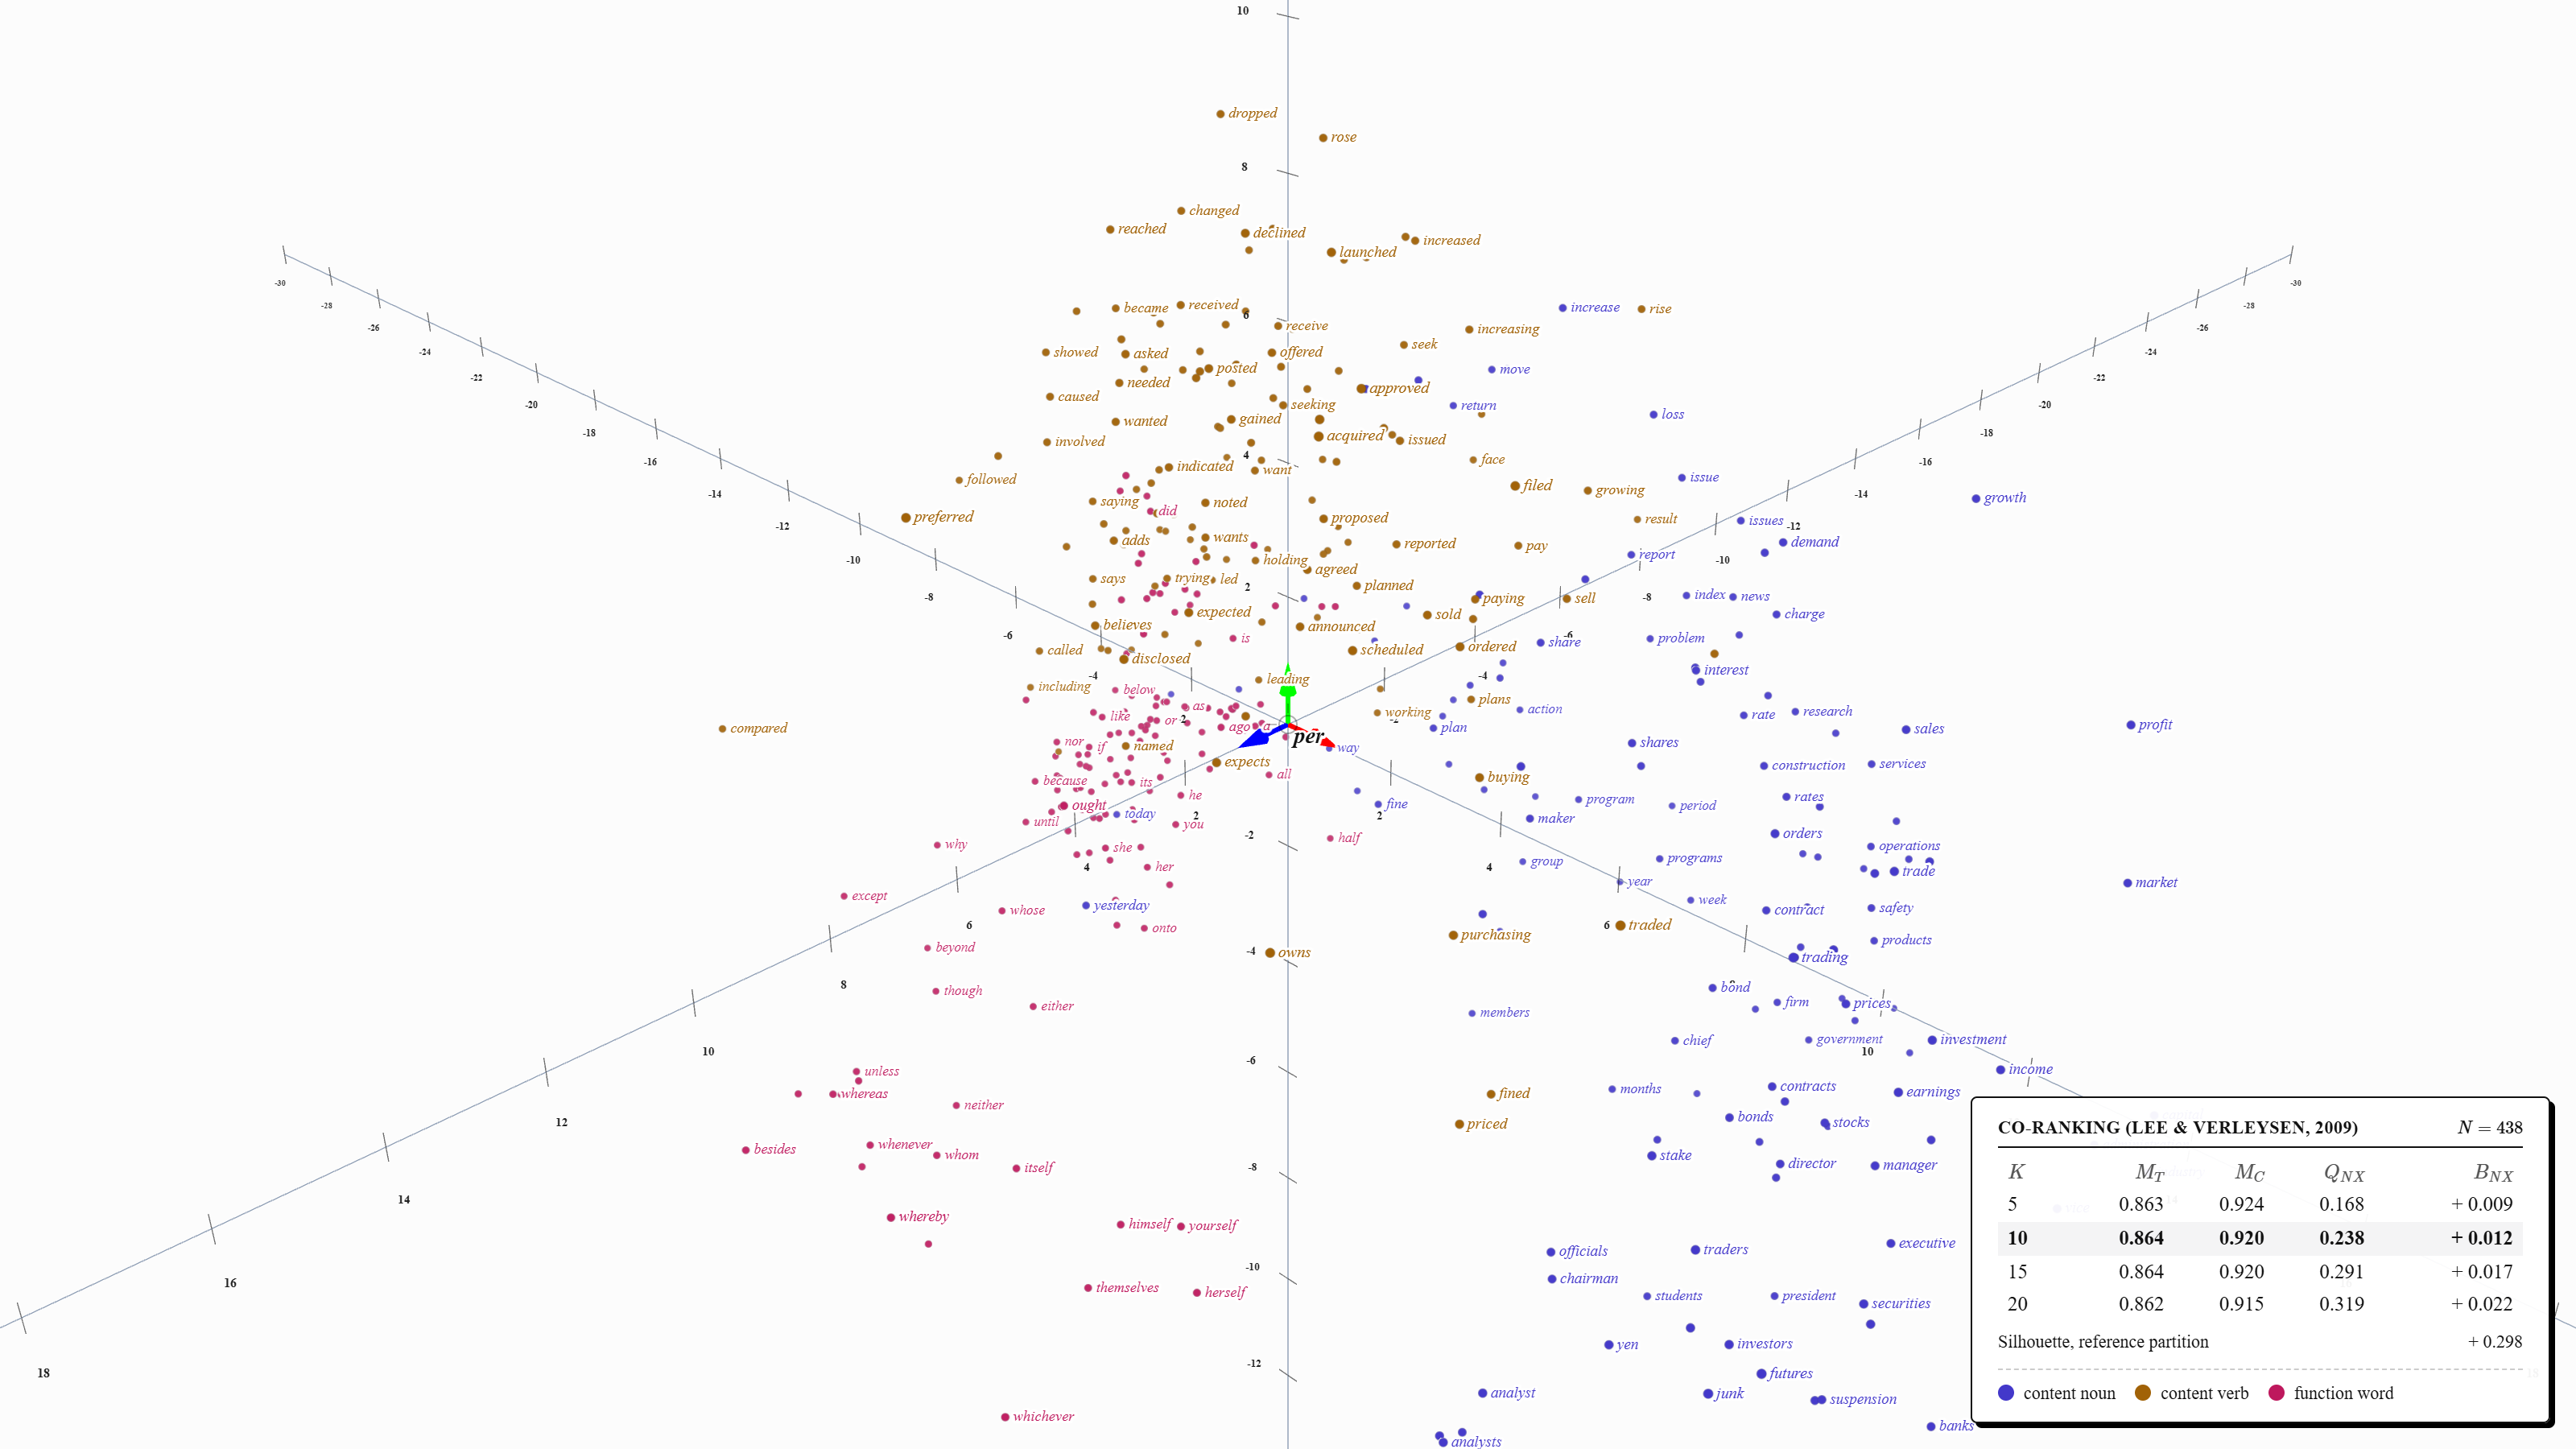
\includegraphics[width=\dimexpr\textwidth-2\fboxrule\relax,frame]{screenshots/fig02_isomap.png}
\caption{Gemma 2 2B --- Isomap.}
\label{fig:isomap}
\end{figure*}

\begin{figure*}[tp]
\centering
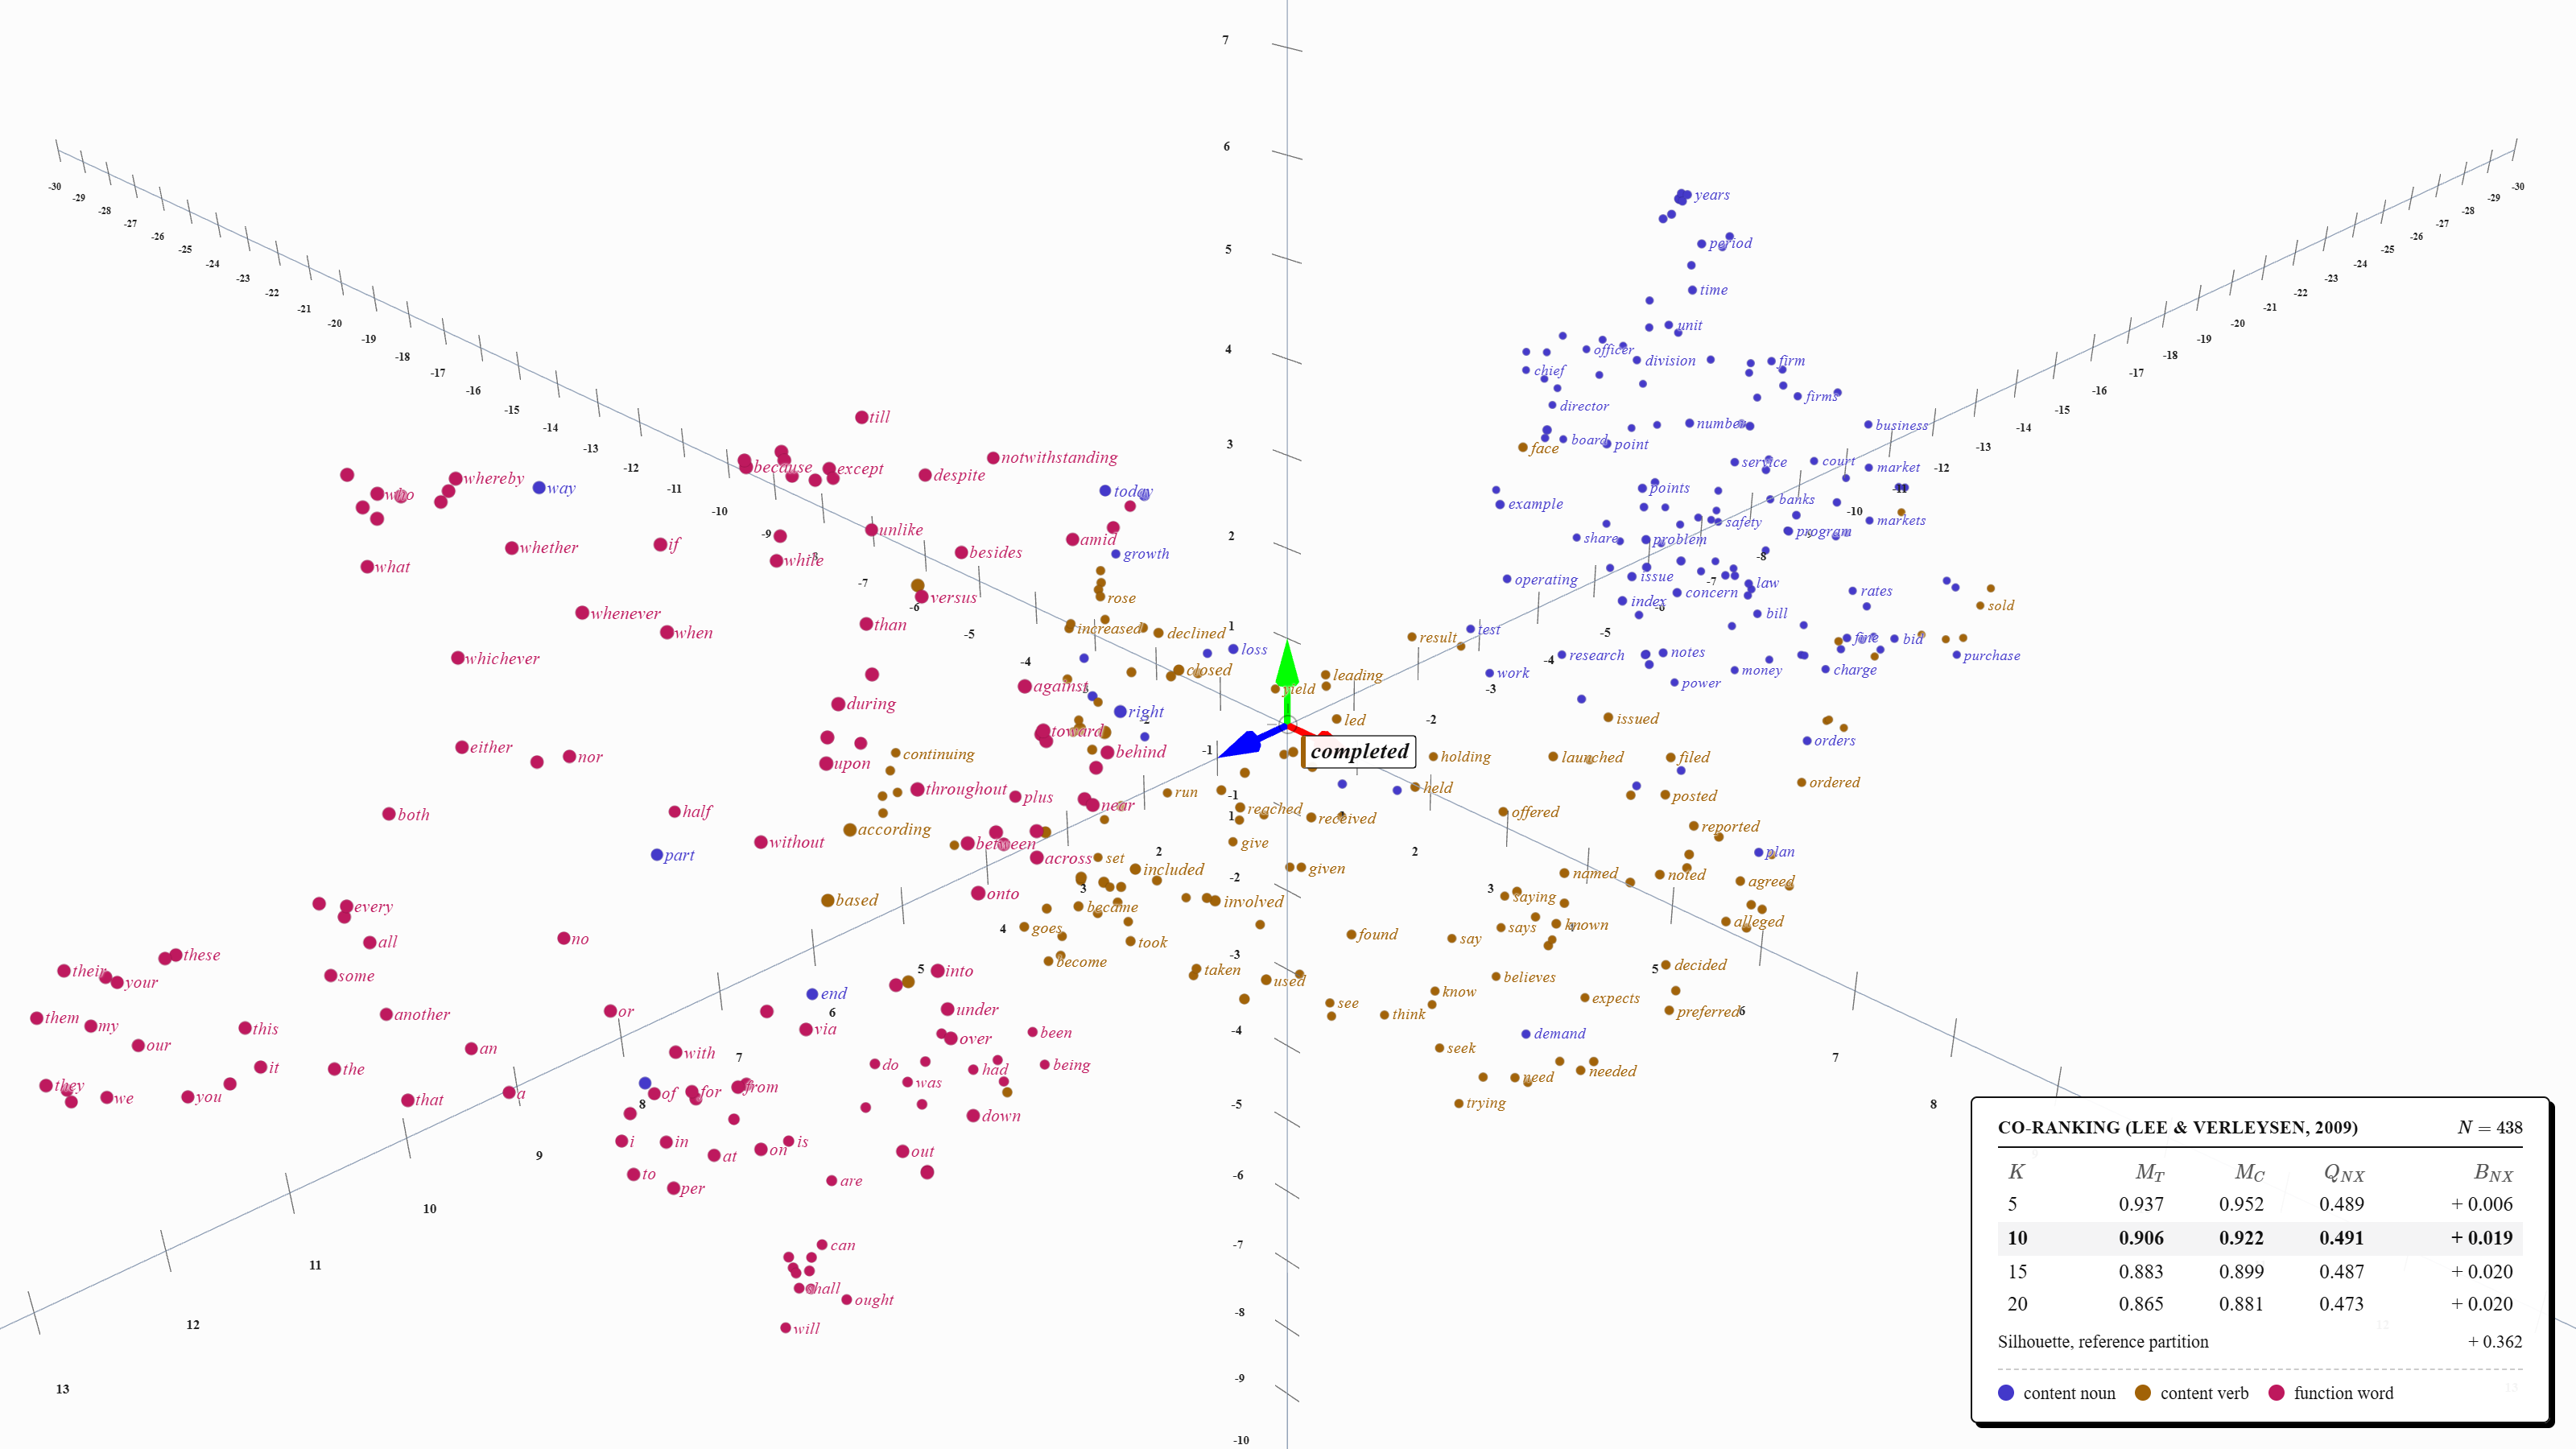
\includegraphics[width=\dimexpr\textwidth-2\fboxrule\relax,frame]{screenshots/fig03_qwen.png}
\caption{Qwen 2.5 0.5B-Instruct --- UMAP.}
\label{fig:qwen}
\end{figure*}

\begin{figure*}[tp]
\centering
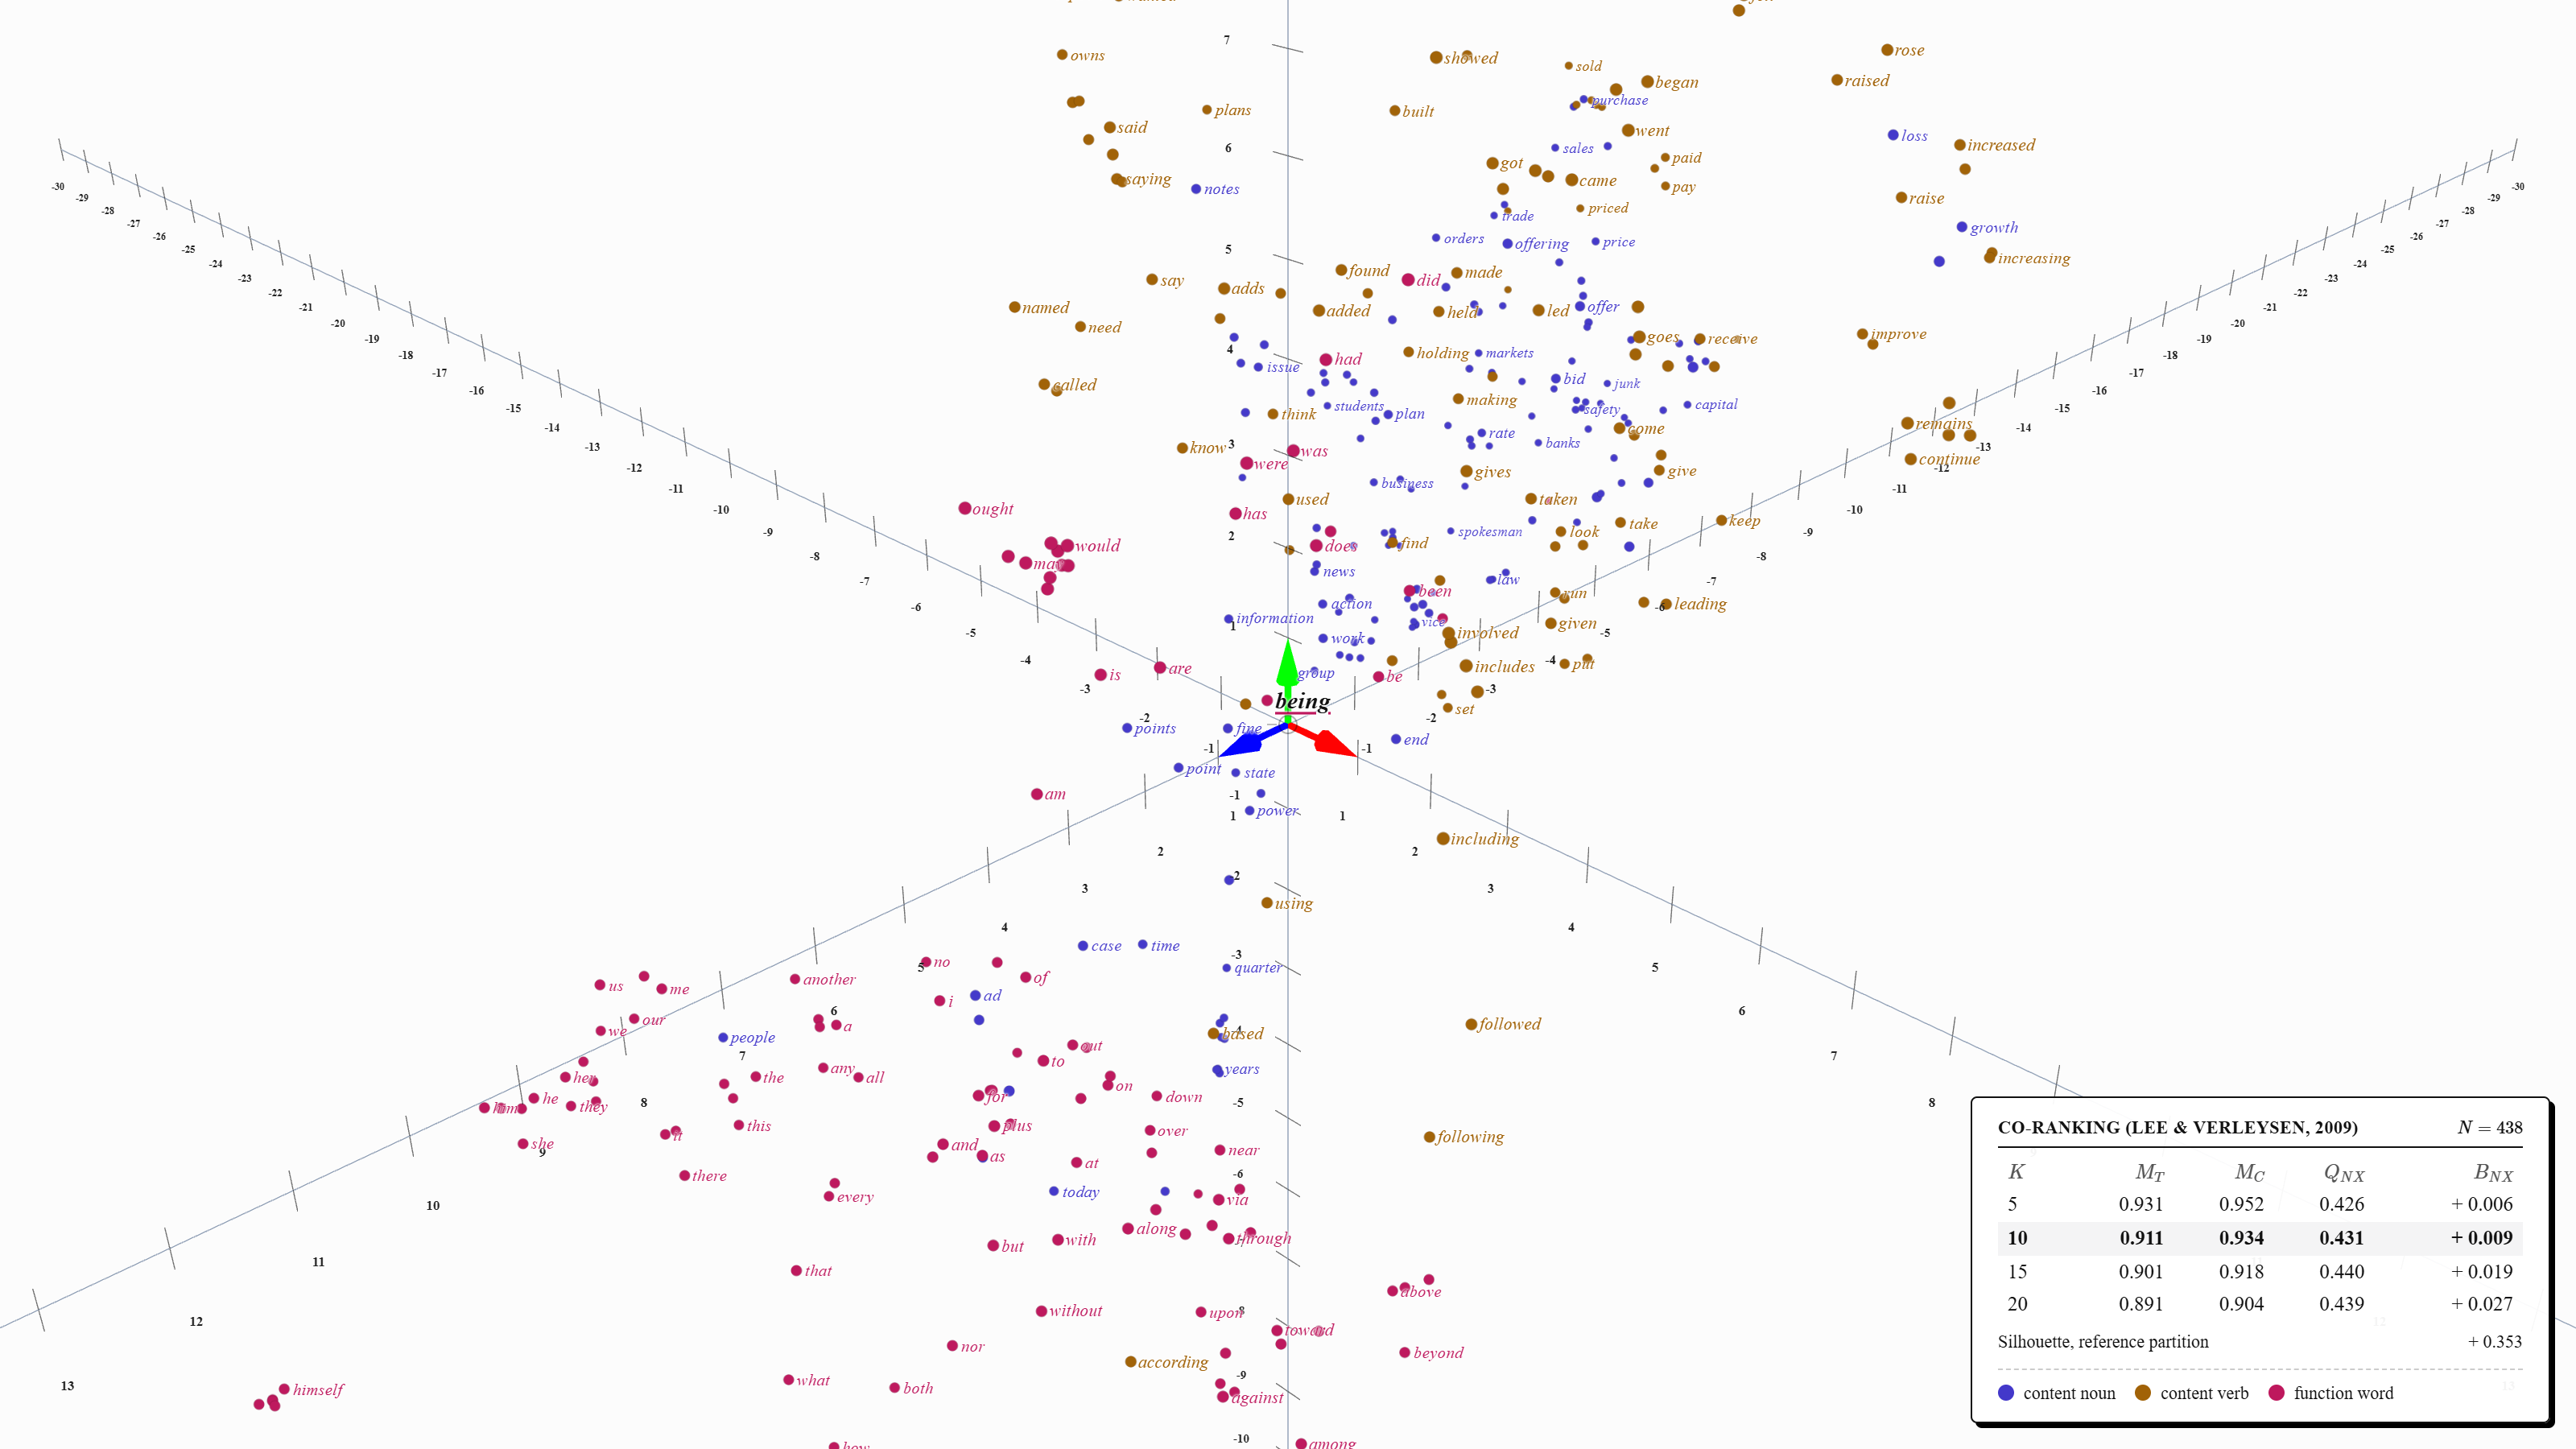
\includegraphics[width=\dimexpr\textwidth-2\fboxrule\relax,frame]{screenshots/fig03_gemma2.png}
\caption{Gemma 2 2B --- UMAP.}
\label{fig:gemma2}
\end{figure*}

\begin{figure*}[tp]
\centering
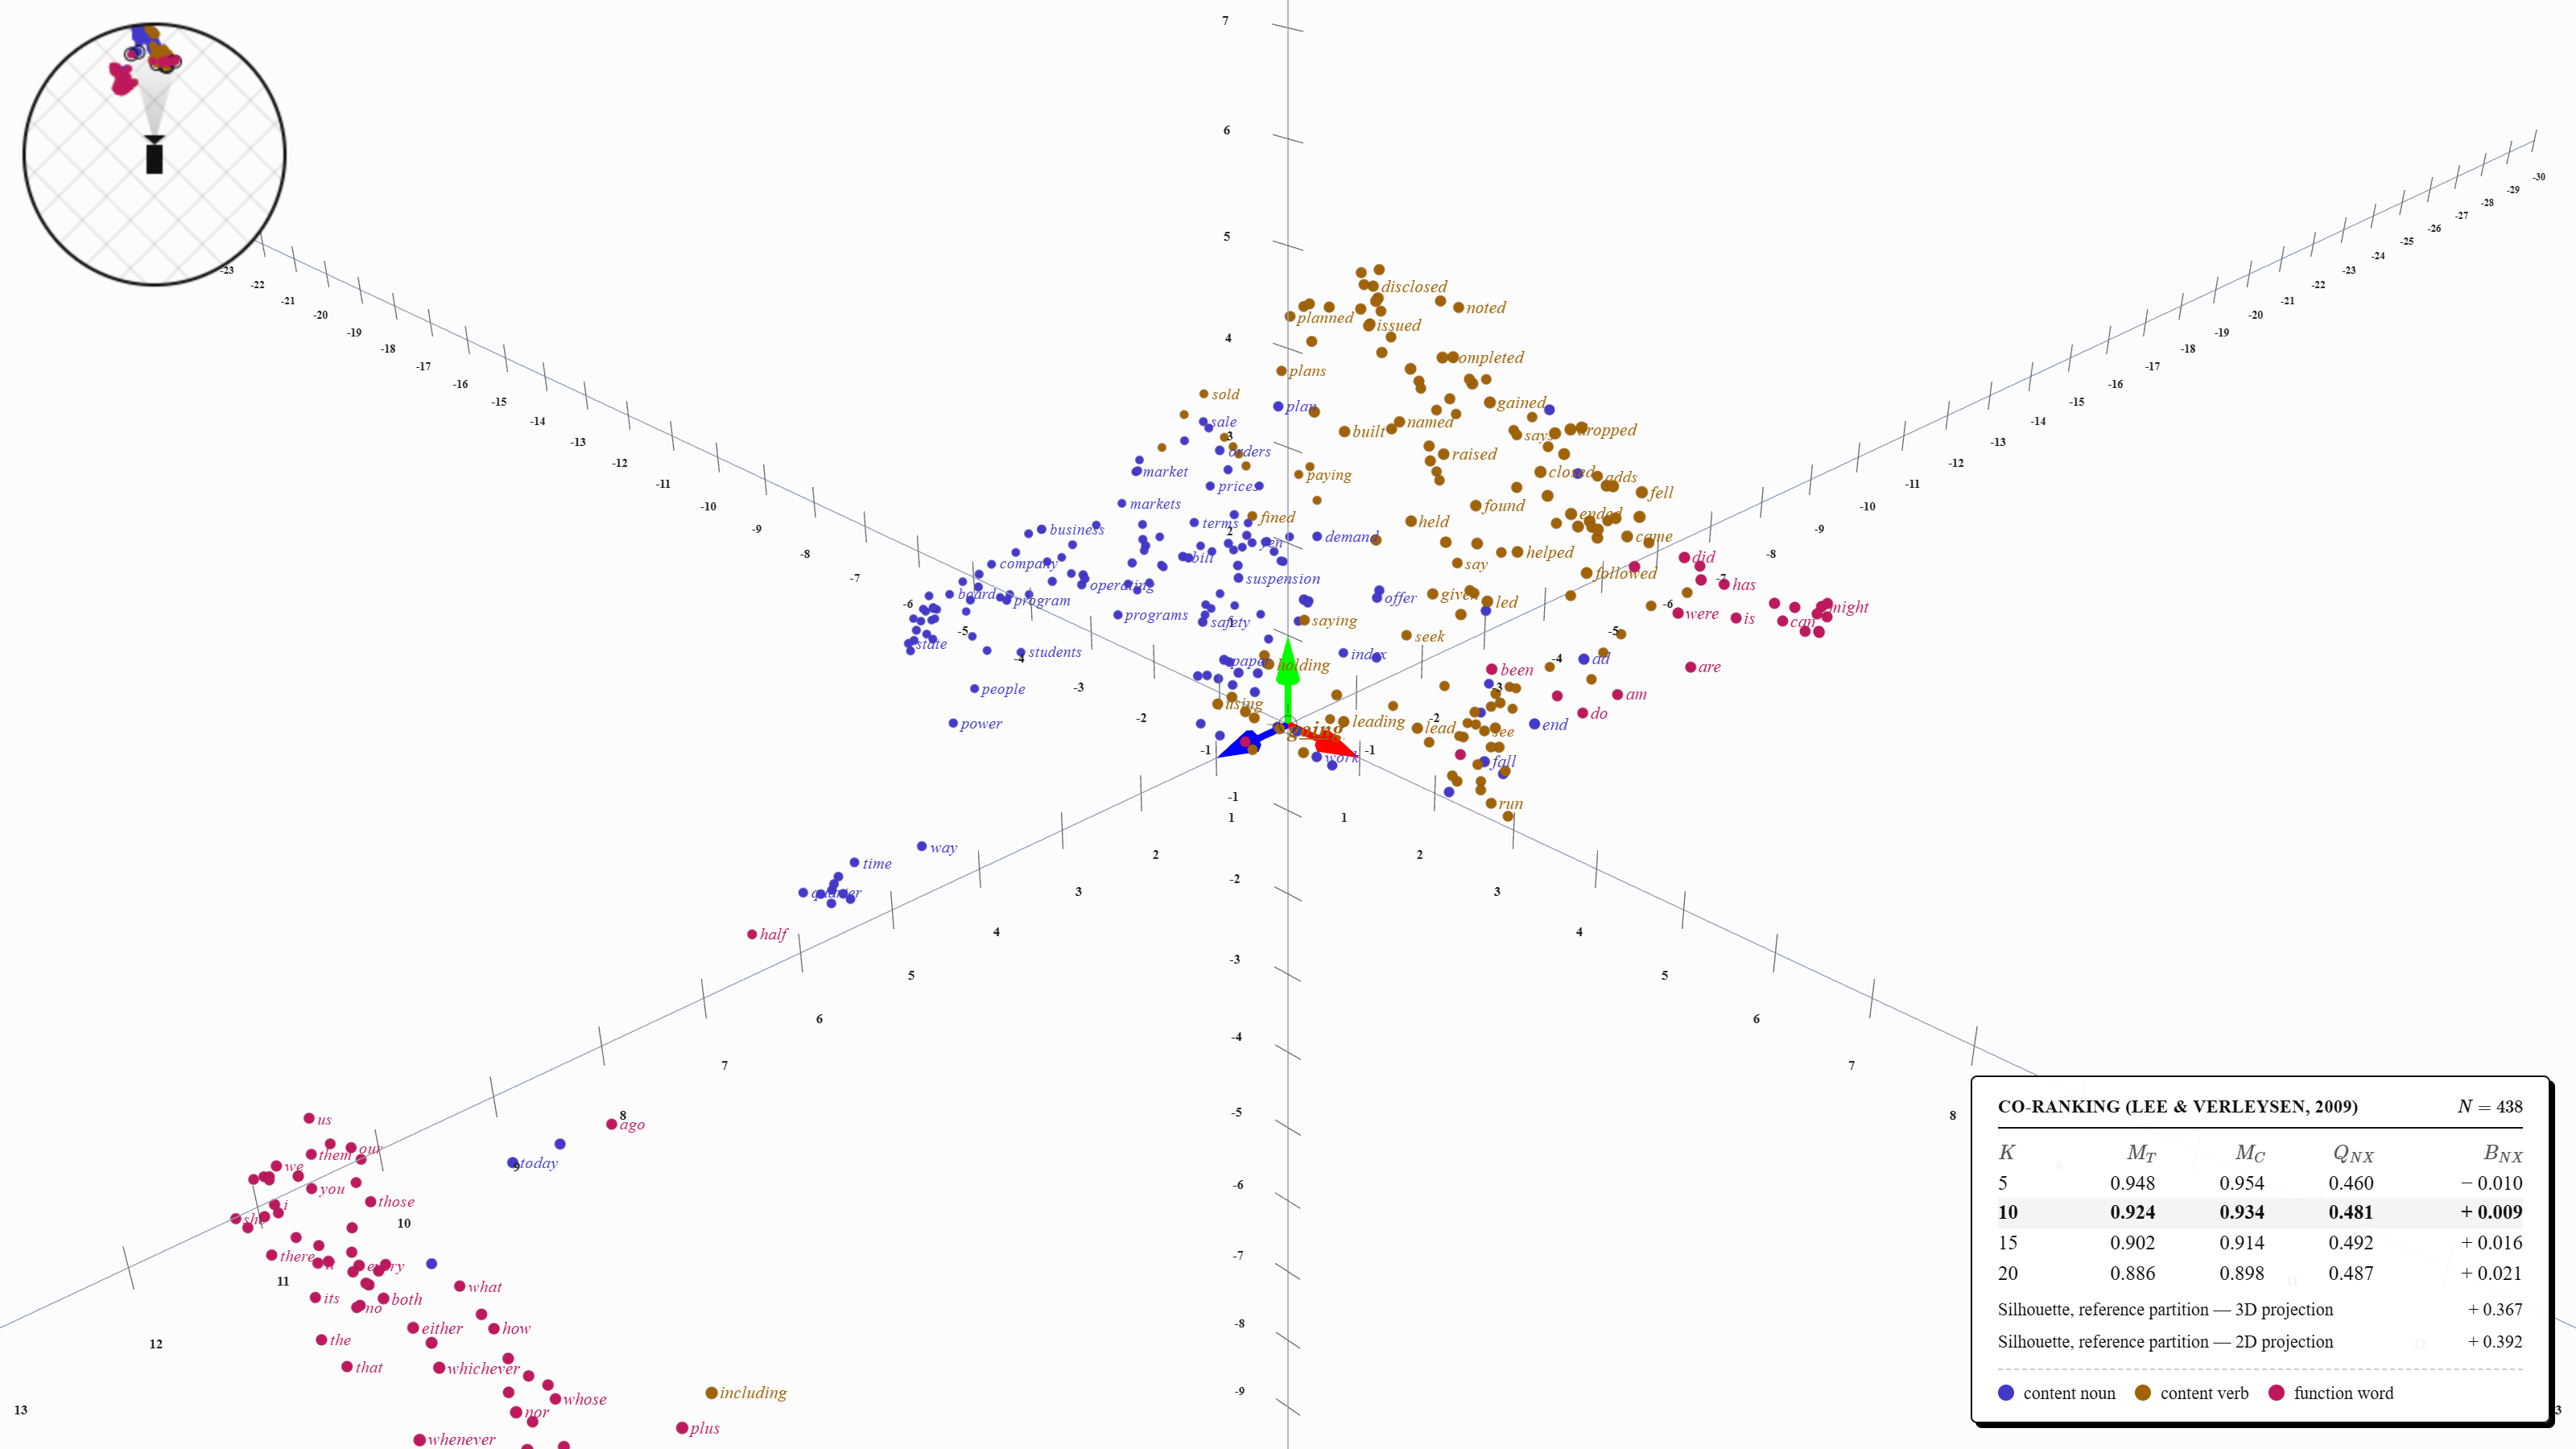
\includegraphics[width=\dimexpr\textwidth-2\fboxrule\relax,frame]{screenshots/fig03_gpt2.png}
\caption{GPT-2 --- UMAP.}
\label{fig:gpt2}
\end{figure*}

\begin{figure*}[tp]
\centering
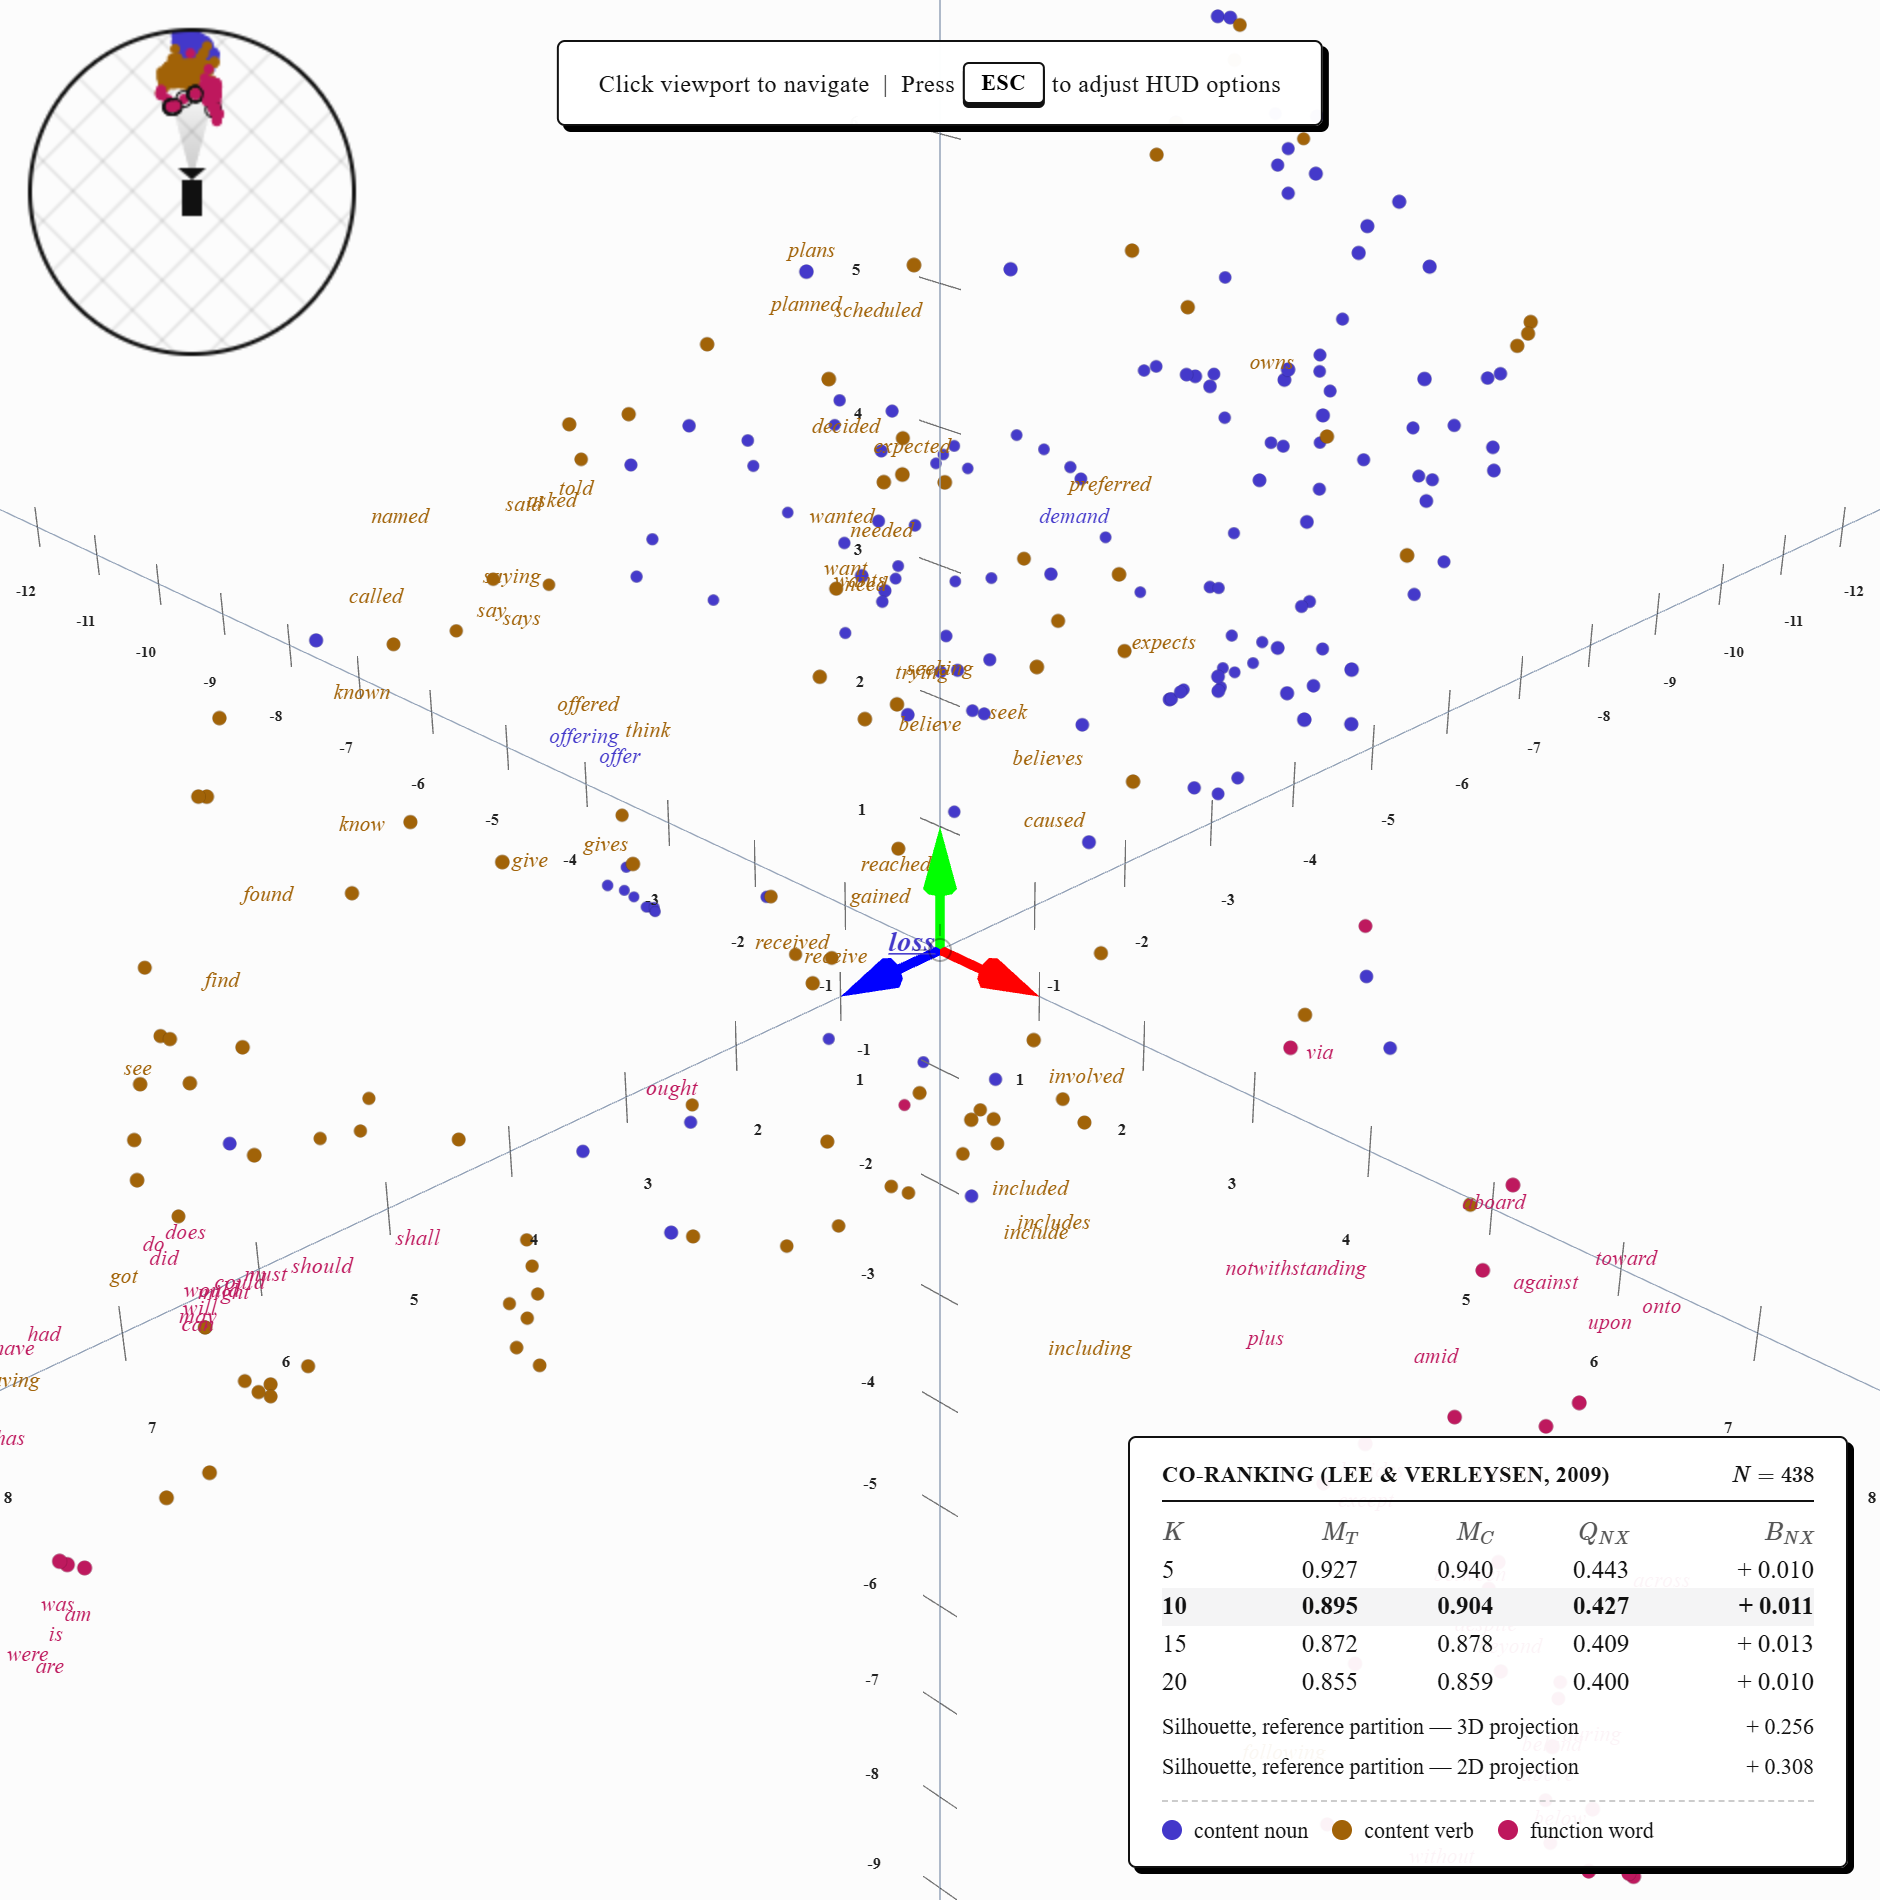
\includegraphics[width=\dimexpr\textwidth-2\fboxrule\relax,frame]{screenshots/fig03_bert.png}
\caption{BERT base uncased --- UMAP.}
\label{fig:bert}
\end{figure*}

\subsection{Sensitivity to seed and perplexity}\label{sec:sensitivity-seed-perplexity}

% BEGIN:sensitivity
\begin{table*}[tp]
\centering
\caption{Sensitivity to Seed and Perplexity at $K = 10$}\label{tab:sensitivity}
\footnotesize
\begin{tabular*}{\textwidth}{@{\extracolsep{\fill}}lllll@{}}
\toprule
Model & Configuration & $M_T(10)$ & $B_{NX}(10)$ & $s$ \\
\midrule
Qwen 2.5 0.5B & t-SNE $p=5$ & 0.878 $\pm$ 0.002 & $+0.012$ $\pm$ 0.003 & $+0.249$ $\pm$ 0.004 \\
Qwen 2.5 0.5B & t-SNE $p=30$ & 0.889 $\pm$ 0.005 & $-0.031$ $\pm$ 0.007 & $+0.185$ $\pm$ 0.028 \\
Qwen 2.5 0.5B & UMAP & 0.904 $\pm$ 0.004 & $+0.028$ $\pm$ 0.005 & $+0.366$ $\pm$ 0.008 \\
GPT-2 & t-SNE $p=5$ & 0.896 $\pm$ 0.002 & $+0.022$ $\pm$ 0.005 & $+0.243$ $\pm$ 0.009 \\
GPT-2 & t-SNE $p=30$ & 0.910 $\pm$ 0.004 & $-0.039$ $\pm$ 0.009 & $+0.207$ $\pm$ 0.022 \\
GPT-2 & UMAP & 0.917 $\pm$ 0.003 & $+0.006$ $\pm$ 0.009 & $+0.365$ $\pm$ 0.009 \\
Gemma 2 2B & t-SNE $p=5$ & 0.883 $\pm$ 0.004 & $+0.018$ $\pm$ 0.006 & $+0.228$ $\pm$ 0.019 \\
Gemma 2 2B & t-SNE $p=30$ & 0.897 $\pm$ 0.003 & $-0.037$ $\pm$ 0.006 & $+0.221$ $\pm$ 0.015 \\
Gemma 2 2B & UMAP & 0.914 $\pm$ 0.002 & $+0.004$ $\pm$ 0.011 & $+0.356$ $\pm$ 0.007 \\
BERT base & t-SNE $p=5$ & 0.879 $\pm$ 0.001 & $-0.002$ $\pm$ 0.003 & $+0.203$ $\pm$ 0.009 \\
BERT base & t-SNE $p=30$ & 0.874 $\pm$ 0.004 & $-0.039$ $\pm$ 0.005 & $+0.181$ $\pm$ 0.019 \\
BERT base & UMAP & 0.891 $\pm$ 0.004 & $+0.017$ $\pm$ 0.006 & $+0.255$ $\pm$ 0.011 \\
\bottomrule
\end{tabular*}
\par\vspace{3pt}\parbox{\textwidth}{\scriptsize \emph{Mean $\pm$ sample standard deviation over seeds \{0, 1, 2, 3, 42\}. Source: \texttt{results/sensitivity\_c2416895b599.json} --- commit \texttt{e7f5a91f} (clean working tree), Python 3.12.14, scikit-learn 1.6.1, umap-learn 0.5.7, seed 42, extraction: HTTP Range rows.}}
\end{table*}
% END:sensitivity

\subsection{Ablation: PCA without centring}\label{sec:ablation-pca-without}

% BEGIN:ablation
\begin{table*}[tp]
\centering
\caption{PCA With and Without Centring}\label{tab:ablation}
\footnotesize
\begin{tabular*}{\textwidth}{@{\extracolsep{\fill}}llll@{}}
\toprule
Model & PCA $M_T$ / $M_C$ & PCA-NC $M_T$ / $M_C$ & PCA-NC $B_{NX}$ \\
\midrule
Qwen 2.5 0.5B & 0.830 / 0.828 & 0.793 / 0.794 & $+0.000$ \\
GPT-2 & 0.827 / 0.846 & 0.761 / 0.799 & $-0.003$ \\
Gemma 2 2B & 0.867 / 0.802 & 0.843 / 0.762 & $-0.008$ \\
BERT base & 0.819 / 0.810 & 0.778 / 0.746 & $-0.009$ \\
\bottomrule
\end{tabular*}
\end{table*}
% END:ablation

\section{Discussion}\label{sec:discussion}

\textbf{The sign of t-SNE's behaviour follows the perplexity.} With the
frozen perplexity of 5, t-SNE is mildly intrusive in three models and
neutral in BERT; with perplexity 30 it is extrusive in all four, and the
gap is many times larger than the spread across five seeds
(Section~\ref{sec:sensitivity-seed-perplexity}). A statement such as ``t-SNE tears the embedding
space'' is therefore a statement about a hyperparameter as much as about
the algorithm. Both values lie in the range recommended by the method's
authors, so neither can be dismissed; the defensible report is the pair.
Low perplexity also showed a numerical artefact: with perplexity 5 a
single word was occasionally ejected far from the cloud, a different one
depending on the seed, although the word was not isolated in the
original space.

\textbf{Projections inflate category separation.} In the original spaces
the reference categories are barely separated (Silhouette 0.025--0.048),
while every projection raises the score above its original-space value,
in most configurations to 0.15--0.40. A visually clean separation of
nouns, verbs and function words in a projection is thus weak evidence
about the embedding space itself; the co-ranking metrics are the
appropriate check.

\textbf{Neighbourhood preservation depends on the algorithm.} UMAP
reaches the highest trustworthiness in every model. Isomap has the
lowest or near-lowest trustworthiness --- below PCA, whose three
components capture only 8--11\% of the variance, in three of the four
models --- but continuity well above it in every model, which \(B_{TC}\)
reports as clearly intrusive (\(+0.057\) to \(+0.117\)).

\textbf{Faithfulness differs between models, independently of
dimension.} Under both t-SNE settings and UMAP, GPT-2 --- the oldest and
smallest of the four models, trained on a different corpus --- has the
highest trustworthiness, and BERT the lowest, although both embed tokens
in 768 dimensions; under PCA, Gemma 2 is highest. Whatever makes an
input-embedding space easier to project faithfully, it is not its
dimension alone. As stated in Section~\ref{sec:models}, the design does not
isolate which property of training is responsible.

\textbf{Two behaviour indicators, two views.} \(B_{NX}\) counts mild
events only; \(B_{TC}\) weights hard events by their rank error. They
can disagree: with perplexity 30, \(B_{NX}\) is negative for t-SNE in
all four models, while the sign of \(B_{TC}\) differs between models.
Reporting both avoids over-reading either.

\subsection{Limitations}\label{sec:limitations}

\textbf{Static embeddings only.} Contextual hidden states are
deliberately out of scope (Section~\ref{sec:input-embeddings-cosine}). \textbf{No causal
attribution.} The models differ in many factors at once.
\textbf{Sample.} The dataset comes from the NLTK sample of the Penn
Treebank and is limited by the 146 function words that are single tokens
in all tokenizers; the results describe these 438 frequent English word
types. \textbf{Descriptive statistics.} The main matrix uses one seed
per configuration; variability is reported by the sensitivity analysis,
and no hypothesis tests are performed. \textbf{Reproducibility across
platforms.} All numbers in Section~\ref{sec:results} come from the
continuous-integration run (Linux, clean checkout of the recorded
commit); two such runs on different commits with unchanged pipeline code
agreed to within \(10^{-6}\). A local re-run on Windows reproduced the
dataset hash and the deterministic projections (PCA, PCA-NC, Isomap)
exactly, but not t-SNE and UMAP: with the same seed, their metrics
differed across the two platforms by amounts comparable to the
seed-to-seed spread of Section~\ref{sec:sensitivity-seed-perplexity}. A fixed seed therefore
guarantees reproducibility only on a fixed software and hardware stack,
and the seed distribution, not a single seed, is the appropriate report
for stochastic projections. \textbf{Single-tokenisation bias.}
Restricting to single-token words favours frequent, short words, whose
embeddings are typically better trained.

\section{Conclusion}\label{sec:conclusion}

ENSy turns the projection of an embedding matrix from a picture into a
measurement. Its co-ranking implementation is validated against an
independent library, synthetic permutations and the primary source, and
its results are regenerated from a frozen dataset by a pinned pipeline.
Applied to four language models, it shows that the visual impressions
most often drawn from such projections --- whether a method crowds or
tears the space, and whether linguistic categories form clusters ---
depend strongly on the projection and its hyperparameters. Projections
of embedding spaces should therefore be reported with their
neighbourhood-preservation metrics and their hyperparameters, never
alone. Natural extensions are contextual representations, larger and
multilingual samples, and inferential statistics over seeds and samples.

\appendices

\section{Reproducing the results}\label{sec:app-reproducing}

Every step runs from the repository root; \texttt{<hash>} is the dataset
hash prefix.
\begin{enumerate}
\item \texttt{pip install -r requirements.txt} --- pinned versions.
\item \texttt{export HF\_TOKEN=...} --- a token whose account accepted the
  licence of \texttt{google/gemma-2-2b}.
\item \texttt{python -m ensy.dataset} --- rebuilds \texttt{data/dataset.json};
  the hash must match.
\item \texttt{python -m ensy.experiment} --- the main matrix, written to
  \texttt{results/main\_\textless{}hash\textgreater{}.json}.
\item \texttt{python -m ensy.experiment -{}-ablation} --- PCA-NC, written to
  \texttt{results/ablation\_\textless{}hash\textgreater{}.json}.
\item \texttt{python -m ensy.experiment -{}-sensitivity} --- seeds and
  perplexity, written to \texttt{results/sensitivity\_\textless{}hash\textgreater{}.json}.
\item \texttt{python -m ensy.compare A.json B.json -{}-markdown} --- compares
  two runs of the main matrix.
\item \texttt{python docs/update\_results.py} --- regenerates the tables and
  plots of Section~\ref{sec:results}.
\item \texttt{python docs/capture\_screenshots.py} --- regenerates the
  screenshots (server running).
\item \texttt{python docs/build\_pdf.py} --- builds this PDF from
  \texttt{docs/DOCS.tex}.
\end{enumerate}

\section{Additional views}\label{sec:app-views}

\begin{figure*}[tp]
\centering
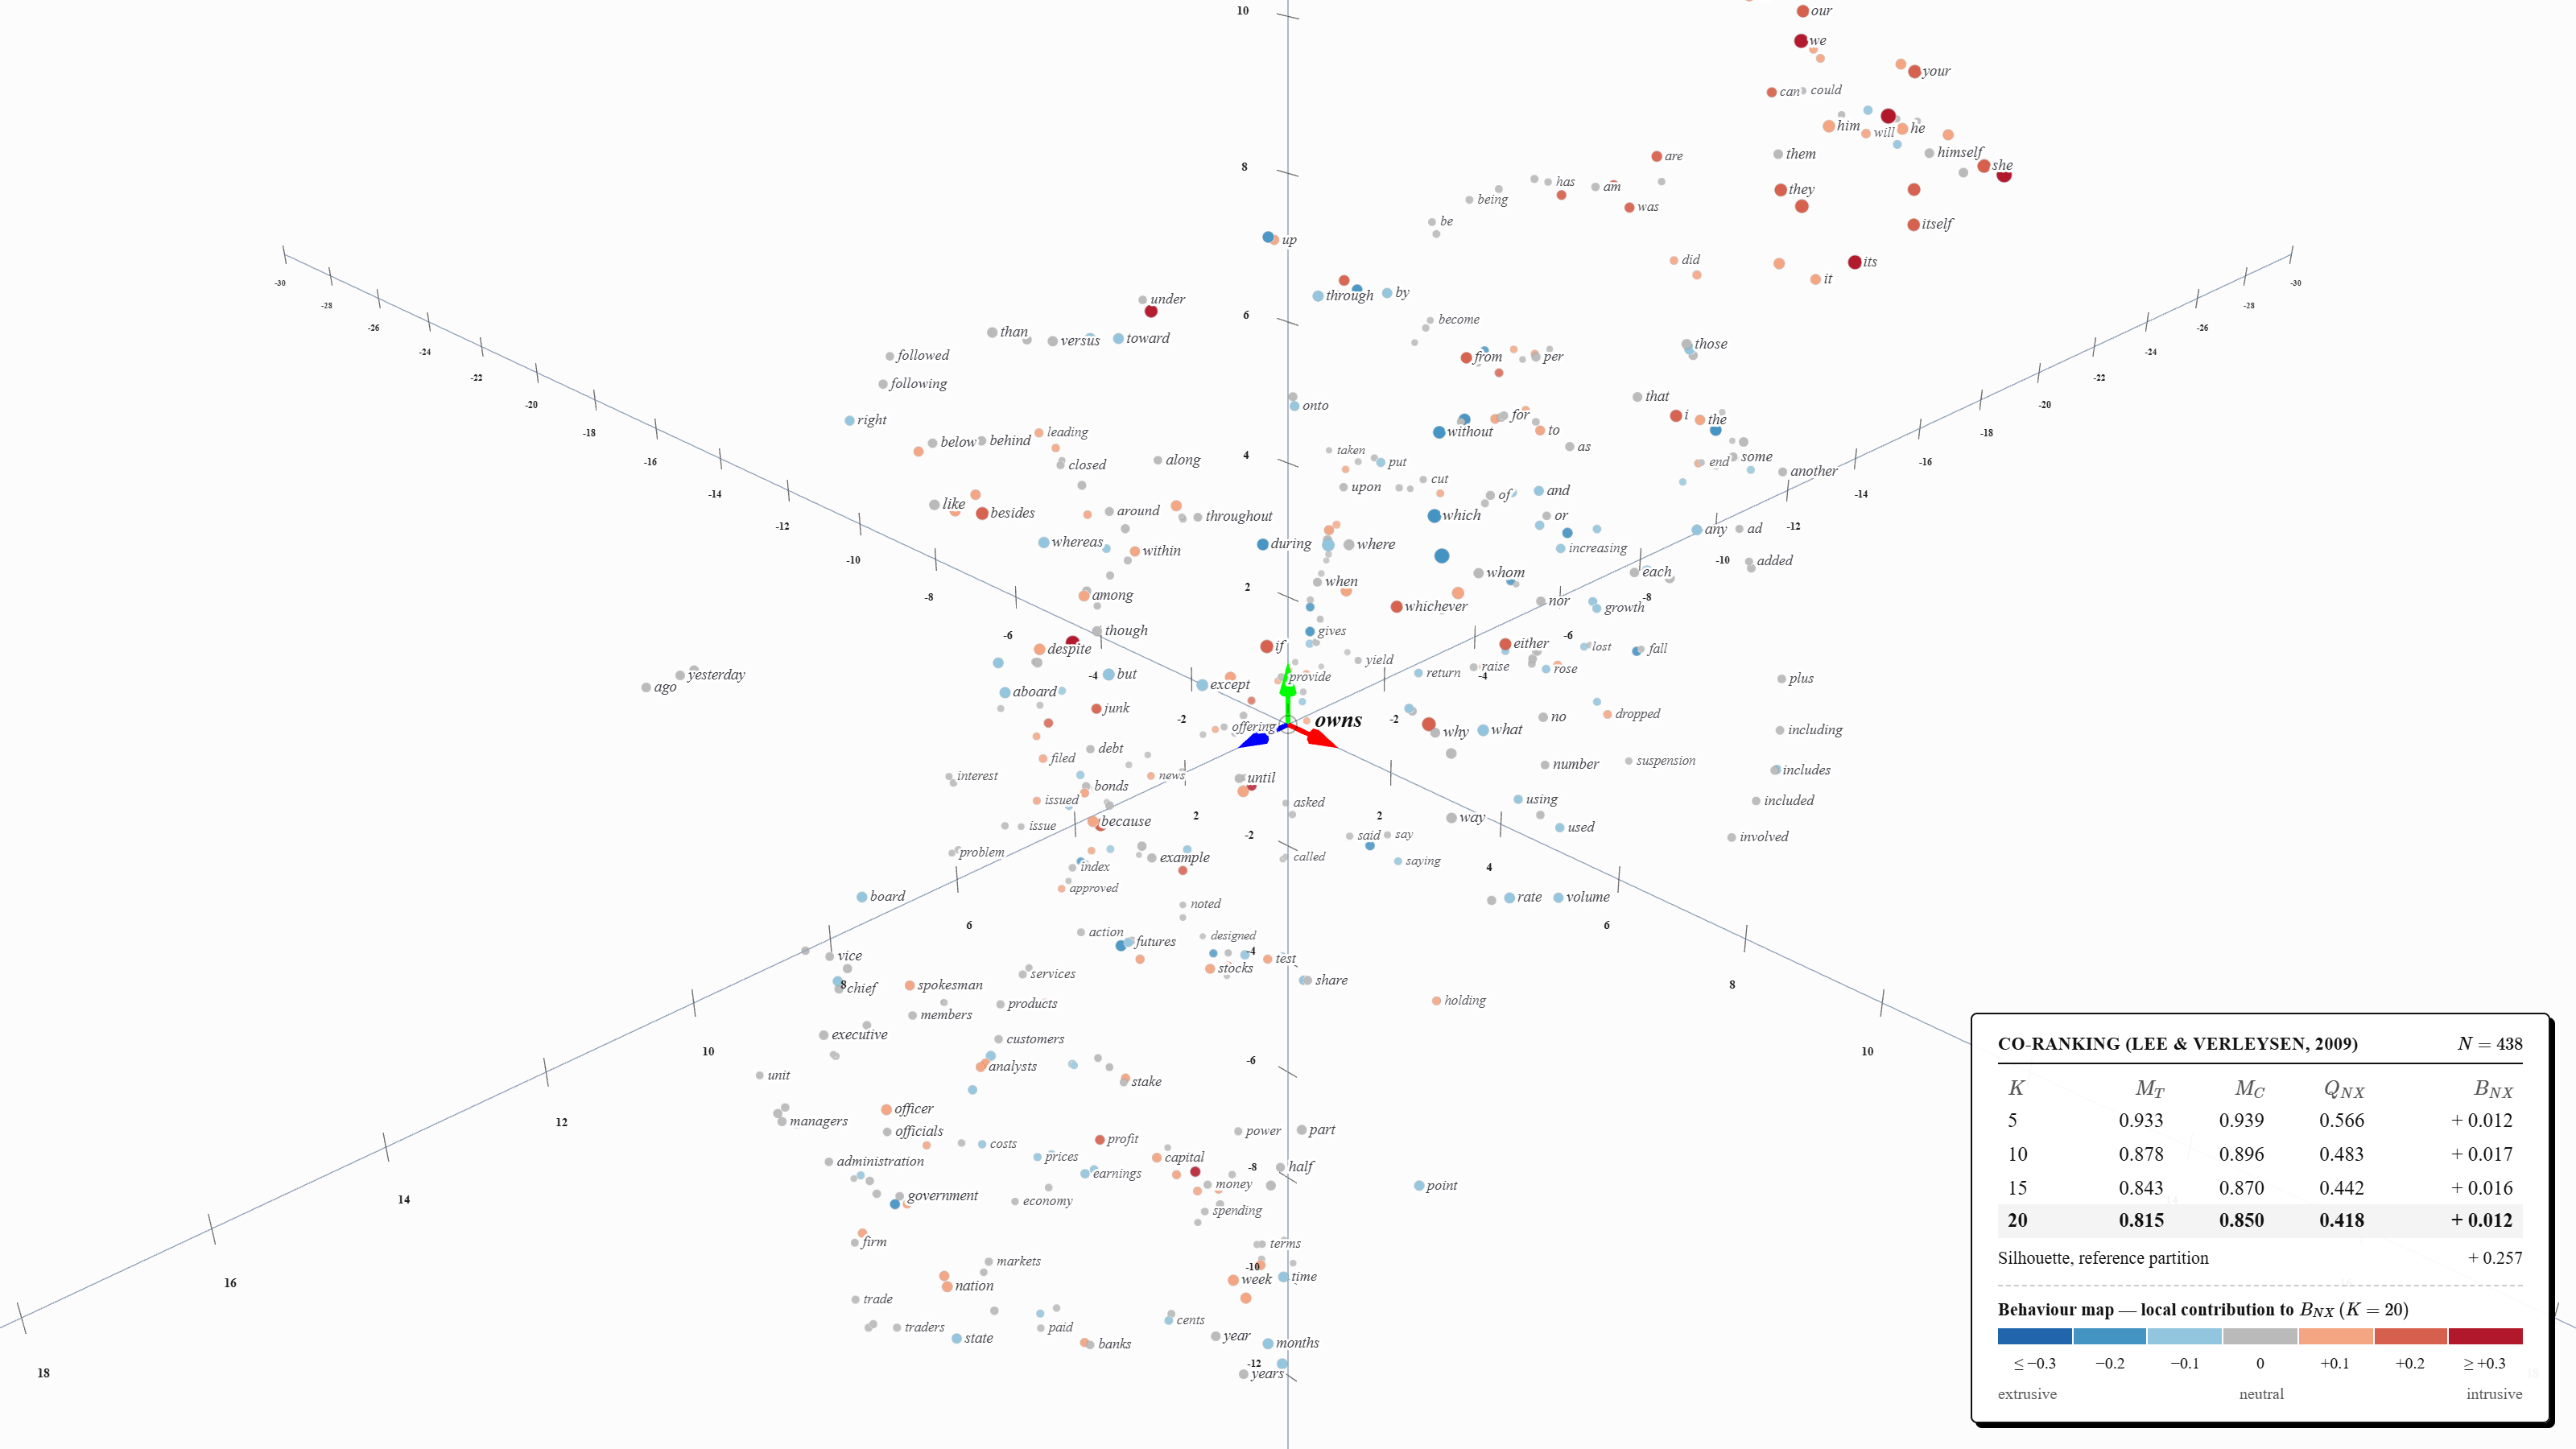
\includegraphics[width=\dimexpr\textwidth-2\fboxrule\relax,frame]{screenshots/fig05_behaviour_k20.png}
\caption{Behaviour map for the same projection as Fig.~\ref{fig:behaviour-k10} at \(K = 20\).}
\label{fig:behaviour-k20}
\end{figure*}

\begin{figure*}[tp]
\centering
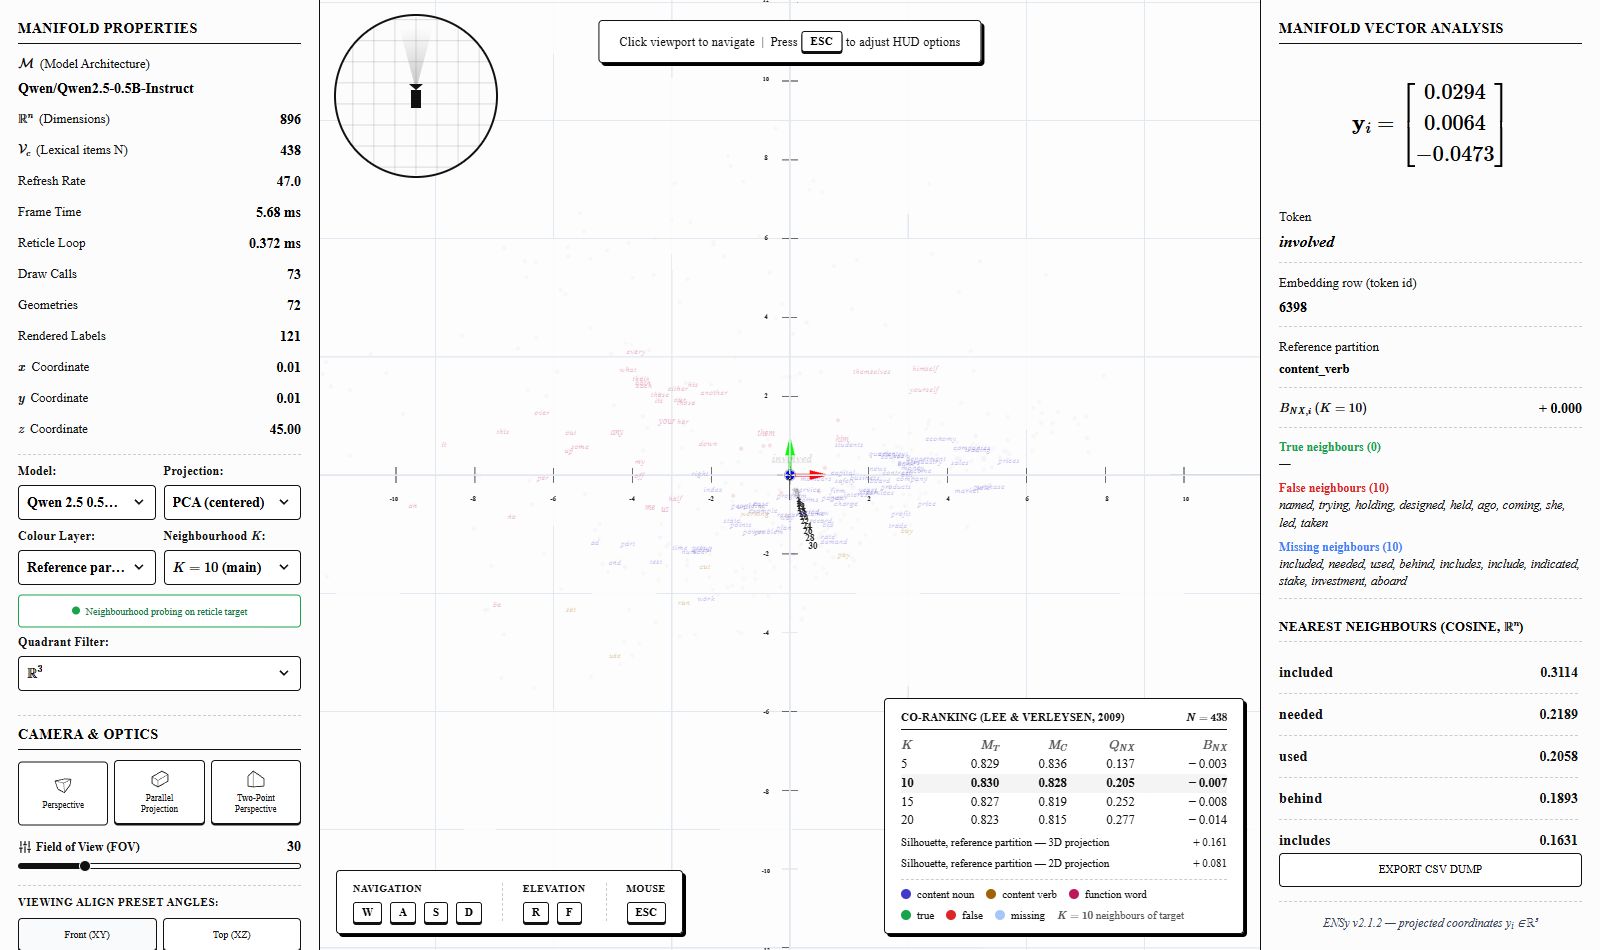
\includegraphics[width=\dimexpr\textwidth-2\fboxrule\relax,frame]{screenshots/fig11_front.png}
\caption{Front (XY) camera preset with the parallel (orthographic) camera on the
PCA projection of Qwen 2.5; grid-plane backgrounds off.}
\label{fig:front}
\end{figure*}

\begin{figure*}[tp]
\centering
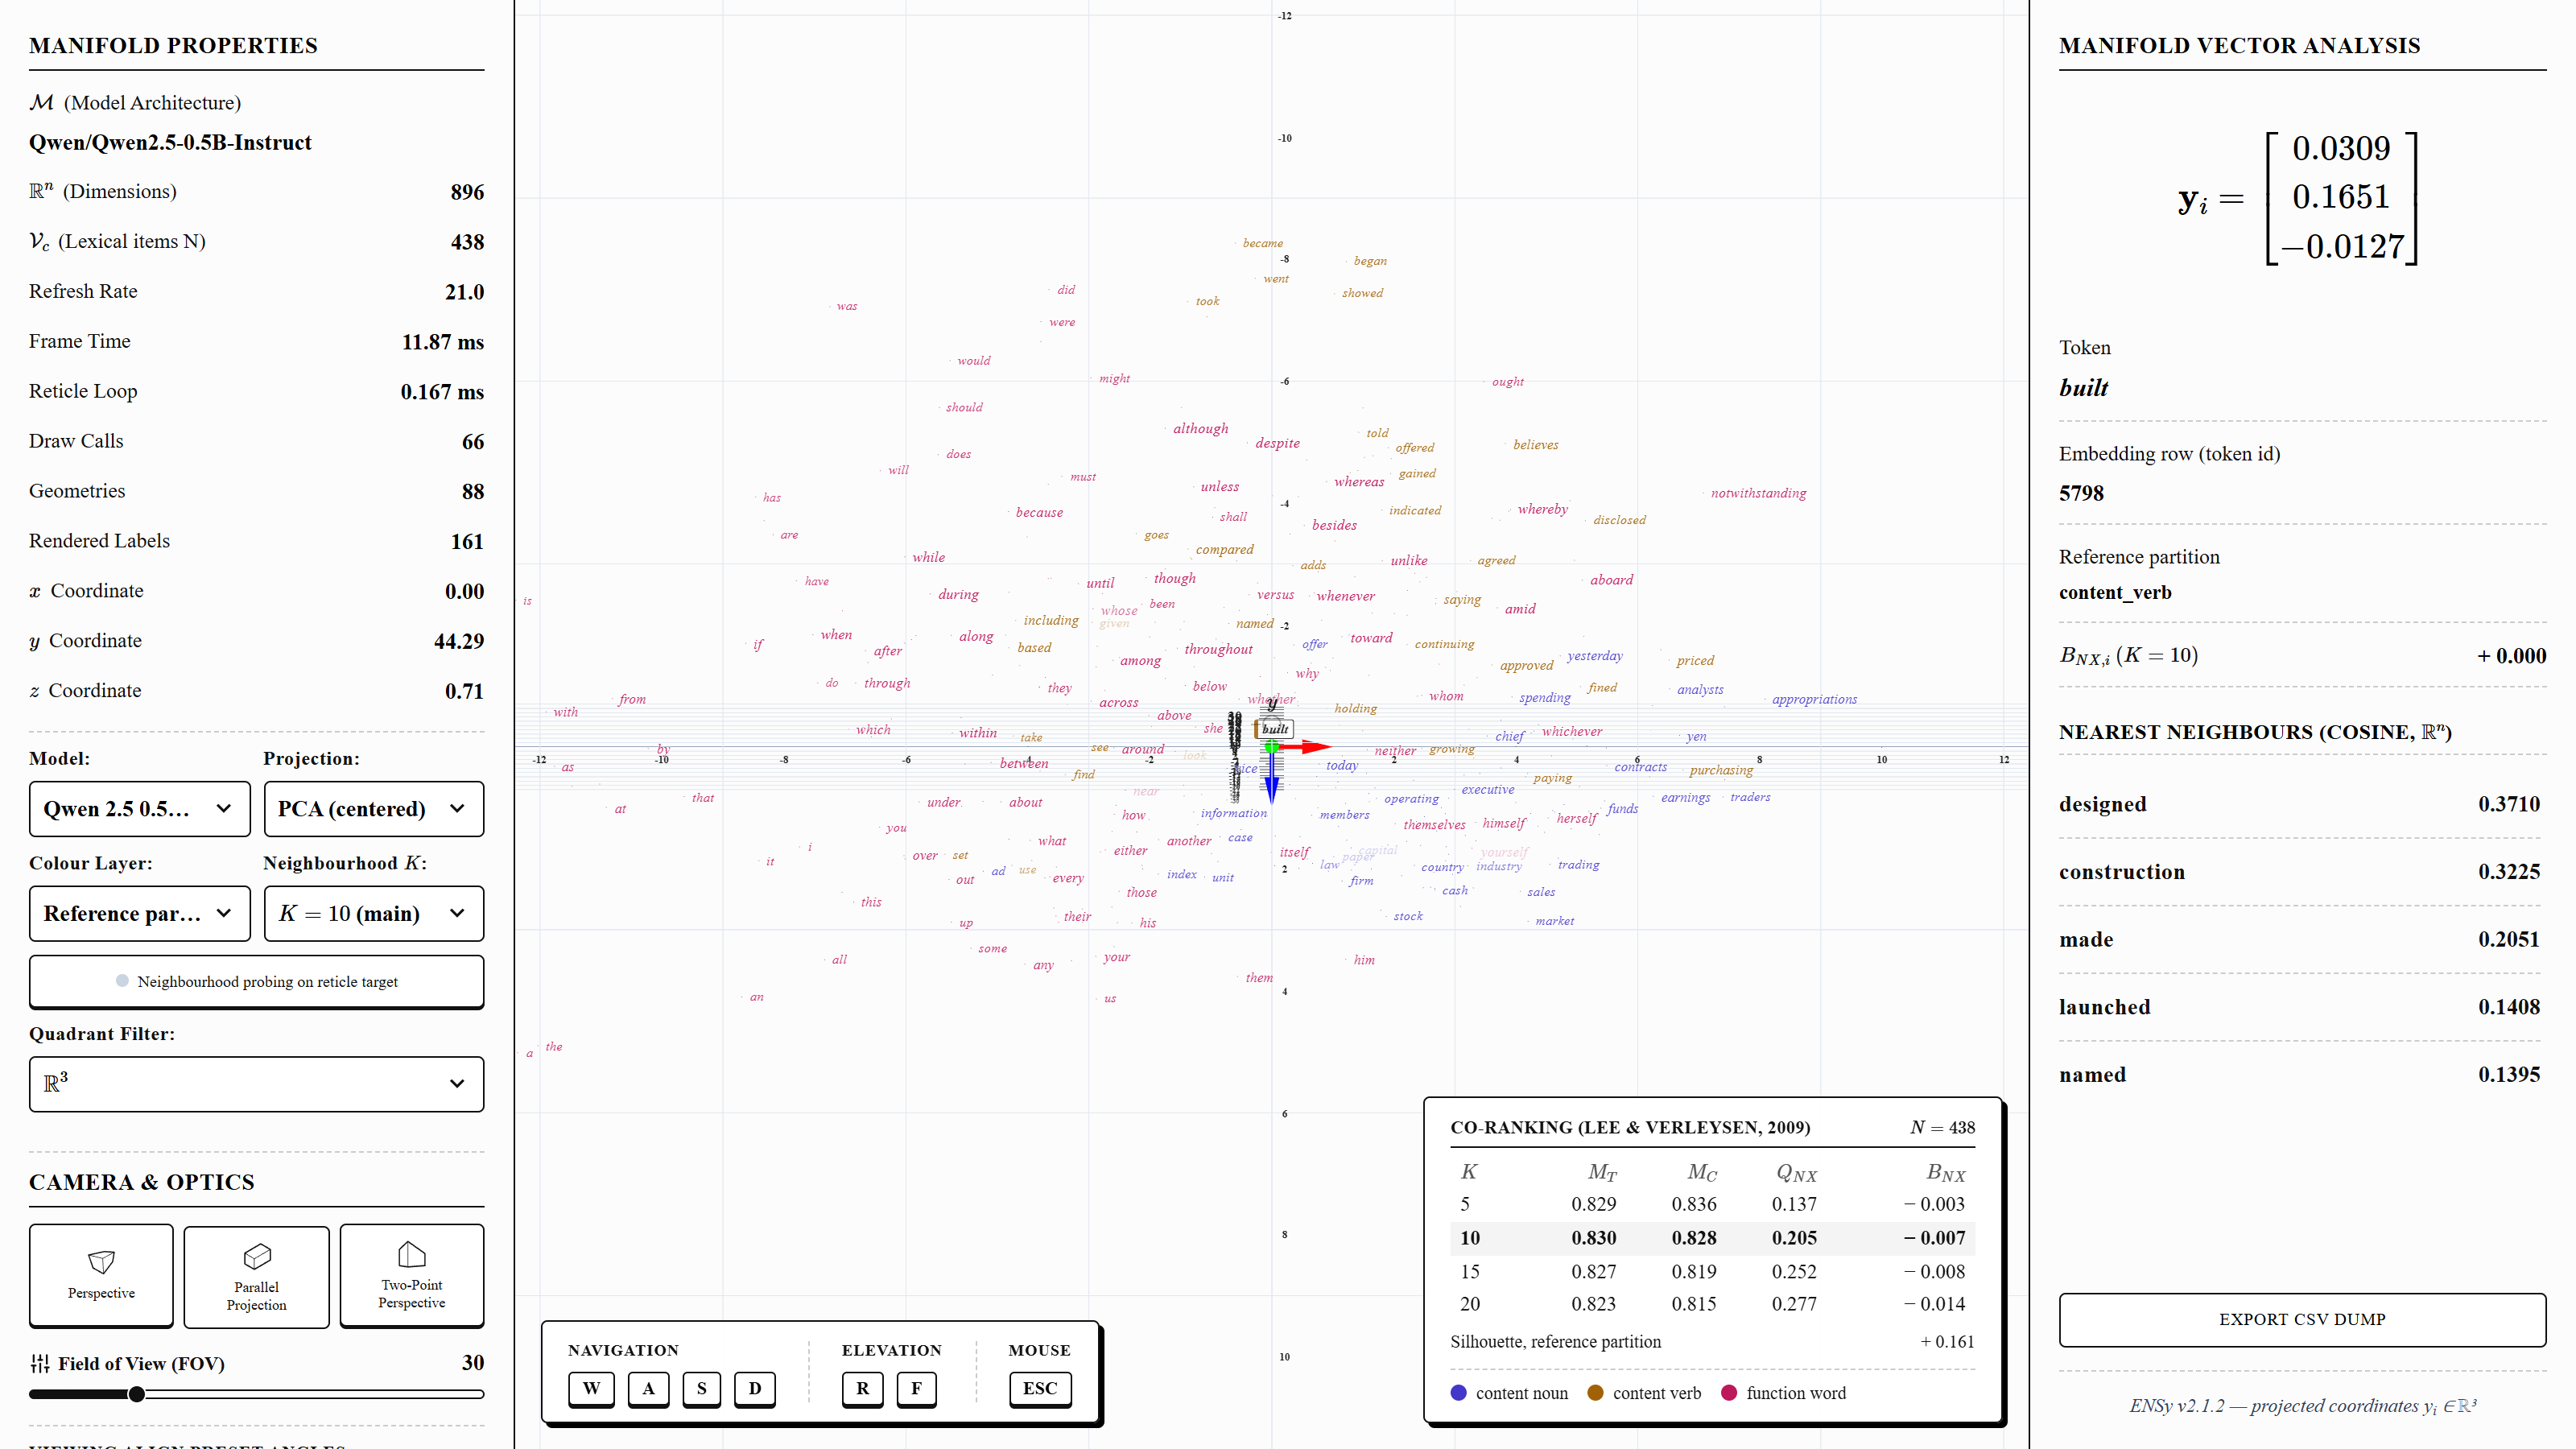
\includegraphics[width=\dimexpr\textwidth-2\fboxrule\relax,frame]{screenshots/fig12_top.png}
\caption{Top (XZ) camera preset with the parallel (orthographic) camera on the
PCA projection of Qwen 2.5; grid-plane backgrounds off.}
\label{fig:top}
\end{figure*}

\section{API}\label{sec:app-api}

\begin{table}[tp]
\centering
\caption{REST Endpoints}\label{tab:rest-endpoints}
\footnotesize
\begin{tabularx}{\columnwidth}{>{\raggedright\arraybackslash}X>{\raggedright\arraybackslash}X}
\toprule
Endpoint & Description \\
\midrule
\path|GET /api/health| & dataset path, \(N\), frozen flag \\
\path|GET /api/models| & models, gating, whether the dataset covers them \\
\path|GET /api/dataset| & dataset metadata and items \\
\path|POST /api/dataset| & rebuild the dataset (refuses to overwrite a frozen one without
\path|force|) \\
\path|GET /api/projection/{model}/{algorithm}| & coordinates, metric curves, \(B_{NX,i}(K)\), neighbour lists, Silhouette
(3D; a 2D value is also served) \\
\path|GET /api/compare| & metric curves of every configuration of the main matrix \\
\bottomrule
\end{tabularx}
\end{table}

\texttt{model} ∈ \{\texttt{qwen}, \texttt{gemma2}, \texttt{gpt2},
\texttt{bert}\}; \texttt{algorithm} ∈ \{\texttt{pca}, \texttt{pca\_nc},
\texttt{tsne}, \texttt{tsne\_p30}, \texttt{umap}, \texttt{isomap}\}.

\section{Keyboard controls}\label{sec:app-keyboard}

\begin{table}[tp]
\centering
\caption{Keyboard Controls}\label{tab:keyboard-controls}
\footnotesize
\begin{tabularx}{\columnwidth}{l>{\raggedright\arraybackslash}X}
\toprule
Input & Action \\
\midrule
Click viewport & engage pointer lock (flight mode) \\
W / S & fly forward / backward along the aim direction (towards the reticle) \\
A / D & strafe left / right \\
R / F & move up / down \\
Mouse & look (pitch clamped) \\
Wheel & zoom \\
H & toggle the navigation HUD \\
Esc & release pointer lock \\
\bottomrule
\end{tabularx}
\end{table}

\begin{thebibliography}{99}
\bibitem{r1} J. A. Lee and M. Verleysen, ``Quality assessment of dimensionality
reduction: Rank-based criteria,'' \emph{Neurocomputing}, vol.~72, no.
7--9, pp.~1431--1443, 2009.
\bibitem{r2} T. Mikolov, K. Chen, G. Corrado, and J. Dean, ``Efficient estimation of
word representations in vector space,'' in \emph{Proc. Int. Conf. Learn.
Represent. (ICLR) Workshop}, 2013, arXiv:1301.3781.
\bibitem{r3} L. G. Nonato and M. Aupetit, ``Multidimensional projection for visual
analytics: Linking techniques with distortions, tasks, and layout
enrichment,'' \emph{IEEE Trans. Vis. Comput. Graphics}, vol.~25, no. 8,
pp.~2650--2673, 2019.
\bibitem{r4} K. Ethayarajh, ``How contextual are contextualized word representations?
Comparing the geometry of BERT, ELMo, and GPT-2 embeddings,'' in
\emph{Proc. EMNLP-IJCNLP}, Hong Kong, China, 2019, pp.~55--65.
\bibitem{r5} X. Cai, J. Huang, Y. Bian, and K. Church, ``Isotropy in the contextual
embedding space: Clusters and manifolds,'' in \emph{Proc. Int. Conf.
Learn. Represent. (ICLR)}, 2021.
\bibitem{r6} K. Pearson, ``On lines and planes of closest fit to systems of points in
space,'' \emph{Philos. Mag.}, vol.~2, no. 11, pp.~559--572, 1901.
\bibitem{r7} H. Hotelling, ``Analysis of a complex of statistical variables into
principal components,'' \emph{J. Educ. Psychol.}, vol.~24, pp.~417--441
and 498--520, 1933.
\bibitem{r8} L. van der Maaten and G. Hinton, ``Visualizing data using t-SNE,''
\emph{J. Mach. Learn. Res.}, vol.~9, pp.~2579--2605, 2008.
\bibitem{r9} L. McInnes, J. Healy, and J. Melville, ``UMAP: Uniform manifold
approximation and projection for dimension reduction,''
arXiv:1802.03426, 2018.
\bibitem{r10} J. B. Tenenbaum, V. de Silva, and J. C. Langford, ``A global geometric
framework for nonlinear dimensionality reduction,'' \emph{Science},
vol.~290, no. 5500, pp.~2319--2323, 2000.
\bibitem{r11} J. Venna and S. Kaski, ``Neighborhood preservation in nonlinear
projection methods: An experimental study,'' in \emph{Proc. Int. Conf.
Artif. Neural Netw. (ICANN)}, Lecture Notes in Computer Science,
vol.~2130, 2001, pp.~485--491.
\bibitem{r12} L. Chen and A. Buja, ``Local multidimensional scaling for nonlinear
dimension reduction, graph drawing, and proximity analysis,'' \emph{J.
Amer. Statist. Assoc.}, vol.~104, no. 485, pp.~209--219, 2009.
\bibitem{r13} J. A. Lee and M. Verleysen, ``Quality assessment of nonlinear
dimensionality reduction based on K-ary neighborhoods,'' in \emph{Proc.
Workshop on New Challenges for Feature Selection in Data Mining and
Knowledge Discovery (FSDM)}, JMLR Workshop and Conf. Proc., vol.~4,
2008, pp.~21--35.
\bibitem{r14} P. J. Rousseeuw, ``Silhouettes: A graphical aid to the interpretation
and validation of cluster analysis,'' \emph{J. Comput. Appl. Math.},
vol.~20, pp.~53--65, 1987.
\bibitem{r15} Qwen Team, ``Qwen2.5 technical report,'' arXiv:2412.15115, 2024.
\bibitem{r16} Gemma Team, ``Gemma 2: Improving open language models at a practical
size,'' arXiv:2408.00118, 2024.
\bibitem{r17} A. Radford, J. Wu, R. Child, D. Luan, D. Amodei, and I. Sutskever,
``Language models are unsupervised multitask learners,'' OpenAI, Tech.
Rep., 2019.
\bibitem{r18} J. Devlin, M.-W. Chang, K. Lee, and K. Toutanova, ``BERT: Pre-training
of deep bidirectional transformers for language understanding,'' in
\emph{Proc. NAACL-HLT}, Minneapolis, MN, USA, 2019, pp.~4171--4186.
\bibitem{r19} T. Wolf \emph{et al.}, ``Transformers: State-of-the-art natural language
processing,'' in \emph{Proc. EMNLP: System Demonstrations}, 2020,
pp.~38--45.
\bibitem{r20} M. P. Marcus, B. Santorini, and M. A. Marcinkiewicz, ``Building a large
annotated corpus of English: The Penn Treebank,'' \emph{Comput.
Linguist.}, vol.~19, no. 2, pp.~313--330, 1993.
\bibitem{r21} S. Bird, E. Klein, and E. Loper, \emph{Natural Language Processing with
Python}. Sebastopol, CA, USA: O'Reilly Media, 2009.
\bibitem{r22} F. Pedregosa \emph{et al.}, ``Scikit-learn: Machine learning in
Python,'' \emph{J. Mach. Learn. Res.}, vol.~12, pp.~2825--2830, 2011.
\bibitem{r23} J. Venna and S. Kaski, ``Local multidimensional scaling,'' \emph{Neural
Netw.}, vol.~19, no. 6--7, pp.~889--899, 2006.
\end{thebibliography}

\end{document}
